%---------------------------------------------------------------------------%
%-                                                                         -%
%-                           LaTeX Template                                -%
%-                                                                         -%
%---------------------------------------------------------------------------%
%- Copyright (C) Huangrui Mo <huangrui.mo@gmail.com> 
%- This is free software: you can redistribute it and/or modify it
%- under the terms of the GNU General Public License as published by
%- the Free Software Foundation, either version 3 of the License, or
%- (at your option) any later version.
%---------------------------------------------------------------------------%
%->> Document class declaration
%---------------------------------------------------------------------------%
\documentclass[doublesided]{Style/ucasthesis}%
%- Multiple optional arguments:
%- [<singlesided|doublesided|printcopy>]% set one or two sided eprint or print
%- [draftversion]% show draft version information
%- [fontset=<fandol|...>]% specify font set to replace automatic detection
%- [scheme=plain]% thesis writing of international students
%- [standard options for ctex book class: draft|paper size|font size|...]%
%---------------------------------------------------------------------------%
%->> Document settings
%---------------------------------------------------------------------------%
\usepackage[authoryear,myhdr,list]{Style/artratex}% document settings
%- usage: \usepackage[option1,option2,...,optionN]{artratex}
%- Multiple optional arguments:
%- [bibtex|biber]% set bibliography processor and package
%- [<numbers|super|authoryear|alpha>]% set citation and reference style
%- <numbers>: textual: Jones [1]; parenthetical: [1]
%- <super>: textual: Jones superscript [1]; parenthetical: superscript [1]
%- <authoryear>: textual: Jones (1995); parenthetical: (Jones, 1995)
%- <alpha>: textual: not available; parenthetical: [Jon95]
%- [geometry]% reconfigure page layout via geometry package
%- [lscape]% provide landscape layout environment
%- [myhdr]% enable header and footer via fancyhdr package
%- [color]% provide color support via xcolor package
%- [background]% enable page background
%- [tikz]% provide complex diagrams via tikz package
%- [table]% provide complex tables via ctable package
%- [list]% provide enhanced list environments for algorithm and coding
%- [math]% enable some extra math packages
\usepackage{Style/artracom}% user defined commands
\usepackage{color}
\usepackage{adjustbox}
\usepackage{tikz}
\usetikzlibrary{automata,positioning, arrows}
\usetikzlibrary{shapes}
\usetikzlibrary{positioning, quotes}
\usepackage[usestackEOL]{stackengine}
\lstdefinelanguage{scala}{
	morekeywords={abstract,case,catch,class,def,%
		do,else,extends,false,final,finally,%
		for,if,implicit,import,match,mixin,%
		new,null,object,override,package,%
		private,protected,requires,return,sealed,%
		super,this,throw,trait,true,try,%
		type,val,var,while,with,yield},
	sensitive=true,
	morecomment=[l]{//},
	morecomment=[n]{/*}{*/},
	morestring=[b]",
	morestring=[b]',
	morestring=[b]"""
}


\definecolor{dkgreen}{rgb}{0,0.6,0}
\definecolor{gray}{rgb}{0.5,0.5,0.5}
\definecolor{mauve}{rgb}{0.58,0,0.82}

% Default settings for code listings
\lstset{frame=tb,
	language=scala,
	aboveskip=0mm,
	belowskip=-5mm,
	showstringspaces=false,
	columns=fixed, % basewidth=\mybasewidth,
	basicstyle={\footnotesize\ttfamily},
	numbers=none,
	numberstyle=\footnotesize\color{gray},
	% identifierstyle=\color{red},
	keywordstyle=\color{blue},
	commentstyle=\color{dkgreen},
	stringstyle=\color{mauve},
	frame=single,
	breaklines=true,
	breakatwhitespace=true,
	procnamekeys={def, val, var, class, trait, object, extends},
	procnamestyle=\ttfamily\color{red},
	tabsize=2
}

\lstnewenvironment{scala}[1][]
{\lstset{language=scala,frame=none,#1}}
{}

%---------------------------------------------------------------------------%
%->> Document inclusion
%---------------------------------------------------------------------------%
%\includeonly{Tex/Chap_1,...,Tex/Chap_N}% selected files compilation
%---------------------------------------------------------------------------%
%->> Document content
%---------------------------------------------------------------------------%
\begin{document}
%-
%-> Frontmatter: title page, abstract, content list, symbol list, preface
%-
\frontmatter% initialize the environment
%---------------------------------------------------------------------------%
%->> 封面信息及生成
%---------------------------------------------------------------------------%
%-
%-> 中文封面信息
%-
\confidential{}% 密级:只有涉密论文才填写
\schoollogo{scale=0.095}{ucas_logo}% 校徽
\title{乱序双发射CPU的自主设计实现}% 论文中文题目
\author{周盈坤}% 论文作者
\advisor{胡威武~研究员~中国科学院计算技术研究所}% 指导教师:姓名 专业技术职务 工作单位
\advisorsec{}% 指导老师附加信息 或 第二指导老师信息
\degree{学士}% 学位:学士、硕士、博士
\degreetype{工学}% 学位类别:理学、工学、工程、医学等
\major{计算机体系结构}% 二级学科专业名称
\institute{计算机科学与技术学院}% 院系名称
\chinesedate{2019~年~6~月}% 毕业日期:夏季为6月、冬季为12月
%-
%-> 英文封面信息
%-
\englishtitle{Independent Design of the Two-wide Superscalar \\ Microprocessor with Out-of-order Execution}% 论文英文题目
\englishauthor{Zhou Yingkun}% 论文作者
\englishadvisor{Supervisor: Professor Hu Weiwu}% 指导教师
\englishdegree{Bachelor}% 学位:Bachelor, Master, Doctor。封面格式将根据英文学位名称自动切换,请确保拼写准确无误
\englishdegreetype{Computer Science}% 学位类别:Philosophy, Natural Science, Engineering, Economics, Agriculture 等
\englishthesistype{thesis}% 论文类型: thesis, dissertation
\englishmajor{Computer Architecture}% 二级学科专业名称
\englishinstitute{Institute of Computing Technology, Chinese Academy of Sciences}% 院系名称
\englishdate{June, 2019}% 毕业日期:夏季为June、冬季为December
%-
%-> 生成封面
%-
\maketitle% 生成中文封面
\makeenglishtitle% 生成英文封面
%-
%-> 作者声明
%-
\makedeclaration% 生成声明页
%-
%-> 中文摘要
%-
\chapter*{摘\quad 要}\chaptermark{摘\quad 要}% 摘要标题
\setcounter{page}{1}% 开始页码
\pagenumbering{Roman}% 页码符号
本文旨在分析探讨采用乱序、多发射、超标量技术的高性能通用处理器结构设计,以及对其性能的考量、权衡与取舍,并自主设计出一款能够运行嵌入式程序的乱序双发射处理器。为了有效的控制设计的复杂度,在较短的时间内设计出一款能够运行程序的乱序双发射处理器就必须有所简化。最后简化的方案如下:首先ISA指令集在32位架构的前提下选择了目前最为精简的RISC-V中已经被冻结的RV32I指令集;其次编写的语言采用由加州大学伯克利分校开发的Chisel语言,来提高设计的效率以及有效控制设计的复杂度。最后对比同样是自己设计的单发射五级静态流水和双发射五级静态流水架构,双发射乱序流水架构运行各个程序所需的周期数均有明显减少,从而性能有了显著的提高。同时,对benchmark中的各个性能测试程序自身指令特点和在不同架构下的执行行为均作了细致的比较,量化地分析了影响性能的因素以及这些因素是如何抑制或者提高处理器性能的。

\keywords{微处理器,乱序,双发射,RISC-V}% 中文关键词
%-
%-> 英文摘要
%-
\chapter*{Abstract}\chaptermark{Abstract}% 摘要标题

This paper aims to build a totally self-designed microprocessor which uses out-of-order, superscalar and multi-issue micro-architecture features to enhance performances of executing programs especially in embedded system area. However, the microprocessor is very hard to implement. In order to control the complexity as will as being able to accomplish it in this half year, some simplifications have been taken and the final design is as follows. Firstly, as one of the simplest 32-bit ISA, RV32I which is frozen by RISC-V has been chosen to be supported by the microprocessor. Secondly, because of the great ability of complexity control, Chisel which is designed and maintained by University of California, Berkeley has been chosen to be the programming language to design the microprocessor efficiently. In the end, the two-wide superscalar microprocessor with out-of-order execution has been developed successfully. And then, compared with single-issue and dual-issue five stage static pipeline processors, the execution performance of the out-of-order processor improved apparently. Finally, by analysis each program in benchmark during the processors executing it, several elements are found impacting performance.

\englishkeywords{Microprocessor, Out-of-order, Two-wide Superscalar, RISC-V}% 英文关键词
%---------------------------------------------------------------------------%
% title page, abstract, dedication
{% content list region
\linespread{1.2}% local line space
%\intotoc{\contentsname}% add link to contents table and bookmark
\tableofcontents% contents catalog
%\intotoc{\listfigurename}% add link to contents table and bookmark
\listoffigures% figures catalog
%\intotoc{\listtablename}% add link to contents table and bookmark
\listoftables% tables catalog
}
\chapter*{符号列表}
\chaptermark{符号列表}

% \section*{字符}
% \nomenclatureitem[\textbf{Unit}]{\textbf{Symbol}}{\textbf{Description}}
% \nomenclatureitem[$\Unit{m^{2} \cdot s^{-2} \cdot K^{-1}}$]{$R$}{the gas constant}
% \nomenclatureitem[$\Unit{m^{2} \cdot s^{-2} \cdot K^{-1}}$]{$C_v$}{specific heat capacity at constant volume}
% \nomenclatureitem[$\Unit{m^{2} \cdot s^{-2} \cdot K^{-1}}$]{$C_p$}{specific heat capacity at constant pressure}
% \nomenclatureitem[$\Unit{m^{2} \cdot s^{-2}}$]{$E$}{specific total energy}
% \nomenclatureitem[$\Unit{m^{2} \cdot s^{-2}}$]{$e$}{specific internal energy}
% \nomenclatureitem[$\Unit{m^{2} \cdot s^{-2}}$]{$h_T$}{specific total enthalpy}
% \nomenclatureitem[$\Unit{m^{2} \cdot s^{-2}}$]{$h$}{specific enthalpy}
% \nomenclatureitem[$\Unit{kg \cdot m \cdot s^{-3} \cdot K^{-1}}$]{$k$}{thermal conductivity}
% \nomenclatureitem[$\Unit{kg \cdot m^{-1} \cdot s^{-2}}$]{$S_{ij}$}{deviatoric stress tensor}
% \nomenclatureitem[$\Unit{kg \cdot m^{-1} \cdot s^{-2}}$]{$\tau_{ij}$}{viscous stress tensor}
% \nomenclatureitem[$\Unit{1}$]{$\delta_{ij}$}{Kronecker tensor}
% \nomenclatureitem[$\Unit{1}$]{$I_{ij}$}{identity tensor}

% \section*{算子}
% \nomenclatureitem{\textbf{Symbol}}{\textbf{Description}}
% \nomenclatureitem{$\Delta$}{difference}
% \nomenclatureitem{$\nabla$}{gradient operator}
% \nomenclatureitem{$\delta^{\pm}$}{upwind-biased interpolation scheme}

\section*{缩写}
\nomenclatureitem{IPC}{Instruction Per Cycle}
\nomenclatureitem{CAM}{Content Addressable Memory}
\nomenclatureitem{RAM}{Ramdom Access Memory}
\nomenclatureitem{LW}{Load and Store instruction/request}
\nomenclatureitem{ISA}{Instruction set architecturey}
\nomenclatureitem{TLB}{Translation lookaside buffer}
\nomenclatureitem{FSM}{Finite state machine}
\nomenclatureitem{BOOM}{Finite state machine}
\nomenclatureitem{PC}{Finite state machine}
\nomenclatureitem{LDQ}{Finite state machine}
\nomenclatureitem{STQ}{Finite state machine}
\nomenclatureitem{ALU}{Finite state machine}
\nomenclatureitem{MIPS}{Finite state machine}
\nomenclatureitem{ROB}{Finite state machine}
\nomenclatureitem{BTB}{Finite state machine}
\nomenclatureitem{RAS}{Finite state machine}% list of symbols, preface content
%-
%-> Mainmatter
%-
\mainmatter% initialize the environment
%---------------------------------------------------------------------------%
%->> Main content
%---------------------------------------------------------------------------%
\chapter{引言}\label{chap:introduction}

\section{目的与意义}

经典的单发射五级流水处理器在高性能的需求面前早已遇到了瓶颈。同时,随着集成电路晶体管数量的不断增加,能够有更多的资源来支持更为复杂但效率更高的处理器微结构特性,包括了乱序调度,超标量发射和指令缓存。得益于这些复杂的特性,微处理器能够从五级流水的性能上限中解放出来,在存储墙愈加严重的现状下依然能够得到性能的提升。自主设计一款乱序双发射处理器正是出于对计算性能提高的不懈追求。同时,在设计、调试、评测、分析、优化的过程中能够积累高性能通用处理器设计的宝贵经验。

和静态流水线相对固定的格式不同,乱序多发射的处理器在设计中更加灵活。很多方案、参数糅合在一起复杂地影响着处理器的性能,需要比较、权衡与取舍。这对于设计空间的初步探索与思考同样具有意义。

\section{研究背景}

近年来,RISC-V开源体系结构的兴起,使得很多软硬件实力相对于大公司薄弱很多的研究个体受益良多。RISC-V开源的项目越来越多,其中有微处理器的设计实现如Rocket和BOOM;有更抽象的电路描述语言如Chisel;也有针对RISC-V的模拟器如Spike以及QEMU的移植,可以在上面调试软件,或者得到程序的执行结果写回信息用来调试处理器;还有已经移植完成的上层软件栈如Linux,GCC和LLVM。这些开源的项目大大降低了研究个体独立设计出一款高性能处理器以及在上面运行软件栈的难度与门槛。对于毕业设计而言,能够在短短3个月的时间内就设计出一款成型的双发射乱序流水线处理器,很大程度上正是归功于RISC-V的开源项目兴起的研究背景。从指令集ISA,编程语言,开源项目三个角度来看,RISC-V开源体系结构对于毕业设计都有很多的帮助。

\subsection{MIPS和RISC-V}\label{subsec:ISA}
设计一款具体的CPU要对应于具体的ISA,这里有两个较为简单的指令集可供选择:一个是MIPS的MIPS32子集,一个是RISC-V的RV32I子集,两者都是RISC的典型ISA。MIPS体系结构从最开始1985年推出的第一代指令集MIPS I和R2000处理器起,已经有三十多年的历史;而RISC-V作为加州大学伯克利分校的RISC系列的第五代指令集,在其师生大力推广下成为了近年来热度最高的开源指令集。

设计中最后选择RV32I而不是MIPS32有多方面的考虑。首先是出于对新事物的好奇和新鲜感;其次由于本科的教学的参考ISA是MIPS,通过本科的学习和工程实践对于MIPS的有了初步的认识,也能够体察到MIPS在ISA设计中的一些缺陷:
\begin{enumerate}[label=(\alph*)]
	\item 延迟槽的引入,这个当初对单发射五级流水从体系结构上做出的优化被日后的工程实践证明是一个历史的包袱。因为分支指令后面紧跟一条延迟槽的设计仅仅适用于像单发射五级静态流水这样的简单的设计中。超标量、乱序投机取指的高性能处理器取指仍然需要做转移猜测,所以延迟槽的引入反而增加了高性能处理器取指和中断例外设计的复杂度。
	\item 为了存储定点乘除法结果而单独加入了HILO寄存器,再通过MFHI, HFLO, MTHI, MTLO这四条指令与通用寄存器堆进行相互搬运也会增加处理器设计的复杂度。
	\item 继续深入分析,MIPS的特权态的设计显得很凌乱,对于特权模式的处理机制是逐渐增量式添加的方式,并不是一开始就规划地非常清楚,欠缺体系。
	\item 在80年代MIPS诞生之初也没有考虑到64位虚拟地址空间的需求和嵌入式领域指令压缩的需求,导致指令空间设计考虑不周,64位尚能够与32位兼容,但是为嵌入式压缩指令引入的microMIPS就是重新设计的与原有的MIPS 32/64并不兼容的另一套ISA。而且由于延迟槽的存在,压缩的效果也不及ARM的Thumb-2和RISC-V的RV32I+RVC。对比不同压缩指令集编译出来的统一程序的二进制代码大小如图\ref{fig:sizecmp}所示:
	\begin{figure}[!htbp]
		\centering
		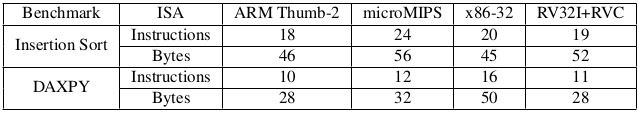
\includegraphics[width=0.8\linewidth]{ISA_Size_cmp.png}
		\bicaption{不同压缩指令集编译插入排序和双精度浮点乘加程序的代码大小比较。\citep{Patterson:2017:RRO:3202479}图 7.2.}{Instructions and code size for Insertion Sort and DAXPY for compressed ISAs. Figure 7.2 of \citep{Patterson:2017:RRO:3202479}.}
		\label{fig:sizecmp}
	\end{figure}
\end{enumerate}

ISA体系结构的演进发展已经有50多年的历史了,在诸如上述设计教训的沉淀下,最为基础核心的设计趋向于收敛。所以比MIPS晚诞生20多年的RISC-V能够站在后来者的角度审视之前诞生的众多指令集的优缺点,从设计开始就有一套清晰的规划,摒弃了很多包括上文提及的MIPS指令集设计中的缺陷,做到32位,64位,压缩变长指令集很好的统一,以简洁规整的形式呈现出来,最大化的简化了硬件指令译码的逻辑。同时,因为有了系统的规划,虽然目前特权态的有些规定还不是很明确,高性能的SIMD指令亦或是向量指令也不完善,但是对于处理器运行的模式规划确实非常明确有章法。另外,指令编码空间设计合理使得指令的可拓展性极强,以便日后之需。下面通过对比MIPS来具体分析RISC-V的特点以及简洁优美的设计考虑。

首先不同于几乎所有的先前的ISA,RISC-V是模块化的。核心是基础的ISA --- RV32I,简单而不失强大,足以运行整个软件栈。同时,RV32I是被冻结,也即永远不会改变,是稳定的,无论是对硬件设计人员或者软件设计人员都极为友好。其他的扩展功能的指令以可选的方式添加,比如也已经冻结的64位RV64I基础系列和M(乘除法)、A(原子指令)、F(单精度浮点)、D(双精度浮点)等拓展系列\citep{Patterson:2017:RRO:3202479}。
\begin{itemize}
	\item 用户态的对比:
	\begin{enumerate}[label=(\alph*)]
		\item RISC-V取缔了延迟槽的设计,使得ISA和处理器的微结构相对独立,同时编译出来的二进制代码量通常会比MIPS少。
		\item RISC-V取缔了HILO,但是32位的乘法和除法结果都是64位的,如何解决乘除法的结果存储问题。RISC-V选择软件来解决,对于每一个乘除法编译器都会得到两条连续的指令,一条得到低(商)32位,一条得到高(余数)32位,分别存储在不同的寄存器里。这样做的优势在顺序流水架构下不明显,但是在乱序的架构下就非常明显。本质上来讲,取缔HILO寄存器,把结果拆开存入通用寄存器中是一种统一编址的形式,乱序的重命名就只需要管理通用寄存器的映射关系即可,这样简化了重命名的结构。另一方面,就算有HILO寄存器,后续的指令要以乘除法的结果为源操作数时,也是要先通过mfhi,mflo指令读到通用寄存器中,多传导一次的导致效率不高的同时,还会占用指令空间。另外拆成两条连续指令来执行对于乱序的处理器只会增加少许额外的逻辑,这是因为reorder buffer会给每一条指令分配一个标识符id号,检测到连续的id号的指令就可以同时出结果,不用对乘除法算两次。
		\item RISC-V取缔了MIPS中的条件移动(conditional-move)指令,这是出于乱序设计简化的考虑。
		\item 不像MIPS用LWL,LWR来支持地址的非对齐访问。由于RISC-V指令可以是变长的,所以非对齐的访问是自然支持的。
		\item RISC-V没有算术指令溢出例外的规定,所以硬件不做处理。
		\begin{scala}
			add t0, t1, t2
			slti t3, t2, 0
			slt t4, t0, t1
			bne t3, t4, overflow
		\end{scala}
	
		将其完全移至软件处理,示例代码如上\citep{Patterson:2017:RRO:3202479}。
		\item RISC-V支持PC相对地址访问。在RISC-V中有这样一条指令AUIPC (add upper immediate to pc),该指令从指令中的20位立即数的基础上低12位填充0构成32位偏移量与当前的PC相加结果存到rd寄存器中。这样做的好处在于代码数据整体拷贝时依旧能够运行原有的程序,因为相对位置保持不变。下表\ref{tab:auipc}是用到AUIPC指令比较常用的情形\citep{user2017}:
		\begin{table}[!htbp]
			\bicaption{AUIPC指令常用的情形。}{The popular usage of AUIPC instruction.}
			\label{tab:auipc}
			\centering
			\footnotesize% fontsize
			\setlength{\tabcolsep}{4pt}% column separation
			\renewcommand{\arraystretch}{1.2}%row space 
			\begin{tabular}{lll}
				\hline
				Meaning & Base Instruction(s) & Pseudoinstruction \\%inserts table 
				%\cline{2-9}% partial hline from column i to column j
				\hline
				Load address & \begin{tabular}{@{}l@{}} \tt auipc rd, symbol[31:12] \\ \tt addi rd, rd, symbol[11:0] \end{tabular} & \tt la rd, symbol \\
				Load global & \begin{tabular}{@{}l@{}} \tt auipc rd, symbol[31:12] \\ \tt l\{b|h|w|d\} rd, symbol[11:0](rd) \end{tabular} & \tt l\{b|h|w|d\} rd, symbol \\ 
				Store global & \begin{tabular}{@{}l@{}} \tt auipc rd, symbol[31:12] \\ \tt s\{b|h|w|d\} rd, symbol[11:0](rd) \end{tabular} & \tt s\{b|h|w|d\} rd, symbol \\ 
				Floating-point load global & \begin{tabular}{@{}l@{}} \tt auipc rd, symbol[31:12] \\ \tt fl\{w|d\} rd, symbol[11:0](rd) \end{tabular} & \tt fl\{w|d\} rd, symbol \\ 
				Floating-point store global & \begin{tabular}{@{}l@{}} \tt auipc rd, symbol[31:12] \\ \tt fs\{w|d\} rd, symbol[11:0](rd) \end{tabular} & \tt fs\{w|d\} rd symbol \\ 
				Call far-away subroutine & \begin{tabular}{@{}l@{}} \tt auipc x6, offset[31:12] \\ \tt jalr x1, x6, offset[11:0] \end{tabular} & \tt call offset \\
				Tail call far-away subroutine & \begin{tabular}{@{}l@{}} \tt auipc x6, offset[31:12] \\
					\tt jalr x0, x6, offset[11:0] \end{tabular} & \tt tail offset \\
				\hline
			\end{tabular}
		\end{table}
		
	\end{enumerate}
	
	\item 特权态的对比:
	
	MIPS的特权态的管理用到的是Coprocessor 0(以下简称CP0),负责对虚实地址和例外处理进行管理。缺陷在于记录特权状态的寄存器的地址空间仅有区区5位32个,如果需要用到更多,则要引入CP1、CP2等等,导致整体地址空间的管理是独立而不连续的。为了避免这个不足,RISC-V的特权态寄存器有足足12位的地址空间,也即最多4096个寄存器可用。这4096个寄存器统称为Control and Status Registers (CSR),其地址空间的分配有清楚的规定,可以参见RISC-V特权态手册\textit{The RISC-V Instruction Set Manual Volume II: Privileged Architecture}\citep{privileged2017}。
	
	虽然RISC-V在运行操作系统等大型软件上的经验还不如MIPS雄厚,而且在手册上也明确说是草稿,一些规定不是很明确,比如处理器执行的初始地址自定义;虚拟地址的分配没有明确的规定(包括访问IO外设的地址、可以被缓存的地址)。但是其特权态的规范在这几年快速地发展,运行像Linux这样的操作系统已经绰绰有余。
	
	用模型的角度来分析,特权态本质上是用户态模型之上更高等级的状态集。这些状态同样是由寄存器来维护的。整个模型通过输入特权态指令来改变以及管理这些状态。那么怎么衡量一个ISA对于不同等级模式的刻画干不干净,就要看状态集以及这些状态的变化规不规整。
	
	如图\ref{fig:mode},RISC-V非常规整地将处理器的状态分为了3个等级:
	\begin{figure}[!htbp]
		\centering
		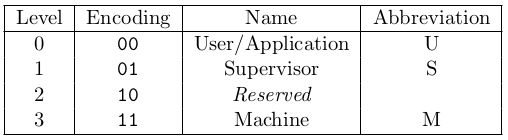
\includegraphics[width=0.5\linewidth]{Level.png}
		\bicaption{RISC-V的3个等级及其编码。\citep{privileged2017}表 1.1.}{RISC-V privilege levels and their encoding. Table 1.1 of \citep{privileged2017}.}
		\label{fig:mode}
	\end{figure}
	
	而这3个等级的2 bits编码均体现在特权指令的编码(用户态的指令不用这么编码是因为无论哪个等级都可以执行这些指令,而且省去这两位能够增加3倍的指令编码空间)和特权寄存器空间的编码。这样什么等级的指令执行在什么等级状态下处理器上,要修改什么等级的寄存器,非常的清晰明了。
	
	在三个等级中最为基础的就是Machine Level(以下简称M等级)。而M等级中基础的控制寄存器其实基本上和MIPS CP0寄存器是一一对应的。列举见表\ref{tab:sampleofCSR}:
	\begin{table}[!htbp]
		\bicaption{与MIPS CP0寄存器功能类似的CSR列表。}{The List of CSRs similar to MIPS CP0.}
		\label{tab:sampleofCSR}
		\centering
		\footnotesize% fontsize
		\setlength{\tabcolsep}{4pt}% column separation
		\renewcommand{\arraystretch}{1.2}%row space 
		\begin{tabular}{lll}
			\hline
			简称 & 全称 & 功能备注 \\%inserts table 
			%\cline{2-9}% partial hline from column i to column j
			\hline
			\tt mtvec    & \textit{Machine Trap Vector}       & 存储例外的跳转地址 \\
			\tt mepc     & \textit{Machine Exception PC}      & 存储例外发生的指令PC \\
			\tt mcause   & \textit{Machine Exception Cause}   & 指示例外发生的原因与类型 \\
			\tt mie      & \textit{Machine Interrupt Enable}  & 中断使能向量 \\
			\tt mip      & \textit{Machine Interrupt Pending} & 列举当前pending住的中断 \\
			\tt mtval    & \textit{Machine Trap Value} & 与MIPS中的BADADDR功能一致,存储例外访存地址 \\
			\tt mscratch & \textit{Machine Scratch}    & 一个指令长度的数据临时存储 \\
			\tt mstatus  & \textit{Machine Status}     & 与MIPS中的STATUS功能类似,存储处理器状态 \\
			\hline
		\end{tabular}
	\end{table}
	
	这里比较有特色的寄存器是mscratch。如果编写过或者看过MIPS上的操作系统内核,就会知道比如context switch和TLB的例外处理都需要用到K0和K1寄存器,这两个寄存器就是专门留给操作系统用于临时存储数据地址用的。虽然这样很高效,但是白白浪费了两个通用寄存器。另外一方面像context switch和TLB的例外处理是与M等级有关的,所以从设计的归类上来讲也应该归特权级别的寄存器管理而不是通用寄存器。这也是RISC-V更为干净的一种体现。
	
	在特权态中最为重要的一方面是内存管理,而一个最基本的考虑就是用户态不可信赖的程序要严格限制其只能访问到自己内存范围的内容。从RISC-V的手册\textit{The RISC-V Instruction Set Manual Volume II: Privileged Architecture}中,可以看得出其设计者在这方面下了很大的功夫。
	
	首先,RISC-V在M等级和User Level(以下简称U等级)之间设计了一种内存保护机制:Physical Memory Protection (PMP)。这样M等级就可以配置U等级程序能够访问的内存区域以及访问的权限。
	\begin{figure}[!htbp]
		\centering
		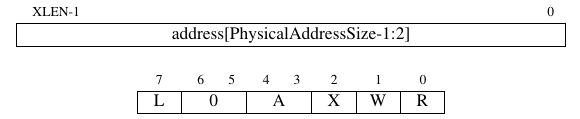
\includegraphics[width=0.7\linewidth]{PMP.png}
		\bicaption{PMP地址和配置寄存器。地址寄存器右移了2,如果物理地址比XLEN-1,那么高位填0. R, W和X域授权读,写,执行权限。A域设置PMP模式,L域锁住对应的PMP地址寄存器。\citep{Patterson:2017:RRO:3202479}图 10.7.}{A PMP address and configuration register. The address register is right-shifted by 2, and if physical addresses are less than XLEN-2 bits wide, the upper bits are zeros. The R, W, and X fields grant read, write, and execute permissions. The A field sets the PMP mode, and the L field locks the PMP and corresponding address registers. Figure 10.7 of \citep{Patterson:2017:RRO:3202479}.}
		\label{fig:pmp}
	\end{figure}
	上图\ref{fig:pmp}上半部分是PMP地址寄存器, 一般处理器会实现8-16个这样的寄存器;下半部分是PMP配置寄存器,为8-bit向量存储在pmpcfg的CSR寄存器里,负责授权或者禁止读、写、执行权限。当处理器在U-mode试图想要取指或者执行访存请求时,其地址将会被和PMP地址寄存器进行比较,如果地址大于等于$ i $号PMP而小于$ i+1 $号PMP。那么$ i+1 $号的PMP配置寄存器将会规定访问内存的模式,如果实际的访问方式逾越了配置寄存器里规定的权限,就会引发例外\citep{Patterson:2017:RRO:3202479}。
	
	对于嵌入式系统,PMP机制能够非常有效的对内存实行保护。但是其有两个缺点使之不适合更为复杂的系统和通用计算,分别是:
	\begin{itemize}
		\item 只支持最多16个内存区域,不能扩展性
		\item 这些区域都是连续的,有点像操作系统早期的\textbf{段}的概念。所以对内存的细粒度的片段化支持不好,而这也正是段的缺点
	\end{itemize}
	
	所以RISC-V的ISA必须支持基于页的虚拟内存机制。而这个特征直接主导了介于M等级和U等级中间的等级 --- supervisor mode(以下简称为S等级)的产生。
	
	但是引入S等级又会产生一个问题。RISC-V中所有的例外都是要将处理器的控制权转移到M等级的例外处理程序。但是大多数的Unix系统的系统调用包括例外是陷入系统内核,而系统内核又是运行在S等级的。如果先由系统将用户进程切换到内核,然后再由CPU硬件将内核S等级切换到M等级处理,最后M等级要重新路由到S等级,交给系统内核去退出系统调用\citep{Patterson:2017:RRO:3202479},这样效率就会大大降低。所以RISC-V提供了例外授权机制(exception delegation mechanism),这样中断和同步例外就能旁路到M等级,选择性的授权给S等级。而CSR寄存器 {\tt mideleg }(Machine Interrupt Delegation)和{\tt medeleg }(Machine Exception  Delegation) 正是这个机制的载体。对应于{\tt mip }和 {\tt mie }寄存器的exception code,举例来说,{\tt mideleg[5]} 对应于S等级的时钟中断,如果被置上,S等级的时钟中断将会把控制权转移到S等级的exception handler上而不是M等级的exception handler;同样,如果{\tt mideleg[15]}被置上,则会将store page faults授权给S等级来处理\citep{Patterson:2017:RRO:3202479}。不过需要注意的是,在某等级发生的例外永远不会转移控制权给更低的等级,具体来说就是在M等级发生的例外就只能M等级来处理;S等级发生的例外可能由M等级或者S等级来处理,取决于delegation的配置,但永远不会是U等级\cite{Patterson:2017:RRO:3202479}。
	
	RISC-V的分页方案命名方式为\textbf{SvX},比如32位的虚拟地址是\textbf{Sv32}, 其支持4GiB的虚拟地址,有两级页表,分别是$ 2^{10} $个 4MiB的页表,每个页表又有$ 2^{10} $个4KiB的基页。下图\ref{fig:SvX}是\textbf{Sv32}和\textbf{Sv39}的页表项(PTE):
	\begin{figure}[!htbp]
		\centering
		\begin{subfigure}[b]{0.7\textwidth}
			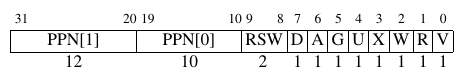
\includegraphics[width=\textwidth]{Sv32.png}
			\caption{}
		\end{subfigure}%
		
		\begin{subfigure}[b]{\textwidth}
			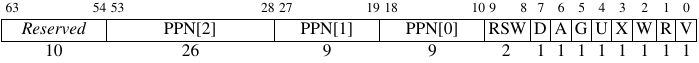
\includegraphics[width=\textwidth]{Sv39.png}
			\caption{}
		\end{subfigure}%
		\bicaption{RISC-V分页。\citep{Patterson:2017:RRO:3202479}图10.10和10.11. (a)RV32 Sv32页表项,(b)RV64 Sv39页表项。}
		{RISC-V SvX. Figure 10.10 and 10.11 of \citep{Patterson:2017:RRO:3202479}. (a)An RV32 Sv32 page-table entry(PTE), (b)An RV64 Sv39 page-table entry(PTE).}
		\label{fig:SvX}
	\end{figure}
	\textbf{Sv39}是$ 2^9\times 2^9\times 2^9 \times 2^{12} $的模式,是3级页表。如果物理地址比$ 2^{39} $还要大,RISC-V还提供了4级页表的\textbf{Sv48}方案。
	
	S等级用satp (Supervisor Address Translation and Protection)控制和状态寄存器管理分页系统,如下图\ref{fig:satp}:
	\begin{figure}[!htbp]
		\centering
		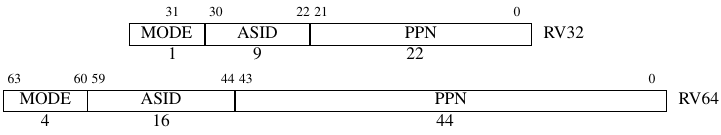
\includegraphics[width=0.7\linewidth]{satp.png}
		\bicaption{satp控制和状态寄存器 \citep{Patterson:2017:RRO:3202479}表 10.12.}{The satp CSR. Figure 10.12 of \citep{Patterson:2017:RRO:3202479}.}
		\label{fig:satp}
	\end{figure}
	在处理器进入S等级之前,M等级首先会写0到satp寄存器,禁止分页;然后等到进入S等级在初始化页表之后,处于S级内核就可以开始对satp寄存器进行操作来对内存进行分配了。
\end{itemize}

\subsection{Verilog和Chisel}

设计的实现是将抽象的逻辑层面想法概念用具体的语言严谨地描述出来,同样,设计处理器这样的硬件需要硬件的描述语言。当今主流的描述语言仍是90年代开发的Verilog。该语言设计参考的是C语言,最开始设计出来用作电路功能的仿真,因而有很多语法只适用于软件的仿真,不能作为物理电路的综合布局布线。可被综合的最常用的语句是组合逻辑的assign语句块和时序逻辑的同步always语句块。事实上这两种语句组合就能够满足绝大多数的电路设计的需求,其中就包括双发射乱序处理器。但是就像能够描述所有软件程序的汇编语言一样,Verilog的抽象等级太低,细节太多,描述电路的能力先天不足,主要体现在:
\begin{itemize}
	\item 语句的逻辑集成度不高,时常一个简单的逻辑代码量却不少。
	\item 变量名、函数名、参数名的管理机制原始落后,甚至都没有像C语言的struct结构体这种聚合化的设计。代码量大时,各个符号名称的关联往往复杂而混乱。
	\item 常用的简单逻辑代码复用度不高,代码复用基本上只能用Module这样一种单一的写法,容易冗余。
	\item 对多维的向量数组描述和聚合化操作支持不足。
	\item 没有成熟的类型系统,无论是Reg还是Wire都是对物理信号的刻画描述,粒度太小。
	\item 容易一不小心出现组合环,现有的编译器有很难跟踪。
	\item 要实例化不同参数的同一模块,只能一个个实例,做不到参数的数组化。
\end{itemize}

设想原本逻辑已经复杂不堪的双发射乱序处理器采用Verilog来描述,又会因为语言层面的弱势,使得实现起来异常的繁琐,复杂度得不到有效地控制。对这样的大工程的搭建、调试以及持续的优化、增量式演进都带来不小的挑战。

硬件工程师迫切需要一个更为高级的语言来解决上述Verilog种种缺陷,这就是Chisel。

Chisel没有那么神秘,并不是变革性的另一套硬件描述,而是包装在verilog之上具有面向对象和函数化编程特性的Scala脚本语言,是一种以Verilog中上述两种语句为基本块的更上一层的抽象。多一层的抽象就是为了解决Verilog表示能力不足的缺陷。比如Chisel支持面向对象里的类和对象、接口以及多态与继承的特性,可以很好地复用代码,有条理地管理变量名、方法名和参数名;另外函数式的编程可以用来很便捷的描述简单的电路逻辑,增强对多维数组操作的支持。对应的,Chisel的编译器主要工作就是将抽象的Scala代码转化为低级的Verilog,而且是完全可以被综合和物理实现的Verilog (所以是否是可综合的电路根本不需要顾虑)。类似于JAVA编译器将JAVA编译成汇编代码。

Chisel和JAVA都是强类型的语言(Chisel的类型继承关系如图\ref{fig:type} (\url{https://chisel.eecs.berkeley.edu/2.2.0/manual.html}),在编译的时候会做类型检查,从而避免很多因为类型不当导致的逻辑错误。而Verilog和汇编都是没有类型的概念的,一个32位的逻辑寄存器,汇编可以任意的操作而不用在乎这个寄存器代表的是整型还是字符型,同样,Verilog对一个32bit的Wire和Reg向量也可以任意操作。正是因为这种毫无约束的操作,使得用汇编或者Verilog编程都会比Chisel或者JAVA来得繁琐而易出错。但是略显不同的是,一个初学者可以在不知道汇编语言的情况下就能够掌握JAVA语言这样的抽象等级高的语言,但是却不能在没有熟练运用Verilog中的两个基本语句的前提下掌握Chisel。换言之JAVA对于汇编的抽象是彻底的,而Chisel对于Verilog的抽象是不彻底的,所以Chisel适用于有一定硬件设计工程经验的人,而不适用于上手设计电路的初学者。
\begin{figure}[!htbp]
	\centering
	\begin{subfigure}[b]{0.35\textwidth}
		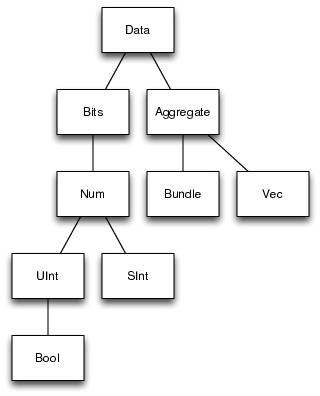
\includegraphics[width=\textwidth]{type-hierarchy.png}
		\caption{}
		\label{fig:type}
	\end{subfigure}%
	~%add desired spacing
	\begin{subfigure}[b]{0.65\textwidth}
		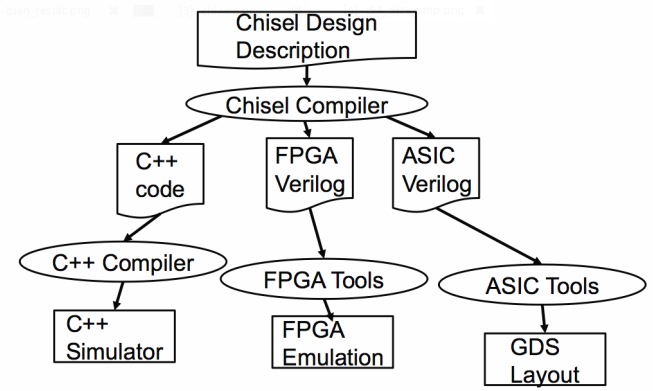
\includegraphics[width=\textwidth]{Chisel_data_flow.png}
		\caption{}
		\label{fig:design_flow}
	\end{subfigure}
	\bicaption{Chisel的类型层次结构和设计流。(a) Chisel类型系统,(b) 基于Chisel的设计流程框图。\citep{lab1}图 1.}{Chisel type hierarchy and Chisel Design Flow. (a) Chisel type hierarchy, (b) Chisel Design Flow. Figure 1 of \citep{lab1}.}
	\label{fig:chisel_into}
\end{figure}

从Chisel设计流程框图\ref{fig:design_flow}可以发现,首先Chisel通过编译器不仅能够编译成Verilog,还能编译成C++代码再通过C++的编译器得到C++的模拟器。工程实践证明,C++模拟器仿速度非常快,跑500遍dhrystone仅仅需要1秒。其次Chisel编译器可以针对不同的硬件平台编译采用不同的优化。甚至得到的电路时序比人写的Verilog对应的电路还要好。

但是电路描述高级语言化首先需要克服电路方面特有的两大障碍:
\begin{enumerate}
	\item 时序逻辑高级语言应该如何描述?
	\item 随着语言的高级化,会不会使得电路的编写模糊化,使得所写的电路很难对应到实际的物理电路上,就像高级语言对垃圾回收做了透明化一样。这恰恰是硬件的工程师所不愿意看到的,因为电路设计要了解电路的所有实现细节。
\end{enumerate}

那么Chisel是如何成果性地打消上述的两个障碍和顾虑的呢?那就要看Chisel是如何进行抽象的。
\begin{enumerate}[label=(\alph*)]
	\item 组合电路的对应于Verilog中的Wire,赋值用assign语句,也可以直接在Wire型变量定义的时候赋值。而Chisel首先用的就是两类最基本的数据类型来描述,分别是UInt和Bool。Bool只是为了强调变量是1 bit的代表真假布尔逻辑的变量。而Wire型变量的赋值有两种形式:
	\begin{itemize}
		\item 初始定义的 \textbf{=} 运算符 
		\begin{scala} 
			val pc = Wire(UInt())
		\end{scala}
		
		如上并不是真正的赋值,而是类型的申明。UInt的括号中可以传入位宽的参数,如果省略,Chisel会在编译的时候自动在以后的真正赋值中推导出来,所以还是非常人性化的。
		\item 因为val在Scala中是不可变量,也就是变量名指针所指的对象不能更改,所以chisel中引入\textbf{:=}运算符来进行再赋值。
		\begin{scala} 
			pc := pcReg + 4.U 
		\end{scala}		
	\end{itemize}
	\item 时序电路对应于Verilog中的reg,赋值需要用到always语句。而在Chisel对其进行了抽象,首先它没有具体的类型,是一个Reg的元器件。其次这个元器件有两端 --- input和output。而output可以理解为input信号延迟一周期的副本。严格来讲,Reg型变量的类型可以定义为input端所连的变量的类型,在reg类型变量的定义中还可以指明reset的初始值。如下例:
	\begin{scala}
		val pcReg = Reg(next = pcNext, init = 0.U(32.W))
	\end{scala}
	在当前的版本的Chisel中,时钟和复位是全局信号,是隐式申明的\citep{chisel2017}。
	这样Reg型的变量的更新可以做到简单一行的赋值代码,和组合逻辑Wire型变量一样使用\textbf{:=}运算符。
	\item 由于赋值运算符的统一,Chisel对于wire类型和reg类型的变量统一抽象为了电路上的节点(node)。整个电路图就是由node组成的图。具体来讲,如果是纯组合逻辑,那么这个图就是有向无环图,所以Chisel是可以对于设计中出现的组合环会进行非常精确的报错,指出相同的开始节点和结束节点,从而规避了仿真中出现的奇怪的现象。唯一存在有环的情况是时序电路。而且依据这个图,可以用verilator工具生成高速的C++的simulator\citep{chisel2017}。
	\item 变量统一抽象为电路节点反过来将\textbf{:=}运算符的意义统一了 --- 将右手表达式代表的节点组合逻辑连线到左手变量代表的目的节点上。但是略有差异而且需要注意的是,如果涉及到Reg型变量\textit{x},因其具有两端,若\textit{x}出现在右手表达式,用的是output端;若\textit{x}出现在左手表达式,用的是input端\citep{chisel2017}。
	
	\item 有了基础的抽象,Chisel可以在其上利用面向对象的方法和继承的手法自定义构建更为大型,更为抽象的数据结构。
	\item 类比在Verilog对于模块的刻画用了module的写法,Chisel采用用户自定义类去继承称为Module的父类的写法,并且对于模块的接口,还定义了一个IO的类。如下例\citep{chisel2017}:
	\begin{scala}
		class Mux2 extends Module {
			val io = IO(new Bundle{
				val sel = Input(UInt(1.W))
				val in0 = Input(UInt(1.W))
				val in1 = Input(UInt(1.W))
				val out = Output(UInt(1.W))
			})
			io.out := (io.sel & io.in1) | (~io.sel & io.in0)
		}
	\end{scala}
	这里的Bundle是一个Chisel里的基类,类似于C里面的\textit{Struct}。但是如上述例子所展示的,可以不需要对这个结构体预先定义而直接新建一个匿名的结构体,然后作为参数传入IO的构造方法中,最后将其赋值给IO。这种写法相比于Verilog里最大的好处在于在Module的内部的逻辑中,Chisel的代码更加清晰。端口因为都带有\textit{io.}的前缀,引用或者赋值一目了然。这样增加了代码的可读性。
\end{enumerate}

经过上面的分析,Chisel语言依旧能够呈现统一时钟复位电路的所有细节。如果尚有缺点,也是因为目前屏蔽了clock和reset,默认为统一时钟同步复位,还不支持异步电路。这个在Chisel的文档里也给出了解释:纵然有交叉时钟的设计需求,但是现代设计方法中也是在每一个同步的电路岛屿中开发与验证的\citep{chisel2017}。

下面用三个例子来展示Chisel在电路设计的简便之处:
\begin{enumerate}
	\item 下面代码\citep{chisel2017}灵活运用了面向对象和可配置参数化函数(类似于C++的template)的语言特性。首先是通过面向对象的继承来充分复用已有的代码逻辑,其次不同功能的Filter利用$\lambda$-函数作为参数传入,来充分复用不同Filter相同逻辑的部分,与此同时并没有掩盖电路的细节。
	\begin{scala}
		abstract class Filter[T <: Data](dtype: T) extends Module {
			val io = IO(new Bundle {
				val in = Input(Valid(dtype))
				val out = Output(Valid(dtype))
			})
		}
		class PredicateFilter[T <: Data](dtype: T, f: T => Bool) extends Filter(dtype) {
			io.out.valid := io.in.valid && f(io.in.bits)
			io.out.bits  := io.in.bits
		}
		object SingleFilter {
			def apply[T <: UInt](dtype: T) = 
			Module(new PredicateFilter(dtype, (x: T) => x <= 9.U))
		}
		object EvenFilter {
			def apply[T <: UInt](dtype: T) = 
			Module(new PredicateFilter(dtype, (x: T) => x(0).toBool))
		}
		class SingleEvenFilter[T <: UInt](dtype: T) extends Filter(dtype) {
			val single = SingleFilter(dtype)
			val even   = EvenFilter(dtype)
			single.io.in  := io.in
			even.io.in    := single.io.out
			io.out        := even.io.out
		}
	\end{scala}
	
	\item 拷贝于毕业设计代码中的顶层文件。可以看到其中颇具特点的运算符\textbf{<>}(在Chisel的术语里叫做\textit{Bulk Connections}),大大简化了模块实例化后互相连线的逻辑,相当于一些输入输出信号集合整体的连线。
	\begin{scala}
		class Core(implicit conf: CPUConfig) extends Module with BTBParams {
			val io = IO(new Bundle {
				val imem = new AxiIO(conf.xprlen)
				val dmem = new MemPortIo(conf.xprlen)
			})
			val frontEnd = Module(new FrontEnd)
			val backEnd  = Module(new BackEnd)
			frontEnd.io.mem  <> io.imem
			backEnd.io.mem   <> io.dmem
			frontEnd.io.back <> backEnd.io.front}
	\end{scala}
	
	\item 拷贝于毕业设计代码中的写回结果总线监听逻辑。发射队列有nEntry项,每一项存有一条待发射的指令,需要监听两个源操作数,写回总线结果对应于代码中的\textit{io.bypass}。下面短短几行的代码里就涵盖了将写回总线的寄存器地址和有效使能信号逐一与发射队列里的每一项待发射指令的每一个源操作数进行比对,判断是否成功监听的逻辑。Chisel对于数组聚合化操作的强大描述能力可见一斑。
	\begin{scala}
		for (i <- 0 until nEntry) {
			for (j <- 0 until 2) {
				inst_ctrl.snoop(i)(j) := issue.snoop(i)(j).valid ||
				io.bypass.map(b => 
				b.addr === issue.snoop(i)(j).addr && b.valid).reduce(_||_)
			}
		\end{scala}
		
	\end{enumerate}
	
	\subsection{RISC-V开源仓库}
	RISC-V近年的流行和其开源仓库是相辅相成的,目前在开源的工程下至较为成熟的处理器设计实现以及整套SoC的环境,上至各种软件栈一应俱全。使得大至一个国家如印度,中至一些企业组织如lowRISC,小至一个个独立的研究个体都愿意加入到RISV-C的开发中来。
	
	具体对设计影响较大的几个开源工程有开发语言Chisel,双发射乱序处理器BOOM及其设计文档和RISC-V整套在x86 host机上处理器设计的调试环境。
	
	\section{研究范围}
	
	一个人做出一个功能齐全,能够运行操作系统和整套软件栈的双发射乱序处理器,在半年时间内几乎是不可能完成的。所以研究的范围应该集中在乱序的调度,分支的预测以及取指部件的高效取指上,最后能够运行简单嵌入式程序来初步验证处理器正确性和评测性能即可。
	
	在摘要中已经提及了必要的简化方案,更具体的方案包括:不支持MMU以及分页机制;取指为了实现取指宽度大于1实现了icache并且对外是AXI接口,测试的时候带有随机的取指延迟;访存虽然支持访存延迟,但没有实现dcache,对外也不是AXI接口,访存过程几乎是一个周期的同步时序。
	
\chapter{材料与方法}\label{chap:Material_approach}
%With speculative execution, it calculates memory addresses and initiates cache refills early
\section{相关工作与材料}\label{sec:meterial}
	前有经典的Alpha 21264和MIPS R10000成熟产品,后有开源的RISC-V BOOM处理器设计,都是非常优秀的相关工作。而它们的设计报告文献作为宝贵的材料同样值得参考与借鉴。吸收它们的优秀结构设计并灵活运用到自己的处理器设计当中。
	\subsection{Alpha 21264}\label{subsec:alpha}
	
	Alpha 21264是处理器设计历史上高性能的代表之作。下面从\textit{THE ALPHA 21264 MICROPROCESSOR}\citep{Alpha21264}这篇技术报告分析Alpha 21264的微结构设计。
	
	首先Alpha 21264整体的流水级模块级框图\ref{fig:alpha_stage}一共切分成了7个大的阶段。
	\begin{figure}[!htbp]
		\centering
		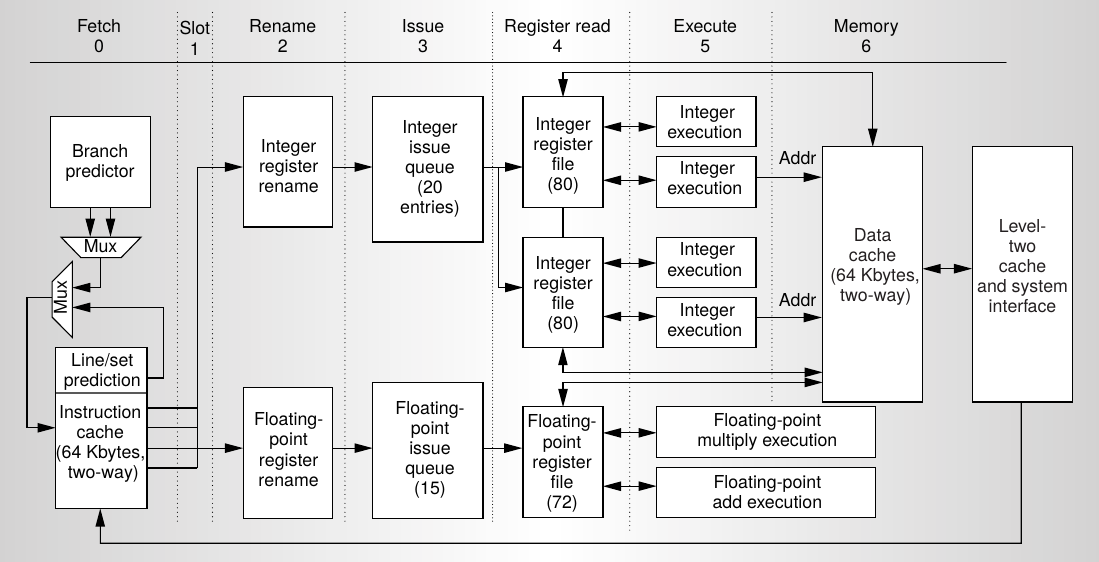
\includegraphics[width=0.8\linewidth]{21264}
		\bicaption{Alpha 21264流水线阶段。\citep{Alpha21264}图 2.}{Stages of the Alpha 21264 instruction pipeline. Figure 2 of \citep{Alpha21264}.}
		\label{fig:alpha_stage}
	\end{figure}
	
	从第0级的取指开始往流水线的下游方向逐级分析一些设计的亮点。
	\begin{enumerate}[label=(\alph*)]
		\item \textbf{取指}。21264为了提高取指的效率,着重强调了两个设计,一是icache的行和路预测,二是分支跳转预测。
		
		由于21264的icache采用的是两路组相连,一种方案是把行对应的两个路都读出来,然后在做二选一逻辑,不过这样电路延迟就增加了,而且可拓展性也不好,到四路的延迟更大。所以21264选择了另外一种方案 --- 路预测,采用和分支预测相似的两位饱和计数的技术,对于大多数程序而言正确率都能达到85\%$ \sim $100\%,猜得准的同时猜错代价很小,绝大多数情况下只有1个周期\citep{Alpha21264}损失。所以采用路预测对电路主频的提高收益大于损失的周期数。
		
		与icache路预测情况不同,21264最多容纳80条指令乱序执行,转移指令猜错代价很大。所以分支预测就成为了提高21264效率非常重要的一环。为了追求预测的正确率,21264实现了复杂的锦标赛预测方案,动态的选择两种类型的分支预测器的预测结果 --- 一是用跳转指令本身的跳转历史,二是用全局的跳转历史。预测准确率比采用更大的表独立各采用上述两种方案更好,达到90\%$ \sim $100\%\citep{Alpha21264}。具体来看,21264一共维护了3个表,结构如图\ref{fig:branch_21264}所示。
		\begin{itemize}
			\item 一张局部历史表,能够存放1024条指令10 bits的自身跳转历史,面积$ 1024\times 10 $ bits.
			\item 一张全局预测表,配以一个12 bits的全局历史,所以有4096项,每一项是2位饱和计数器,面积$ 4096\times 2 $ bits.
			\item 一张选择表,用来选择两种预测机制中更好的一个,和全局预测表一致,共有4096项,也采用两位饱和计数器,面积$ 4096\times 2 $ bits.
		\end{itemize}
		\begin{figure}[!htbp]
			\centering
			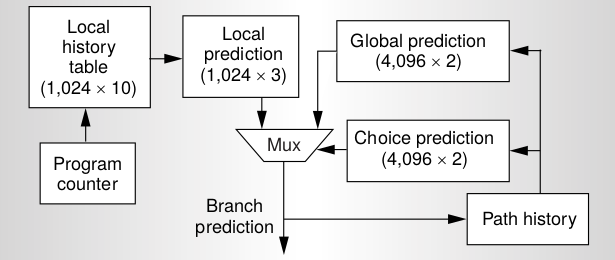
\includegraphics[width=0.7\linewidth]{branch}
			\bicaption{21264锦标赛分支预测框图。\citep{Alpha21264}图 4.}{Block diagram of the 21264 tournament branch predictor. Figure 4 of \citep{Alpha21264}.}
			\label{fig:branch_21264}
		\end{figure}
		\item \textbf{重命名与乱序发射}。在21264的设计中,乱序的部分为了效率考虑,采用主频更高的时钟域。
		
		一个周期最多能够取回4条指令,先锁存一个周期,然后在CAM形式的重命名表中进行重命名和寄存器的分配。需要注意的是,和MIPS一样,Alpha在重命名阶段要特殊处理条件移动指令的映射关系。重命名完毕消除了写后写和读后写的冲突,但是依旧保留了写后读冲突。之后将指令写入发射队列中。发射队列采用分离式,分为整数指令队列和浮点指令队列,最多可以动态发射出6条指令,四条整数指令,两条浮点指令。使用记分牌来判断指令的操作数是否准备就绪。发射的细节上,微结构上有一个20项的定点队列和一个15项的浮点队列,队列只发射的是那些操作数都已经准备好的指令。与此同时,队列由仲裁器来决定填入新的指令。上述模块的逻辑可以由图\ref{fig:rename_21264}来直观的描述。
		\begin{figure}[!htbp]
			\centering
			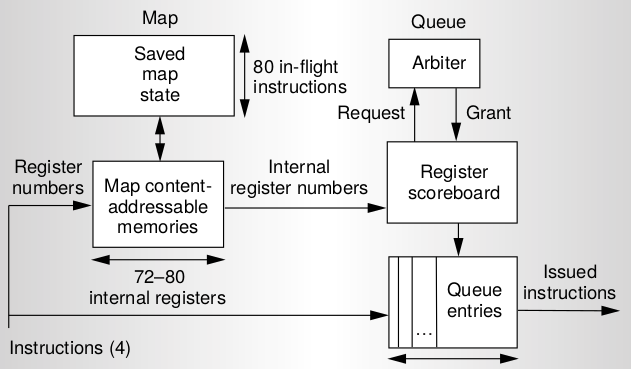
\includegraphics[width=0.6\linewidth]{rename}
			\bicaption{21264寄存器重命名以及出入队列阶段框图\citep{Alpha21264}图 5.}{Block diagram of the 21264’s map (register rename) and queue
				stages. The map stage renames programmer-visible register numbers to
				internal register numbers. The queue stage stores instructions until they
				are ready to issue. These structures are duplicated for integer and floating-
				point execution. Figure 4 of \citep{Alpha21264}.}
			\label{fig:rename_21264}
		\end{figure}
		上图中有一个Saved map state模块,非常重要,它的作用是转移预测错误的恢复处理器状态。注意该表有80项,也即每一条指令分配一项,这样处理器可以从任何一条指令之后精确地恢复状态,而不会受到跳转指令数量的约束。但是缺点是非常消耗资源。当然不光是转移预测错误的恢复,例外中断的状态恢复同样也是用这个表的,但和分支预测错误的恢复机制略有不同。
		\item \textbf{乱序执行引擎}。由于发射队列每一周期能够发射6条指令,所以引擎一共有6条执行流水线。
		
		21264具有特色地将整数寄存器堆分裂为两个集群,均有重复的80项。对应的属于整数的4条流水线被均等的分配到了两个集群下。虽然这样增加了集群之间互相广播的电路延迟和周期数,但是却使得设计更加简单快速。最根本的原因是减少寄存器堆的读端口数目。如果不分为两个集群,每条指令需要两个操作数一共就需要8个读端口,加上寄存器堆有80项,物理布局布线之后的时序非常的差,远远不如只有4个读端口的情况。Alpha这个用空间换时间的做法也是无奈之举。这也给后来的设计者一种警示,为了处理器的主频,必须要控制寄存器堆的读端口数量。
		\item \textbf{指令的提交与退出}。指令是按照次序提交退出的。
		
		在21264设计文档中给出最为有用的信息是每一条指令都要带着之前旧的目的物理寄存器号,并在顺序提交退出后回收这个该物理寄存器。首先这个机制能够维护有远远不断的物理寄存器可以再生分配,其次说明了这个机制有正确性的保障。所以毕业设计中的做法和Alpha的做法保持一致。

		\item \textbf{内部访存部件设计}。
		
		为了降低访存的平均延迟,Alpha 21264在访存上做了很多不惜成本的设计,将性能做得非常强悍。主要体现在:一个周期能够执行两条乱序的访存请求,也即首先dcache即必须是双端口的;访存系统能够同时追踪32条in-flight的store指令,32条in-flight的load指令和8条in-flight的指令或者数据cache miss;dcache是64KB,2路组相连的结构\citep{Alpha21264}。处理器内部访存控制结构采用经典的load queue(LDQ)和store queue(STQ)数据结构。每个队列均有32项和上述可以同时追踪的load/store指令数量一致\citep{Alpha21264}。毕业设计中基本的设计参考的就是21264的设计,但是做了一些面积功耗的优化与改进。
		\item \textbf{内部memory系统}。21264设计了高带宽和低延迟的memory系统。
		
		这篇设计文档最后花了较多的篇幅来介绍,包括cache预取,填入和替换策略以及总线的介绍,以及用8项的miss address file (MAF)来同时追踪上文提到的8条in-flght cache miss访存请求的机制。内部memory系统是非常复杂的一个领域,在毕业设计中出于简化的考虑不会继续做深入的分析和设计。
	\end{enumerate}
	
	\subsection{MIPS R10000}\label{subsec:r10000}
	
	R10000是一款四发射乱序处理器,执行引擎有五个流水线;为了隐藏访存延迟,R10000用了两级均为两路组相连写回的cache,并且是非阻塞式的,也即一个cache行的miss不会阻塞另外cache行的访问;在处理器内部in-flight的指令数最多有32条\citep{MIPS1996}。处理器的整体设计参见模块框图\ref{fig:r10000_block},流水线(图\ref{fig:r10000_pipeline})级数的编号是从1开始的。
	\begin{enumerate}
		\item 第一级发出取指请求,并对齐下一周期的四条指令。
		\item 第二级对取回的指令做译码然后进行重命名,同时计算跳转分支指令的目的地址反馈到取指单元.
		\item 第三级将重命名完的指令写入发射队列中,直到操作数都已经准备好,才能从队列中发射出来。在后半个周期的时候读寄存器堆获取源操作数。
		\item 第四级开始执行,整数指令需要一个周期,load指令需要两个周期,浮点指令需要三个周期,
		\item 写回是在得到结果后一个周期的前半个周期。
	\end{enumerate}
	\begin{figure}[!htbp]
	\centering
	\begin{subfigure}[b]{0.7\textwidth}
		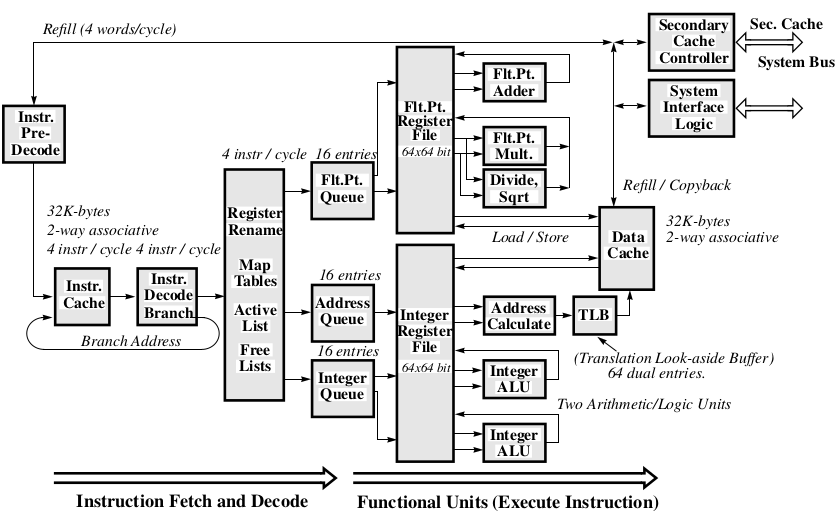
\includegraphics[width=\textwidth]{r10000_block}
		\caption{}
		\label{fig:r10000_block}
	\end{subfigure}
	\begin{subfigure}[b]{0.7\textwidth}
		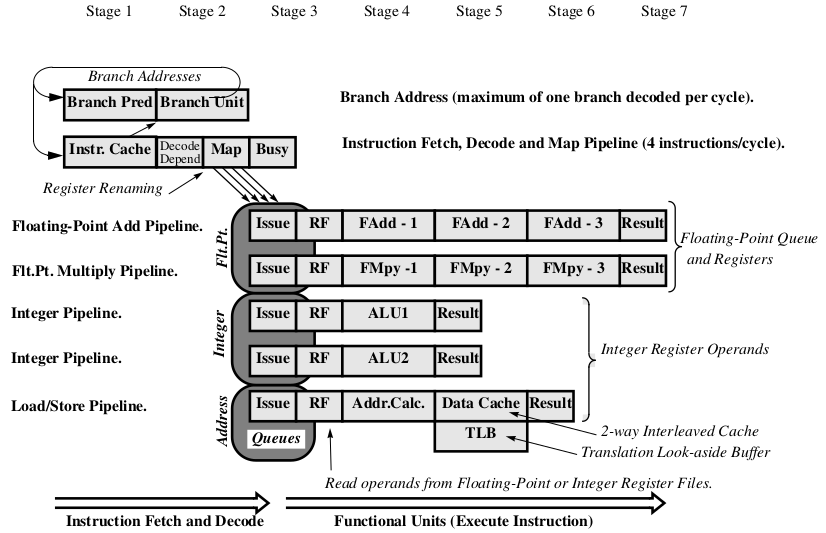
\includegraphics[width=\textwidth]{r10000_pipeline}
		\caption{}
		\label{fig:r10000_pipeline}
	\end{subfigure}
	\bicaption{MIPS R10000整体设计。\citep{MIPS1995}图2和3. (a) R10000模块框图,(b) R1000流水线。}{MIPS R10000 overall design. Figure 2 and 3 of \citep{MIPS1995} (a) R10000 Block Diagram, (b) R10000 Pipelines.}
	\label{fig:r10000_total}
	\end{figure}

	与Alpha 21264相似之处在于对整数指令和浮点指令采用了分离式的处理方案。但是与Alpha 21264相比,性能却差了很多。这与微结构的设计是分不开的。仅仅是通过观察两者的整体设计图以及一些最基本的参数,不考虑转移预测率和访存的性能,都不难找到R10000与21264之间差距的几点原因:
	\begin{enumerate}[label=(\alph*)]
		\item 因为都是采用分离式结构,只需对比整数指令。R10000最多支持32条in-flight的指令乱序调度,但是21264却支持80条,是R10000的两倍多,所以对指令的并行性有更大程度的挖掘。还有一点是,由于两者超标量宽度同样是4,但是由于R10000允许的in-flight指令比21264少太多,很容易导致发射队列塞满而阻塞取指部件供应指令。
		\item 流水级的切分不合理,导致时序太差。如果用统一的从1开始编号,那么意味着21264是在第5个周期读寄存器堆的,而R10000在第3个周期就要读取了。足足提前了两个周期,换言之,R10000将21264五个周期的工作压缩到3个周期,电路时序之差就可想而知了。有两点特别突出:第一,从icache同步读回的指令,组合逻辑就要做译码,重命名,算跳转地址,所以第二级的电路延迟非常大;第二,第三级中要先从16项的队列中选出发射的最多可以有两项(定点队列),然后组合逻辑去读寄存器堆,这一级的时序也是非常紧张。
		这两点Alpha 21264都分别用两个周期来做的,所以R10000少的两周期就是这么来的。
		\item 在21264中已经面对的问题 --- 对于寄存器堆的读端口要控制。为此21264还专门做了两份重复的寄存器堆来缩减读端口。如果看配置,21264是80项,有4个读端口;而MIPS则是64项,有6个读端口。因为读端口多了两个,所以单就寄存器堆的时序上,R10000就不如21264,更何况21264是用一整级来做读寄存器堆的逻辑的。
	\end{enumerate}
	
	综上所述,在21264主频已经达到500$ \sim $600MHz的时候,R10000主频只能做到200MHz;所以在SPEC95性能测试程序上,21264定点程序在30分以上,浮点程序在58分以上,而R10000定点程序峰值为9分,浮点程序的峰值为19分,是21264性能的1/3不到\citep{Alpha21264,MIPS1996}。 但这些并不影响R10000同样存在一些值得借鉴的设计思路,下面梳理一下R10000的一些设计亮点:
	\begin{enumerate}[label=(\alph*)]
		\item 取指部件。
		
		\citep{MIPS1996}提出的设计思路是处理器取回来的指令带宽上要高于执行部件,将队列填充满非常重要,这样基本上就能在每一个周期都找到可以被发射的指令。和一般取指需要取指宽度对齐不同,R10000虽然取指宽度是4字(1指令/字),但是可以在16字指令cache行中以任意字对齐,这样可以提高取值的效率。通过一个对cache读出放大器简单的修改,基本上是四选一的逻辑。同时,为了简化连续的取指的时序,当发射队列或者活跃表已经满时,指令会被先进入一个八字的指令缓存\citep{MIPS1996},也即最多可以缓存8条未被译码的指令。这一点已经借鉴到了自己的处理器设计当中,参见第3章节。
		\item 分支跳转单元。
		
		R10000在这一方面做的也没有21264性能高,体现在两个方面。第一,预测策略上,只有一个简单的有512项的两位饱和计数器,在Spec92整点程序中预测率也只有87\%\citep{MIPS1996}; 第二,设有分支栈,每当有译码到分支指令时,就会把处理器的状态压入栈中,作用是当分支预测错误处理器能够恢复到错误跳转前的状态。对比21264为每一个指令都存储对应的状态的做法,R10000显然会受限于高分支指令占比的程序以及程序片段。为了快速恢复,撤销掉分支预测错误后面的指令,R10000的每一条指令都带有4-bit的掩码,对应于分支栈,指示依赖于哪一项分支跳转。如果依赖该条分支指令,该位掩码置上。当分支预测错误就可以根据掩码的信息来撤销误取的指令。
		\item 寄存器重命名。
		
		见图\ref{fig:r10000_rename},不同于21264的CAM重命名表,R10000的重命名表是RAM的形式。考虑到HILO寄存器的存在,并且排除永远为$ 0 $的r0的寄存器,整数指令的重命名表是一张$ 33\times 6 $-bit的16读端口4写端口的RAM\citep{MIPS1996}。在重命名的相关控制逻辑上,R10000使用了三个数据结构 --- Free list, Active list和Busy-bit tables. 简言之,这三个数据结构的作用分别是:Free list负责记录更新未被使用的寄存器号用来进行物理寄存器的分配;Active list作用相当于Reorder buffer,记录在处理其中in-flight的活跃指令;Busy-bit tables用来指示当前物理寄存器中的值是否有效。
		\begin{figure}[!htbp]
			\centering
			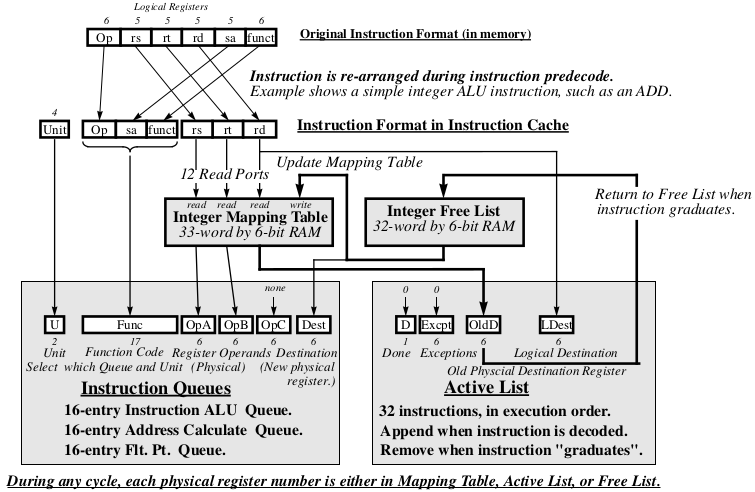
\includegraphics[width=0.7\linewidth]{r10000_rename}
			\bicaption{R10000寄存器重命名机制图解。\citep{MIPS1995}图4.}{Register Renaming of MIPS R10000. Figure 4 of \citep{MIPS1995}.}
			\label{fig:r10000_rename}
		\end{figure}
		
		\item 发射队列。
		
		除了常规的定点队列和浮点队列外,R10000还增加了一个地址队列,也可以被称为访存指令队列。为循环队列的形式,有16项。但这也不是新奇的设计,功能上和21264中的LDQ和STQ设计类似,只是将load和store指令统一存放在一起而已。
		\item 其他方面如运算单元的设计和内存层级结构并不在毕业设计范围之内,所以不做探讨。
	\end{enumerate}

	\subsection{RISC-V BOOM}\label{subsec:BOOM}
	
	BOOM是伯克利分校为了向学术界和工业界推广RISC-V ISA而设计出来的乱序处理器,其全称为The Berkeley Out-of-Order Machine。首先BOOM是伯克利分校在校的博士生们设计的,主要参考的是之前提到的两款经典的处理器Alpha 21264和MIPS R10000. 采用Chisel语言来编写,而且由于不是采用和21264、R10000类似的定制电路,诸如队列的项数,cache的大小,甚至发射指令数量都是参数化可配置的,所以强调参数的具体数字是没有多大意义的。但是像超标量宽度为2的参数基本上是固定的,也即BOOM的取指单元每一拍取回两条指令。
	
	BOOM经历了先后两代的演化,从版本1(BOOMv1)到版本2(BOOMv2)的变化能够十分真切的看出其在微结构上的瓶颈、改进重点和设计权衡。
	
	BOOMv1在流水级的切分参考了R10000,分成了六级 --- 取指、译码/重命名、发射/读寄存器、执行、访存、写回\citep{Celio:EECS-2017-157}。这种流水线的切分方案在MIPS R10000章节\ref{subsec:r10000}已经分析过是极不合理的,电路主频做不好。而且BOOMv1的整数寄存器和浮点寄存器是统一的,这样导致的后果是寄存器的项数和读端口数量(共有7个读端口和3个写端口)都很多;另外,BOOMv1采用了统一的发射队列,发射指令数量为3,也即在同一个队列里要一个周期要选出3条准备就绪的指令发射\citep{Celio:EECS-2017-157}。这样的设置同样极不合理,综合得到的电路变得异常复杂,时序会异常不好。综上,虽然IPC的比较上BOOMv1比BOOMv好了20\%\citep{Celio:EECS-2017-157},但是BOOMv1微结构设计糟糕,参考意义不大。下面着重来分析BOOMv2的值得借鉴的微结构设计:
	\begin{figure}[!htbp]
	\centering
		\begin{subfigure}[b]{.45\textwidth}
			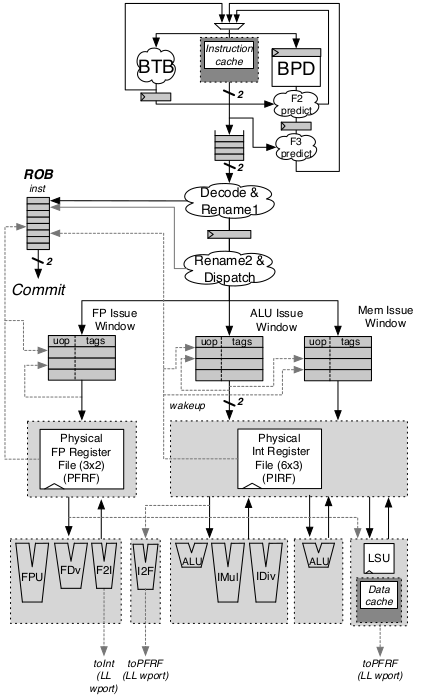
\includegraphics[width=\textwidth,height=12cm]{boomv2_tot}
			\caption{}
			\label{fig:boom_total}
		\end{subfigure}\qquad
		\begin{subfigure}[b]{.45\textwidth}
			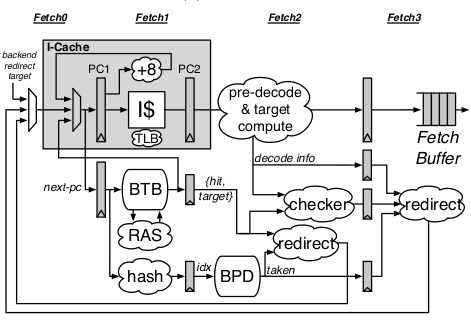
\includegraphics[width=\textwidth,height=5.5cm]{boom_ftend}
			\caption{}
			\label{fig:boom_ftend}
			
			\vspace{2ex}
			
			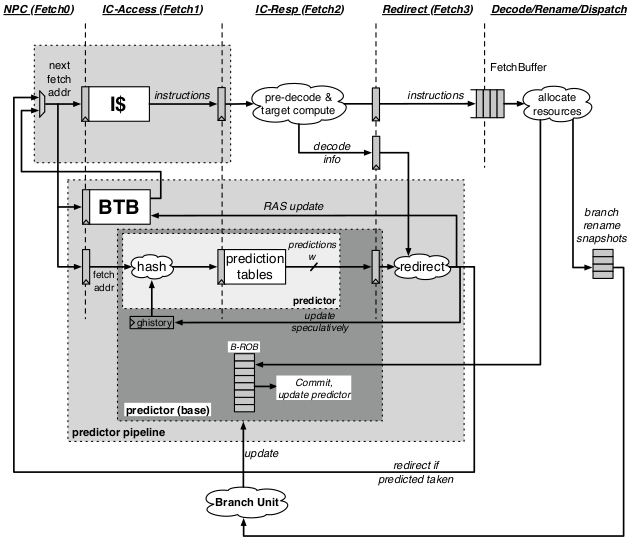
\includegraphics[width=\textwidth,height=5.5cm]{branch_fig_4_3}
			\caption{}
			\label{fig:boom_predictor}
		\end{subfigure}
		\bicaption{BOOMv2的全局设计以及前端设计图。\citep{Celio:EECS-2017-157}图2(b)和3(b), \cite{Celio:EECS-2018-151}图4.3. (a)BOOMv2的全局设计。(b)前端设计图。 (c)前端细节设计图。}{BOOMv2 overview and Frontend design. Figure 2(b) and 3(b) of \citep{Celio:EECS-2017-157}, Figure 4.3 of \cite{Celio:EECS-2018-151}. (a)BOOMv2 overview, (b)Frontend design, (c)Frontend design with more details.}
		\label{fig:boomv2}
	\end{figure}

	\begin{enumerate}[label=(\alph*)]
		\item 前端的设计。
		
		在BOOM相关的论文\citep{Celio:EECS-2017-157,Celio:EECS-2018-151}中,强调了前后端的概念。事实上,这是一个非常优秀的理念,很值得借鉴到自主的处理器设计之中。前端负责项后端供应指令,连续不断的指令流的供应就显得尤为重要。为了预测率并且权衡面积、关键路径延迟和预测错误流水线的取消开销等多方面的考虑,在BOOMv2的前端中,加入了多种不同的转移预测技术。
		
		\textbf{跳转目标缓存(BTB)},结构如图\ref{fig:BTB}存储了一定数量的指令地址(PCs)到跳转目标的映射集合。处理器用PC当做索引,以CAM的方式进行查找,如果命中,则重定向指令流从跳转目标开始重新取指。对于分支指令,另外借助饱和计数器来进行跳或不跳的预测。为了面积和时序的优化,可以用比如20-bit的PC低位的部分来代替整个32位或者64位的PC\citep{Celio:EECS-2017-157},这样对预测率几乎没有任何影响。
		\begin{figure}[!htbp]
			\centering
			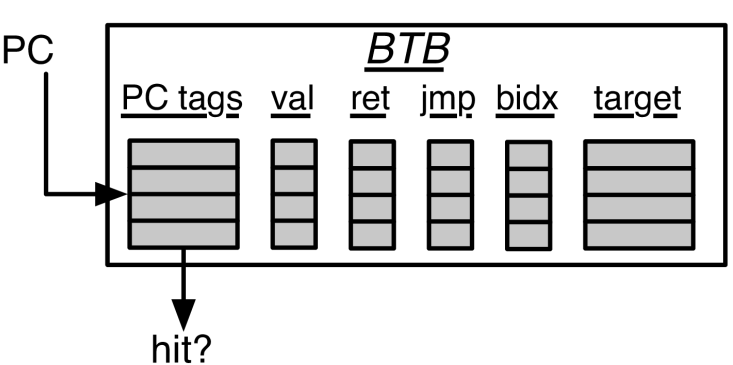
\includegraphics[width=0.5\linewidth]{BTB}
			\bicaption{BTB结构示意图。\citep{BOOMDoc2018}图3.2.}{BTB Unit Structure. Figure 3.2 of \citep{BOOMDoc2018}.}
			\label{fig:BTB}
		\end{figure}
	
		\textbf{返回地址栈(RAS)},用来预测函数调用的返回。寄存器类的跳转指令非常难以预测,因为寄存器的值是不固定的。函数调用后返回的地址虽然也是从寄存器读取的,但是却极具规律性,就等于调用该函数的指令的PC值加4,因此很好预测。而且函数的调用可以用栈来完全的刻画,所以预测器只需检测到函数调用的时候把调用函数的指令$ PC+4 $就压入栈中,等检测到函数返回的时候再弹出栈,就能很好的预测对绝大多数函数调用的情况。
		
		\textbf{分支预测器(BPD)},专门针对分支指令的优化,每一项只存储两位饱和计数器来预测跳或者不跳的跳转方向,所以必须要在知道是跳转指令以及跳转指令结果的情况下才能使用。这样,BPD可以和BTB一起并行查找,当BTB得到跳转地址以及是否命中的信息的时候,BPD刚好能够得到跳转的方向;或者BPD等到指令取回开始译码并算得目标地址的时候给出跳转方向。由于每一项的位数很小只有两位,所以项数可以做的很大,如1024项。这样就可以配合着10-bit的全局跳转历史通过哈希算法如gshare得到对于BPD的索引号索引BPD表得到跳转方向的信息。
		
		见图\ref{fig:boom_ftend},展示了前端各个预测单元的交互方式和流水线的组织形式。可以看到指令在F2阶段取回,被译码并计算得到目标地址,然后在F3阶段给出指令重定向的信息。这样能够给哈希算法整整一个周期的时间计算。BTB的组织形式可以是多样的,比如参考cache的设计采用多路组相连的形式而不一定要采用全相连的形式,这样可以节约电路的时序。
		
		还有一个模块值得注意的是在图\ref{fig:boom_predictor}中最灰方框中展现的名为B-ROB的单元,这一是个只存放分支跳转指令的小型的重排序缓存,里面保存了非常重要的处理器状态的快照(Snapshot),用来在分支预测错误时候对处理器的状态进行恢复,这同样参考的是MIPS R10000。
		\item 重命名阶段的数据结构和操作都很大程度借鉴了MIPS R10000的做法,不做赘述。
		\item BOOMv2的发射队列采用了和MIPS R10000几乎相同的组织形式,一个16项的定点指令队列,一个16项的浮点指令队列和一个16项的访存指令队列,见图\ref{fig:boom_total}。采用的是移位队列的形式(collapsing queue)并采用级联的优先编码器(cascading priority encoder)去选择最早就绪的指令发射出去\citep{Celio:EECS-2017-157}。不过BOOM是可配置的,所以BOOM同样提供了另外一种R10000风格的无严格先后次序的发射,但这样会导致性能不佳。
		\item 访存单元。BOOM设计了3个队列,the Load Address Queue (LAQ), the Store Address Queue (SAQ), and the Store Data Queue (SDQ)\citep{BOOMDoc2018}. 在这个设计上与Alpha 21264类似。如示意图\ref{fig:LSU}所示,load和store的地址要做一个二选一,选择更老的指令对应的地址去做访存。
		\begin{figure}[!htbp]
			\centering
			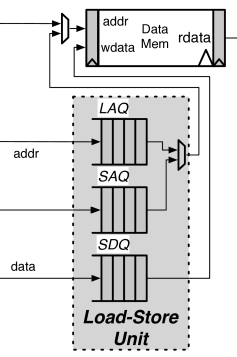
\includegraphics[angle=-90,width=0.5\linewidth]{boom_lsu_fig8_1}
			\bicaption{访存单元结构简化示意图。\citep{BOOMDoc2018}图8.1.}{Load-Store Unit simplified diagram. Figure 8.1 of \citep{BOOMDoc2018}.}
			\label{fig:LSU}
		\end{figure}
	\end{enumerate}

\section{研究方法与方案}
	纸上读来终觉浅,觉知此事要躬行。前面梳理了很多乱序多发射设计的相关工作与材料,最终还需要能转化为自己的设计。不过在设计之前,必须有一套开发验证的方法和平台,和一套成型的循序渐进由易到难的设计方案。这两个要素是开始设计必备的前提条件。
	
	\subsection{开发验证平台}
	
	本科学习期间采用的指令集是MIPS32,实验课上设计的单发射五级静态流水线处理器是基于龙芯提供的设计验证平台。设计中经历的步骤程序有:\textbf{step1}: 仿真时与龙芯提供的标准CPU loogson132生成(打印)的写回级trace对自动化的逐拍比对$ \Rightarrow $\textbf{step2}: 若比对出现不同则停止仿真,通过看波形找到产生不同写回信息的原因,并修正之$ \Rightarrow $如此循环往复直到仿真调通$ \Rightarrow $\textbf{step3}: 之后再用Vivado的集成化工具综合布局布线$ \Rightarrow $\textbf{step4}: 最后生成bitstream --- 可以配置FPGA的格式文件用JTAG线下载至Xilinx公司的FPGA上,产生物理上预期的效果就算设计完成。需要注意的是为了简化,课上实验中的内存是使用板卡上的SRAM模拟的,并不是真正的内存。
	
	但是这样一套自己比较熟悉的平台,却很难将RISC-V移植进来。没有现成的可以用来比对的标准trace;Chisel代码本身不支持波形调试,需要转化为低级的Verilog然后用仿真工具才能看波形,但是由Chisel转换而来的Verilog文件已经不是人可以阅读的形式了,有点像综合出来的网表格式。所以原来的平台并不奏效。
	
	很自然会想到在RISC-V开源处理器仓库中有没有可以略加修改便可使用的设计验证平台,于是尝试着阅读了Rocket和BOOM的说明文档及其代码。BOOM外围的很多代码是复用Rocket的,也就意味着存在着一种可能性 --- 区分出BOOM处理器自身和复用的Rocket代码,找到两者之间的接口,然后把BOOM替换为自主设计的处理器核心。但是不得不说,阅读代码的过程非常痛苦。首先BOOM和Rocket都已经是达到工业级别的颇为成熟的大工程了,里面的文件众多,每个文件中又有不同的类,而且这些类之间又有着非常复杂的交互关系。其次这些处理器的设计者和Chisel编译器的设计者属于一个团队,里面灵活使用到了Chisel和Scala中一些高级的语言特性来更为简洁,扩展性更强的描述电路,但是这些特性却是初学者一时很难理解的障碍。加之本设计的任务并不是在BOOM的基础上加些模块或者特性,也不是修改BOOM来达到性能的提高(再者说,这样难免有抄袭之嫌),任务在于自主设计出一款和BOOM一样完整的处理器的内核。所以如果需要和BOOM一样复用Rocket的外围代码,然后去跑仿真验证,就必须清楚的了解每一个细节,这一个熟悉的过程最少也需要几个月的时间,时间上来不及不允许。
	
	虽然BOOM和Rocket太过复杂驾驭不了,但是伯克利分校体系结构课程的教学用的是RISC-V,那么他们的实验就一定采用的是适合初学者的设计验证平台。果然,在伯克利分校CS152课程的网页上找到了他们实验平台,验证了这个思路是可行的。如今,这个实验的平台以及几个简单的能够在平台上运行的处理器核已经作为伯克利分校主要仓库目录列表ucb-bar中的\href{https://github.com/ucb-bar/riscv-sodor}{riscv-sodor仓库}开源了。同时还有一个\href{https://gitter.im/librecores/riscv-sodor}{论坛社区}(\url{https://gitter.im/librecores/riscv-sodor})。里面有很多初学者去提问,同时有包括RISC-V开发者在内的专家和热心的研究个体来答疑。所以对平台存在的疑问和漏洞都能在社区里提问,而经常浏览也能够学到很多初学者遇到的问题的原因以及背后的平台运行机制。其机制可以简化地用图\ref{fig:platform}来概括。
	\begin{figure}[!htbp]
		\centering
		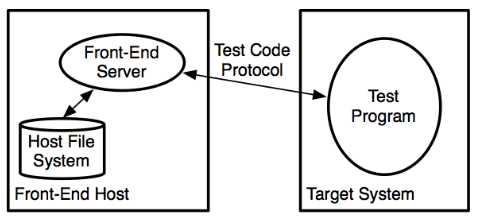
\includegraphics[width=0.5\linewidth]{platform}
		\bicaption{测试环境。前端服务器将RISC-V二进制文件加载到主机的文件系统中,启动目标系统的模拟器,发送RISC-V二进制代码到目标模拟器填充入模拟的处理器指令内存中。一旦前端服务器完成发送测试代码后,服务器重启目标处理器然后目标处理器就可以始从固定的地址开始执行程序。\citep{lab1}图2.}{The Testing Environment. The front-end server (fesvr) loads the RISC-V binary from the Host file system, starts the Target system simulator, and sends the RISC-V binary code to the Target simulator to populate the simulated processor’s instruction memory with the program. Once the fesvr finishes sending the test code, the fesvr resets the Target processor and the Target processor begins execution at a fixed address in the program. Figure 2 of \citep{lab1}.}
		\label{fig:platform}
	\end{figure}
	
	有了简单入门级的设计验证平台,再稍作修改,将原来糅杂在一个仓库中的处理器Chisel源代码和测试程序代码以及测试工具链如前端服务器软件和生成模拟器的C++库分离成两个相对独立的私有仓库,用git来管理,使得代码的编写工作变得更有条理。一级的文件目录结构如图\ref{fig:project}所示。同时,还对原来处理器源码的组织形式做了略微的调整,使得更符合JAVA的代码组织结构风格。另外,对于Makefile编译文件,也做了一些修改,使之符合自己的文件目录组织方式。
	\begin{figure}[!htbp]
		\centering
		\begin{subfigure}[b]{0.4\textwidth}
			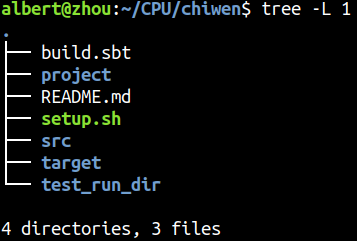
\includegraphics[width=\textwidth,height=4cm]{chiwen_L1}
			\caption{}
			\label{fig:chiwen_L1}
		\end{subfigure}\qquad%
		~%add desired spacing
		\begin{subfigure}[b]{0.4\textwidth}
			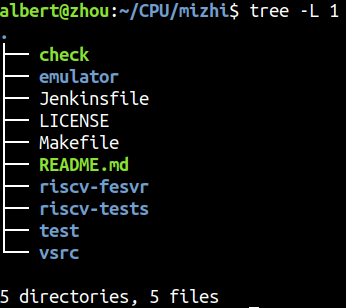
\includegraphics[width=\textwidth,height=4cm]{mizhi_L1}
			\caption{}
			\label{fig:mizhi_L1}
		\end{subfigure}
		\bicaption{毕业设计工程仓库。(a) 处理器Chisel源代码仓库。(b) 测试软件工具链和测试程序仓库。}{the repositories of the design. (a) The git repository which contains processors Chisel source, (b) The git repository which contains verification tool chain and test programs.}
		\label{fig:project}
	\end{figure}

	运行的流程大致为:
	\begin{itemize}
		\item 在\texttt{chiwen}目录下运行sbt,Scala的构建工具或者说是集成化的编译器(Chisel的编译器实际上是在sbt中加入前端的Chisel语法树分析,和后端的Chisel到Verilog的转化规则)。然后选择处理器的工程名,这样sbt就会产生一个处理器的C++精确到周期的描述。为了简化这一步骤,如图\ref{fig:chiwen_L1}编写了一个脚本,执行命令{\footnotesize \verb|terminal| -> \verb|./setup.sh processor_name|}即可。这个脚本最后会把生成的Verilog代码和Chisel的中间层表示Firrtl放到\texttt{mizhi}的\texttt{emulator}目录中以处理器名为目录名的目录下。
		\item 编译文件Makefile会用verilator软件将第一步得到的生成代码再生成和处理器对应的C++模拟器。
		\item 编译文件Makefile会调用RISC-V的前端服务器(fesvr)在文件系统中为第二步得到的C++二进制模拟器打开一个socket,然后将RISC-V的二进制文件文件传输到目标处理器去执行,见图\ref{fig:platform}.
		\item 在\texttt{mizhi}仓库里,已经提供了现成的测试程序包括指令功能测试和嵌入式benchmark程序性能测试(表\ref{tab:benchmark}列举了目前使用的八个程序),放在\texttt{riscv- tests}目录下。若要自己添加测试程序,可以放到test目录下,见图\ref{fig:mizhi_L1}. 程序的编译用RV32I的GCC工具链标准编译即可,这些具体的细节都掩藏在Makefile中,只需要输入命令{\footnotesize \verb|cd riscv-tests/isa| -> \verb|make|}生成指令测试二进制文件或者{\footnotesize \verb|cd riscv-tests/benchmarks| -> \verb|make|}生成性能测试的二进制文件。相应的,让目标处理器去仿真模拟执行只需要输入命令{\footnotesize \verb|make run-asm-tests|}或者{\footnotesize \verb|make run-bmarks-test|}就能运行指令功能测试或者benchmark性能测试。在Makefile中还提供了一些其他有用的命令。
		\item 最后如果通过,会在终端给出PASSED字样,否则就是FAILED来给出处理器的验证结果。大致的机理是Makefile会先用Spike,RISC-V的ISA级模拟器跑出一遍trace,然后比对处理器的输出结果。前端服务器(fesvr)也会通过debugIO通过访存来检测处理器的状态是否达到预期。不过存在着自动检测在FAILED时却给出PASSED的少见情况。针对这种情况,用python编写了一个脚本来比对待测试处理器产生的trace和Spike跑出的标准trace每一个周期的有效写回寄存器堆结果,或者也可以和sodor已经提供的几个简单处理器打印的trace做对比。这样就能严格保证处理器执行已有程序的正确性。
	\end{itemize}
	
	\subsection{设计方案}
	\begin{figure}[H]
		\centering
		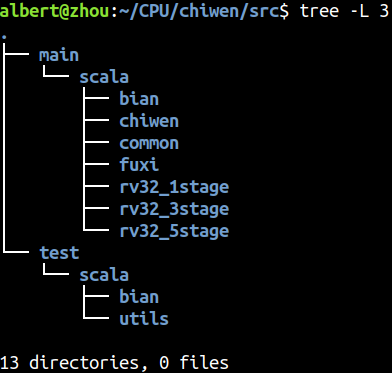
\includegraphics[width=0.4\linewidth]{chiwen_src_L3}
		\bicaption{目前为止已有的六款RISC-V RV32I处理器核。其中3款处理器CHIWEN(螭吻), FUXI, BIAN(狴犴)架构分别是自主设计的单发射五级静态流水线,双发射五级静态流水型, 和双发射乱序流水。另外3款rv32\_1stage, rv32\_3stage, rv32\_5stage是\href{https://github.com/ucb-bar/riscv-sodor}{riscv-sodor}提供的单周期、单发射三级静态流水线和单发射五级静态流水线处理器。common子目录包含了处理器共有的模块。}{The six Microprocessors based on RISC-V RV32I isa so far. There are three processors are self designed, including CHIWEN(single-issue, five-stage pipeline processor), FUXI(dual-isse, five-stage pipeline processor) and BIAN(two-wide superscalar processor with out-of-order). Other three simple processors are provided by \href{https://github.com/ucb-bar/riscv-sodor}{riscv-sodor}, with single cycle, three-stage and five stage single-issue architecture separately. \texttt{common} subdirectory contains common modules shared with all processors.}
		\label{fig:chiwen_src}
	\end{figure}

	若直接进行双发射乱序的设计,会因为没有很好的设计着力点而变得步履维艰。所以制定出一套详细的从易到难循序渐进的方案显得非常重要。同时,Chisel对于自己来说是一门全新的语言,也需要用一些简单的任务来充分地熟悉。
	
	在riscv-sodor中已经提供的有三款简单的处理器,分别是单周期(rv32\_1stage)、单发射三级静态流水线(rv32\_1stage)和单发射五级静态流水线(rv32\_5stage)。将它们拷贝至自己的仓库的文代码目录中,参见图\ref{fig:chiwen_src}。这些简单的处理器除去CSR特权寄存器逻辑的设计之外,处理器核心仅仅只有500多行代码,代码非常简洁易读,尤其是其译码部分。处理器采用的结构是经典的数据通路和指令通路。但是事实上这样的设计模式不好,两个通路之间是强耦合的。在阅读rv32\_5stage的过程中,也发现数据通路和控制通路的两个文件中相当有一部分代码是重复冗余的。为了可拓展性和控制复杂性的考虑,第一步是调整处理器的设计模式,采用和BOOM一致的前后端模式。重新对单发射五级流水修改后版本成为了处理器CHIWEN。同时,在修改的过程中,逐渐掌握了Chisel描述电路的常用写法。
		
	\begin{table}[!htbp]
		\bicaption{benchmark性能测试程序说明。除了coremark是自己添加的,其余的都是\href{https://github.com/riscv/riscv-tests}{riscv-tests}已经提供的}{The explanation of the set of benchmarks provided by the  \href{https://github.com/riscv/riscv-tests}{riscv-tests} repository except for coremark}
		\label{tab:benchmark}
		\centering
		\footnotesize% fontsize
		\setlength{\tabcolsep}{4pt}% column separation
		\renewcommand{\arraystretch}{1.2}%row space 
		\begin{tabular}{lcc}
			\hline
			名称 & 功能解释 & 备注 \\%inserts table 
			%\cline{2-9}% partial hline from column i to column j
			\hline
			coremark    & A synthetic embedded integer benchmark      & 合成的嵌入式整数程序 \\
			dhrystone   & A synthetic embedded integer benchmark.     & 合成的嵌入式整数程序 \\
			median 		& Performs a 1D three element median filter.  & 一维的中位数查找 \\
			multiply 	& A software implementation of multiply.      & 乘法的软件实现 \\
			qsort  		& Sorts an array of integers using quick sort. & 快速排序 \\
			rsort  		& Sorts an array of integers using radix sort. & 基数排序 \\
			towers 		& Solves the Towers of Hanoi puzzle recursively. & 汉诺塔 \\
			vvadd 		& Sums two arrays and writes into a third array. & 数组向量加法 \\
			\hline
		\end{tabular}
	\end{table}

	但是CHIWEN不是对rv32\_5stage简单重写。事实上rv32\_5stage运行benchmark(见表\ref{tab:benchmark})的统计结果显示,IPC普遍偏低。%TODO: add figures
	原因在于rv32\_5stage更没有转移猜测的机制,如果跳转指令的结果还没计算出来,就顺序往后取指。RISC-V没有延迟槽,而且在第三级计算出跳转目标和方向只有还会锁存一个周期再进入取指部件重定向取指。所以猜错一个分支跳转指令就会损失2个周期,这样IPC就不会高。所以第二个任务就是在CHIWEN的前端加入转移预测器,参考借鉴的是\citet{Celio:EECS-2017-157}中的BTB,BPD和RAS设计,做了一定简化。
	
	在riscv-sodor平台上取指和访存都是没有延迟的,默认是同步的逻辑。为了模拟真实的外围内存系统,写了一个带有随机性的延迟的中间桥放在处理器核和模拟的同步内存之间,并且采用的是AXI的标准接口。接着构建了容量为16KB的icache来缓存指令,提高在有延迟的取指环境中的处理器性能。但是出于简化设计的考虑,并没有构建dcache,访存没有延迟,为默认的同步时序。综上,前后端的模式的五级流水线架构,辅以转移预测器和icache构成了CHIWEN处理器。
	
	前后端模式的强大优势在于,从单发射的CHIWEN过渡到超标量宽度为2的双发射五级静态流水线FUXI的过程非常平稳,代码基本上能够复用,不用做大的修改,开发的时间和调试的时间都大大缩短了。
	\begin{itemize}
		\item 后端的修改较为简单,把CHIWEN的后端用Chisel里Vec的写法重新写一遍,构建出两条并行的后端执行流水线。然后解决两条并行指令之间的如写后写、写后读、同时为跳转指令、同时为访存指令、同时为特权态指令等冲突,将后一条指令停住一个周期做成串行执行。不光写起来简单,调试的时候也不会出现很多的bug。
		\item 前端的修改是重点,也是难点,涉及到icache和分支预测器都会做出调整修改。在后面设计实现的章节中做具体的介绍。
	\end{itemize}
	
	有了CHIWEN和FUXI这两代处理器核微结构的演进,然后才真正过渡到双发射乱序处理器BIAN的设计调试中。由于FUXI和BIAN都是超标量宽度为2的处理器,所以BIAN的前端可以完全复用FUXI的,而不需要单独重新设计。解决了前端的问题,最后就可以集中力量进行后端乱序发射的逻辑设计,前后端强大的优势再次得到了很好的体现。而且可以看的出来,最后高性能双发射乱序处理器的设计成功离不开由易到难循序渐进的正确设计路线。
	
	\subsection{调试手段}
	
	首先是模块级的调试验证。Verilog常用的做法是给待测模块写激励测试。这个激励测试相当于更大一级的测试激励模块,里面实例化了待测模块并构建有时钟时序和测试输入,然后通过仿真器人眼查看输出信号波形是否符合预期。如果真的编写过Verilog激励模块,就会真切的体会到编写过程的麻烦,不仅是因为语句的粒度太小,而且就算波形出现和预期不同的结果,也不能马上下待测模块有漏洞的结论,因为可能是激励模块写得有漏洞。在这样的背景下,Chisel语言自封闭的设计了一套基于Chisel和Scala编写模块验证的方式。它封装了\texttt{chisel3.iotesters.PeekPokeTester}的基类,编写待测模块的激励模块首先继承这个基类,待测模块输入端的赋值调用poke语句,输出端的验证可以用expect语句和预期值进行自动比对,也可以打印出来。同时,因为Scala是脚本语言,所以复杂的且带随机性的激励测试构造是便捷的。另外,最为关键的一点是,\texttt{chisel3.iotesters.PeekPokeTester}基类隐藏了时序的构造,因为电路的何时复位,时钟的频率多少,何时在上升沿对电路功能的仿真几乎没有影响。电路经过一个时钟周期的逻辑在Chisel的测试代码中用简单的\texttt{step(1)}就可以实现(括号中的1表示一个周期)。在\texttt{step(1)}之后的代码逻辑就会发生在\texttt{step(1)}之前代码逻辑的一个周期之后。Chisel的测试代码的组织形式和JAVA保持一致,见图\ref{fig:chiwen_src}中的test目录,这样方便管理和测试,特别是在IDE的编辑环境中。
	
	但是上述调试方法不再适用于将各个模块整合起来的整个系统。整个系统的激励输入还是要依赖于riscv-sodor的测试环境(见图\ref{fig:platform})。那么输出端又如何去验证呢?首先分析输出端核心的信号有哪些,最核心的是每一周期的寄存器堆写回信息加上store指令的内存写回的信息。如果这两方面的信息都符合预期就认为处理器的输出是正确的。这个预期可以由RISC-V的模拟器Spike得到的,也可以由经过验证的开源的处理器核如rv32\_5stage来得到。调试的流程为:\textbf{step1}: 写回信息打印出来以文本的形式存储$ \Rightarrow $\textbf{step2}: 用自己编写的一个自动对比的python脚本进行文本操作自动比对$ \Rightarrow $\textbf{step3}: 定位到开始出现不同的第一个周期$ \Rightarrow $\textbf{step4}: 在源代码中加入在这个周期之前一个窗口内打印与产生差错有关联的更多变量的代码$ \Rightarrow $\textbf{step5}: 重新编译执行$ \Rightarrow $\textbf{step6}: 通过分析文本中的调试信息来定位到源代码中的bug。
	
	这样调试方式虽然原始,如果需要重新加入打印信号,就需要重新编译执行。但是就其速度而言,因为不用做整个系统全信号的仿真模拟,仅仅是打印出是每一周期的写回信息以及一段窗口内的详细的相关变量信号而已,就算加上重新编译和执行的时间,也比波形图仿真更快。另外,由于设计的时候先采用了较为彻底的模块级验证,等到整合为完整系统时,bug数量大大降低了,而且基本集中在各个模块交互的逻辑上。同时,文本的优势在于可以灵活地编写一些文本操作的脚本做自动化的分析,这恰恰是波形所不具备的。比如需要得到某一周期执行级具体的指令,波形图上只能显示一个32位的数值,转化需要人工手动。但是文本就可以用一个脚本来自动转化。还有例如分析分支跳转预测正确率的过程中需要统计精确到不同跳转指令的误预测率时或者某一周期窗口内的跳转行为以及预测行为时,文本+脚本分析的手段都要明显优于波形图调试。
	
	正是采用了这种调试手段,从最开始的调试方式摸索阶段,用两周时间调通了带转移预测器的CHIWEN处理器,并且预测器的行为符合预期;再到用一周时间调通FUXI的前端,加上三天调通FUXI的后端;最后到用两周的时间(一周进行模块级的调试验证,一周进行整合系统的调试验证)调通了整合到FUXI前端的BIAN的后端。调试的时间的减少使得在微结构的设计上的时间变得相对充裕。
\chapter{设计结果}\label{chap:design}
由于双发射乱序处理器的结构复杂,细节众多,不可能事无巨细交代清楚。所以在本章节中,强调在设计过程中不同考虑的分析取舍和突出微结构设计中的亮点。
\section{处理器框架}
这里的框架指的是一种比微结构更加抽象的解耦合模型 --- 前端(Frontend)、后端(Backend)模型。在章节\ref{subsec:BOOM}中分析BOOM时已经做过了初步的介绍。
\begin{enumerate}[label=(\alph*)]
	\item 前端: 提供稳定的指令流,具体来说就是从初始地址开始源源不断地取回指令提供给后端处理。
	\item 后端: 接受来自前端的指令,进行运算,最后写回寄存器堆或内存。
\end{enumerate}
这个模型的优势在归纳起来:
\begin{enumerate}[label=(\alph*)]
	\item 前端不需要关心后端指令执行的机制;后端也不需要在乎前端取指状态机的运转流程以及所采用的缓存策略。例如对于可被缓存区域的取指,可以利用cache提高取指效率,也可以不用。
	\item 连接两端之间接口的信号非常少而且清晰。屈指可数 --- 前端到后端方向有指令以及指令是否有效,指令所在的PC,以及下一条PC的转移猜测信息;后端向前端有对于指令流的反馈如取回的指令是不是由于流水线的繁忙而需要阻塞,分支跳转类指令和例外中断对于指令流的重定向信息,以及对于转移预测数据结构的反馈更新。
	\item 前后端的解耦合模型,清晰的接口对于功能的调试、性能的调优也大有助益。
\end{enumerate}
%However, the kill signal is delayed a cycle for critical path reasons. BOOM的做法和我的类似
%BOOM (currently) does not rename any of the CSRs, and in addition to the potential side-effects caused by reading or writing a CSR, BOOM will only execute a CSR instruction non-speculatively. 
\section{处理器高性能因素考量}
衡量高性能的通用处理器有两个维度:频率(时钟一周期经过的时间)和IPC(单位周期完成的指令数)。不同于IPC维度是硬指标,频率这个维度,不同的硬件实现(FPGA/ASIC),同一逻辑的不同写法,甚至不同的综合工具都会对其有较大的影响,一个比较客观的分析方法是计算从一个触发器的Q端到下一个触发器的D端之间最多的门级数(在设计的时候靠着经验进行大致的估算和衡量,但是由于扇入扇出的影响,会存在误差)。因为现阶段刚刚完成了处理器的设计,还未来得及在综合工具上对电路延迟以及能够达到的主频做分析和磨合,所以目前对于高性能的评价主要依据IPC的高低。

要做高性能,基于前后端模型可以非常清晰的解耦合为做到高性能的前端和做到高性能的后端。
	\subsection{高性能的前端}
	
	供应指令要快。这个快又可以继续细分用三个维度来衡量:
	\begin{enumerate}[label=(\alph*)]
		\item \textbf{能够取回来有效指令的周期占总周期的比重}。由于现代的处理器运算单元频率越来越快,存储器的频率就相对变慢。直接访问存储器要数十上百周期。优化的方法是引入高速缓存(cache),面积小频率快。
		\item \textbf{指令宽度}。每周期的指令条数,直观上来看,指令宽度越大,指令供应的越快。
		\item \textbf{指令的正确率}。例如在没有延迟槽设计的ISA下的较为简单的指令宽度为1的单发射五级静态流水线结构中,当跳转指令还没有运算出来跳转的方向和地址时,若阻塞前端会白白浪费周期数。所以一般会采用各种预测投机策略来续上指令流。对于结构越复杂,缓存指令数越多的后端,对指令正确率的要求也就越来越高。
	\end{enumerate}

	对照这三个维度,同时考虑频率时序的优劣,就有很多权衡考虑。
	
	首先来看第一个维度。cache做多少大,多少路,要有多少个cache行,每个cache行要长度多少。cache的大小首要考虑的是ISA和操作系统对于分页大小的规定,对于RISC-V来说是固定4KB (参见章节\ref{subsec:ISA})。所以如果cache每路的容量大于4KB,不是实地址低位索引就会有顶着色的问题。但是若采用实地址索引,对于TLB的逻辑将是一个极大的挑战。虚地址要先经过TLB转化为实地址再去索引cache,若做成一个周期时序会紧张,若做成两级流水,由于跳转指令的存在,猜错的时候就会多浪费一个周期,效率反而会下降。一种比较简单的方案是cache单路的容量做成不超过4KB,这样,cache的索引号作为虚实地址的低位是一致的,换言之TLB转换和cache访问就可以达到并行,也即通过TLB CAM表查找得到实地址的高位锁存一拍再和与此时同步cache里读出的tag域做比较得到是否命中的信号。这样cache命中就只需要一个周期。但是代价是cache的容量太小,运行像dhrystone(见表\ref{tab:benchmark})这样指令范围大于4KB的程序,取指回来有效指令占比较低。出于增大容量的考虑,在毕业设计的CPU中准备采用四路的设计,每一路是4KB大小,这样总共就有16KB的容量。另外,cache行的的长度为64 Byte,可以存放16条指令。
	
	与cache不同,其他两个维度都与后端有着比较紧密的关联。对于指令宽度,如果前端是两条指令的宽度,后端做单发射流水线就不合适,指令供应的过快而后端消化不掉就会导致流水线阻塞,所以执行单元相应的至少需要两套。其次指令的宽度也不是越大越好,原因有如下几点:
	\begin{enumerate}[label=(\alph*)]
		\item 宽度大,会增大前端的逻辑复杂度,同一周期的各个指令非常容易出现前后数据相关、控制相关的问题。
		\item 面向内存的接口宽度仍为一条指令,所以一旦出现cache miss就会有大量的空泡产生
		\item 对转移猜测器产生了巨大的压力,每一周期对宽度内的每一个PC都要做预测,再根据预测的结果,前面指令无效掉后面指令,整个过程电路的延迟很大。而且不光延迟大,取指的效率也不会呈现出正相关。
	\end{enumerate}
	
	最后是指令的正确性。前文提到,后端的结构越复杂,级数越多,缓存的指令越多,如果还支持乱序,那么对于指令的正确性要求越高。一方面是级数越多,跳转指令从取指到执行的周期越长,如果猜错,损失的周期数就越多。换言之提高转移预测的准确性对乱序的提升会比顺序的显著。另外一方面,对转移猜测而言,结构越复杂的后端意味着前端可以有更多的周期进行分级的预测并矫正上游流水级的预测结果,使之更准确。例如乱序处理器一般在第三级做重命名以及分配物理寄存器而来不及执行,那么这个时候跳转结果依旧没有得到,还能够继续进行分支预测矫正。
	
	\subsection{高性能的后端}
	
	指令执行要快。这个``快''可以理解为尽可能少的阻塞前端指令的传送,也就是说不能因为少数的``刺头''指令拖累了整个CPU的指令通路,这里指的主要是访存类指令。同时通过目前已经设计出来的的单发射五级流水线CHIWEN,双发射五级流水线FUXI处理器运行几个小程序发现,在icache都命中、没有访存延迟而且分支预测正确率在97\%的情况下,CHIWEN的IPC可以达到0.99,FUXI的IPC最多只有1.33。也就是说当前端已经全速取指且指令正确率几乎为百分百的前提下,IPC与预期的2(与取指宽度成正比)相差很大。分析原因有如下几点:
	\begin{enumerate}[label=(\alph*)]
		\item 最大的原因首先是如果在同一周期的两条并行指令中第二条指令源操作数依赖于第一条指令的写回结果,就只能阻塞上游流水,串行执行。这种情况很常见。
		\item 访存指令的影响。其一,load-to-use的周期数代价更加大了;其二,由于内存访存依然是单端口的,就算添加了dcache,为了简单,也没有必要做成双端口。这样每一周期就只能允许一条指令去访存的,若遇到两条访存指令就必须拆成串行。
		\item 分支跳转类指令的影响。其一,前端存在两条并行指令只有第一条是有效的,第二条由于第一条被预测为跳转而被无效的情况。其二,两条跳转指令同时在执行级时,也要被拆成串行逐个计算跳转地址、比较预测信息,更新前端的预测数据结构并作出重定向前端指令流的抉择。
	\end{enumerate}

	如此一来,顺序执行的后端在超标量的前端面前已经达到了一个瓶颈,取指宽度为2的取指器,运行程序的IPC最高的性能也不会超过1.35。
	\begin{figure}[!htbp]
		\centering
	    \begin{subfigure}[b]{0.8\textwidth}
			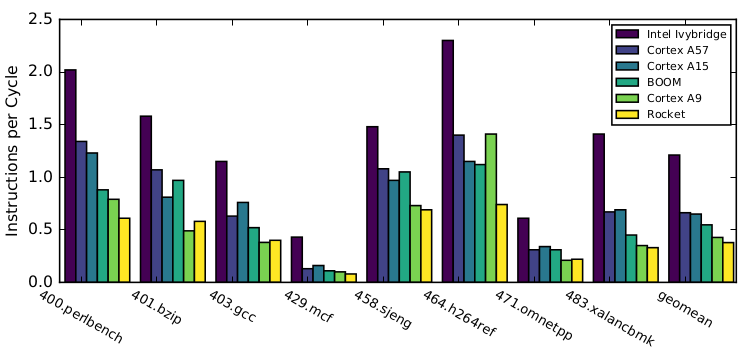
\includegraphics[width=\textwidth]{IPC_spec2006}
			\caption{}
			\label{fig:ipc_cmp_fig}
		\end{subfigure}
		\begin{subfigure}[b]{0.8\textwidth}
			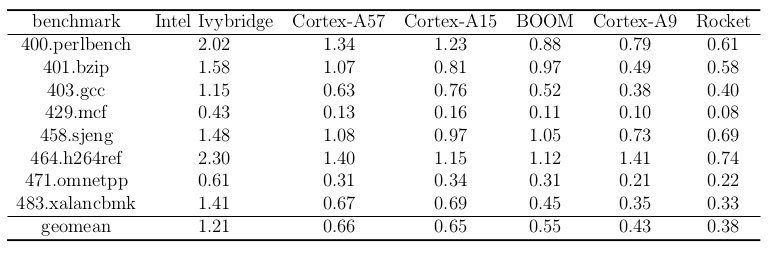
\includegraphics[width=\textwidth]{IPC_num}
			\caption{}
			\label{fig:ipc_cmp_tbl}
		\end{subfigure}
		\bicaption{SPECint2006 IPC不同IPC比较。(a) 图。\citep{Celio:EECS-2018-151}图3.7. (b) 表。\citep{Celio:EECS-2018-151}表3.6.}{Instruction-per-cycle comparison running SPECint2006. (a) The figure of instruction-per-cycle comparison running SPECint2006, Figure 3.7 of \citep{Celio:EECS-2018-151} (b) The table of instruction-per-cycle comparison running SPECint2006. Table 3.6 of \citep{Celio:EECS-2018-151}}
		\label{fig:ipc_cmp}
	\end{figure}

	虽然1.35已经是个不错的成绩,但是,是基于icache全部命中,没有访存延迟,而且转移预测器命中率达到97\%以上的前提下。在一般的情况下,可想而知连1都很难达到。对比图\ref{fig:ipc_cmp}中当前成熟处理器的性能,还有很大的性能提高空间。既然指令宽度为2的超标量顺序执行已经达到瓶颈,很自然地脑海中会浮现出三种方案:
	\begin{enumerate}[label=(\alph*)]
		\item 继续提高取指宽度,比如四条指令的超标量,后端继续做顺序。
		\item 不提高取指宽度, 因为对于指令宽度为2,前端供应指令的最大IPC可以达到1.8。计算方法为:每周期指令最多是2条,假设跳转指令占总指令的20\%,跳转指令在第一条位置的概率是50\%,跳转目标在第一条指令的概率是50\%,预测单元全部猜对,最后计算得到每周期正确的指令为1.8条。从1.33到1.8还是有较大的提升空间,所以后端可以采用乱序微结构来做指令的动态调度。
		\item 即增加取指宽度,又把后端做成乱序。
	\end{enumerate}

	权衡三个方案: 第一个反而是最不切合实际的,换言之与高性能的目标背道而驰。宽度为4的取指器要在已有的取指器的基础上改成4条指令宽度,由前面的分析,电路逻辑复杂,时序不好,对转移猜测极不友好。其次,从FUXI的IPC瓶颈的分析中,可以看出,真正的瓶颈不在于前端而在于顺序执行的后端。那么第三个方案呢,也不切合实际,主要是因为目前,是从来没有设计过乱序处理器的新人,水平有限。比较之下,第二个方案是最合适的。

综上分析,最后毕业设计的处理器核心具体的结构就是取指宽度为2的前端匹配上乱序执行结构的后端。

\section{中间层的引入}\label{subsec:middle_end}
事实上,前后端的设计思想最初应该是借鉴于编译原理的。编译原理作为计算机领域一门成熟学科,就是通过前后端的设计方法学来降低编译器设计的复杂度。类比于只采用前后端模型的简单编译器,对于简单的顺序执行的五级流水,前后端的划分也是足够的。但是为了做代码优化,编译原理专门提出了中间表示层的概念,依托清晰的结构化设计,再一次的有效地控制了问题的复杂度。而这一思路同样可以借鉴在结构上比顺序更复杂的乱序处理器的设计上。事实上,在乱序的处理器中,要从顺序的前端变化到乱序后端,最后再从乱序的执行变回顺序的提交,恰好需要有这么一个像中间桥梁一样的中间层的存在。

\section{处理器的状态}\label{subsec:cpu_state}
章节\ref{subsec:middle_end}中提到了引入中间层的必要性。而如果用一句话来概括中间层的作用,那就是管理处理器状态的变化。那么什么是处理器的状态。指令和访存的数据是外部来的激励,算不上是处理器的内部状态。所以只有PC值,32项数据寄存器值能算是处理器状态。站在更高的视角来看,所有处理器的物理数据结构,外来的指令数据最后修改的都只有这两类寄存器。而套用前后端的模型,前端管理PC,后端管理32项数据寄存器,中间层则是管理这些状态的变化。

\section{指令乱序调度和执行级别}\label{subsec:exe_hierarchy}
论及乱序指令调度,这样的机制虽然做到后面准备好的指令可以先于前面没有准备好的指令执行,但也不意味着要做到真正意义上的毫无差别调度最先准备好操作数的指令,哪怕这条指令距离最早未提交指令的64条开外。为了支持在这个例子里所说的远在64条开外的指令的乱序调度,所付出的硬件的代价对于效率的收益值不值得,是值得商榷的。但它一定不是一个好的设计思路,因为它没有体现出一种被体系结构所强调的思想 --- 层次化。就拿最为经典的存储结构来说,从处理器内部的寄存器堆,到一级高速缓存,二级高速缓存,共享缓存再到内存,硬盘,磁盘,好的设计是把越重要越常用的数据放在越快速的存储设备中的,而不会是因为寄存器堆很快速就去把寄存器堆做达到百兆的容量。换言之分清主次的层次化才是真正好的设计,处理器的设计亦是如此。所以,在毕业设计中特别强调,对指令调度乱序执行要有等级化、层次化的划分。

回想在顺序流水的设计中,其实同样有指令的执行等级划分,只不过做的很极端而同样不合理 --- 处在流水线越下游的指令执行级别越高,而且这种级别精确到每一条指令,只要下游早的指令没有执行完或者没有准备好操作数,上游的所有指令都不能执行。这就是顺序执行自带的而且无法改变的执行等级划分的通病。如果以这种角度来思考,乱序能带来了什么?带来的是可以打破这种僵硬的等级划分通病,带来的是可以自行定义执行等级的自由。当然这种自由是靠更多的硬件资源交换得来的,来之不易就不能随意挥霍。需要对执行等级的自定义深思熟虑,做到符合指令执行的规律,这样才会高效。

大方向的规律非常清晰,就是越早被取回的指令,执行等级越高,被优先执行的倾向越大,反之执行的等级越低。但是又不能像顺序一样走向极端。所以等级一定是按照指令新旧的梯队来划分的,如第一梯队,第二梯队等等,然后每一梯队里面包括了不止一条的若干条指令集合。就以BIAN处理器中具体体现出层级化的设计点举例来说,BIAN微结构上将指令的执行等级分为3级:
\begin{enumerate}[label=(\alph*)]
	\item \textbf{第一梯队的指令集合}:容量$2 + 2 + 2 + 4 = 10$条,参见图\ref{fig:bian_over1}。其中两条位于从重命名阶段到执行阶段的锁存器中,其他8条分别位于3个执行队列中。每条指令都存储住两个操作数,不需要再次读寄存器堆,侦听到写回总写结果立马可以在每个队列中选出最早的一条指令执行,分配有一个通用的ALU,和一个写回端口。相当于是两个输入三个输出的执行调度站,详细的调度策略参见章节\ref{subsec:execute_q}。
	\item \textbf{第二梯队的指令集合}:容量$ 9\times 2 = 18$条,是两个容量都为$ 8 + 1 $条指令的并行的发射队列,其中8条位于8项移位队列中,1条头部寄存器中,这样的设计时序会比直接9项的移位队列更好。队列中的每一项通过侦听前递信息判断操作数准备与否。位于队列中的指令会先移到头部;位于头部指令会和旁路过来的流水线二三级之间锁存器中的指令做二选一的逻辑,读寄存器堆获得源操作数,进入执行阶段。
	\item \textbf{第三梯队的指令集合}:容量$ 16\times 2 = 32$条,存储结构为循环队列,每一项可容纳两条指令。指令顺序出队列进入重命名阶段。容量最大,执行级别最低。
	\item 还有另外一类指令不好纳入这三个梯队中,由于功能特殊,而且是对外的操作,需要单独占有一个写回端口,这就是访存指令。这类指令对于处理器性能的影响很大,所以需要着重优化,我的设计中采用的是非常经典的LDQ和STQ分别存放load和store类指令的信号,参见图\ref{fig:ls_unit},目前的参数分别都是6项。同时为了提高访存密集型程序的性能,另外专门设计了一个可以同时存放load,store指令的load/store队列,里面只存放了很少量的关于访存指令的信息。作为比LDQ和STQ执行等级更低的存储单元以避免因为LDQ和STQ容量太小而导致频繁阻塞前端指令供应的情况。具体的设计考虑参见章节\ref{subsec:ls_queue};具体的运作机制参见章节\ref{subsec:ls_unit}。
\end{enumerate}
\subsection{总结}

如果保守估计在LDQ和STQ中共分担4条访存指令,那么乱序执行的指令总数可达$ 10+18+4 = 32 $条,在乱序执行的上游还可以有32条的顺序的指令缓存(第三梯队)。所以处理器中可以最多容纳64条指令,两条并行的发射队列(第二梯队),加上3条并行的执行队列(第一梯队)。另外,一共有3个ALU运算部件;寄存器堆有4个读端口,4个写端口,读写端口较少,特别是读端口数量是双发射架构中最少的。整个处理器架构如图\ref{fig:ls_unit},设计合理。
\begin{figure}[!htbp]
	\centering
	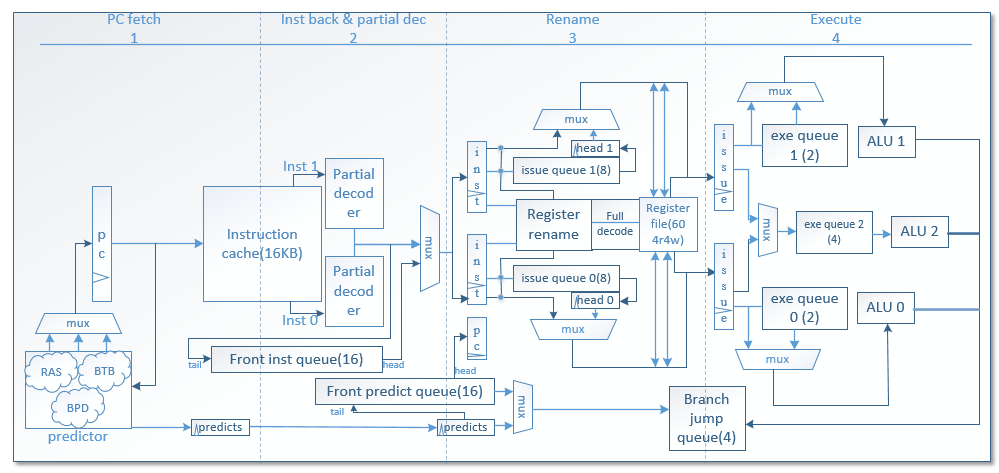
\includegraphics[width=\linewidth]{bian_overview}
	\bicaption{BIAN处理器整体框图,不包括访存单元}{Block diagram of BIAN processor (not include load-store unit.)}
	\label{fig:bian_over1}
\end{figure}

\begin{figure}[!htbp]
	\centering
	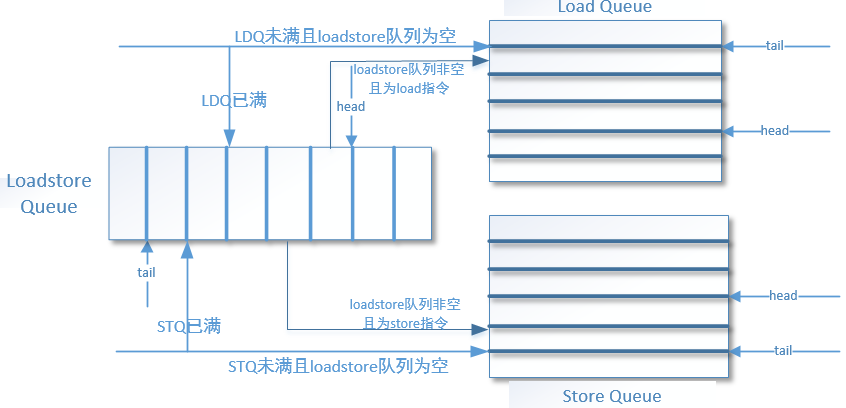
\includegraphics[width=\linewidth]{load_store_unit}
	\bicaption{BIAN处理器访存单元}{Block diagram of load-store unit in BIAN processor.}
	\label{fig:ls_unit}
\end{figure}

\section{流水线阶段划分}
%TODO 用了很多bypass的技巧
处理器流水级的划分如图\ref{fig:my_pipeline}:
\begin{figure}[!htbp]
	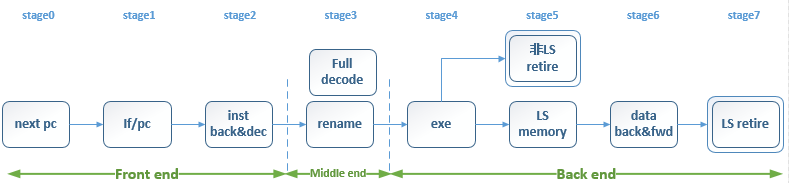
\includegraphics[width=\linewidth]{pipeline_stage}
	\bicaption{BIAN处理器的流水线示意图。}{the pipeline of BIAN processor.}
	\label{fig:my_pipeline}
\end{figure}
\begin{enumerate}[label=(\alph*)]
	\item 第0级 --- \textbf{next\_pc级}
	
	界定有没有这一级的标准是对于后端得到的跳转地址以及跳转使能信号,是直接送到pc级(稍后要介绍的第1级)向内存或icache发出PC,还是先送到锁存器锁存一个周期,再送到pc级。概括起来前一种做法是组合逻辑,后一种做法是时序逻辑。组合逻辑没有第0级,优势在于如果转移猜测错误,浪费的周期数会比时序逻辑要少一拍,最为极端的例子是在带有延迟槽的ISA如MIPS,最简单的单发射五级静态流水采用组合逻辑的方案从而不需要转移猜测。但是组合逻辑的劣势也是很明显的,就是时序不好,从后端计算出来直接跳转目标和有PC以及各级转移猜测的目标地址做多选,最后得到发出的PC值。pc级电路延迟很大,导致一方面访问icache的时序紧张,另外一方面如果要做转移猜测,那么PC值还要连到转移预测单元中得到下一周期PC值。这样就会把整个pc级撑得很大,对整个CPU的频率做高不利。所以本质上来讲,next\_pc级是为了缓解pc级的压力而增加的一级。
	\item 第1级 --- \textbf{if/pc级、取指级}
	
	发出PC从内存或者icache中取指,和经典的五级流水线保持一致。
	\item 第2级 --- \textbf{inst back \& dec级,译码级}
	
	这一级的名称兼容于经典的五级流水,原来的含义是指令在这一级被取回然后译码得到处理器内部操作微码。但是在BIAN处理器中,这一级只需做部分译码,得到一些简单的如是否是跳转指令的信息,从而减小这一级的电路延迟。再者,BIAN不会在接下来的第3级立刻执行指令,全译码放到第二级的需求不大。
	\item 第3级 --- \textbf{rename级、重命名级}
	
	这一级是BIAN处理器中至关重要的一级,承接着前端与后端,管理着后端的各种资源。从前端的角度来看,这一级还可以进行更加复杂策略的转移猜测;从后端的角度来看,这一级完成从逻辑寄存器到物理寄存器的转换和指令所需物理资源的分配。这里的物理资源有物理寄存器、内部指令标识符id号、也即reorder buffer的id号、访存队列、分支跳转队列、发射队列。读同步寄存器也在重命名级进行。
	\item 第4级 --- \textbf{execute级、执行级}
	
	在执行队列或者旁路过来的发射指令,选出3条准备就绪的指令在3个ALU中运算执行,如果是单周期ALU指令,写回寄存器堆;若是分支跳转指令发送到分支跳转单元;若是访存指令送到访存单元中。
	\item 第5级 --- \textbf{非LS retire级/LS memory级}

	乱序处理器流水级的划分从这级开始分化。单周期的ALU指令已经是retire级了,因为所需操作已经做完,在ROB中进行相应的提交操作就可以退出。但是对于访存类的指令,这一级是memory级,进行的操作是向内存发出访存地址和load请求。
	\item 第6级 --- \textbf{data back \& forward级}
	
	load所需的数据将在这一级被取回,同时做forward操作,将位于该load指令之前所有未写回内存,且与该load指令地址冲突的store指令的数据前递到load的数据中。成功加载到内存数据便可写回寄存器堆。
	\item 第7级 --- \textbf{LS retire级}
	
	对于load指令,在ROB中提交就可退出;对于store指令,当ROB队列的头部id号等于STQ的头部store指令id号时,将数据写回内存,并且移动ROB队列的头指针。退出处理器。这一过程中还会做backward操作 --- 检测位于该store指令之后是否有地址有冲突同时尚未做前递便已经将数据加载写回的load指令,若有,前端会以这条load指令的PC值为起点重新开始取指,做回滚操作。
\end{enumerate}
	\subsection{总结}
	访存指令从第0级到第7级完成提交退出,一共要经历8个周期,这是BIAN处理器指令流的最长路径。从前后端的模型来看,第0级到第2级的前3级流水属于前端(front end),第4级到第7级的后四级流水属于后端(back end),第3级单独成为一层 --- \textbf{中间层}(见章节\ref{subsec:middle_end})。
	
\section{前端的设计}
前端包括取指单元,转移预测单元和一级高速缓存。下面从这三个单元来剖析:
\subsection{取指单元}
从最简单的宽度为1的取指单元开始设计,代码如下:
\begin{scala} 
	/*一共有3个状态:
	* sWtAddrOK状态下等待地址握手成功
	* sWtInstOK状态下等待指令取回
	* sWtForward状态下等待后端接收取回的指令
	*/
	val sWtAddrOK :: sWtInstOK :: sWtForward :: Nil = Enum(3)
	val state = RegInit(sWtAddrOK) //取指单元的初始状态
	switch (state) {
		is (sWtAddrOK) { //在sWtAddrOK状态下
			//如果地址握手成功,切换到sWtInstOK状态
			when(addr_ready) { state := sWtInstOK }
		}
		is (sWtInstOK) { //在sWtInstOK状态下
			//若外界发送的指令有效,意味着指令被顺利取回
			when(inst.valid) {
				when(io.forward || inst_kill) { //被接收或者被取消,判断地址是否握手成功进入相应的状态
					state := Mux(addr_ready, sWtInstOK, sWtAddrOK)
				}.elsewhen(io.dec_kill) { //如果被流水线下游取消掉取回来的指令,切换到sWtAddrOK重新开始地址握手 
					state := sWtAddrOK 
				}.otherwise { //如果后端暂时无法接收,切换到sWtForward状态
					state := sWtForward 
				}
			}
		}
		is (sWtForward) { //在sWtForward状态下
			when(io.forward) { //被接收,判断地址是否握手成功进入相应的状态
				state := Mux(addr_ready, sWtInstOK, sWtAddrOK)
			}.elsewhen(io.dec_kill) { //如果被流水线下游取消掉取回来的指令,切换到sWtAddrOK重新开始地址握手
				state := sWtAddrOK 
			}
	}	}
\end{scala}
上面的代码就是描述整个取指器行为的状态机,一共只有3个状态,非常的简洁清晰,可以用图\ref{fig:fsm_fetchi}来描述:
\begin{figure}[!htbp]
	\centering
	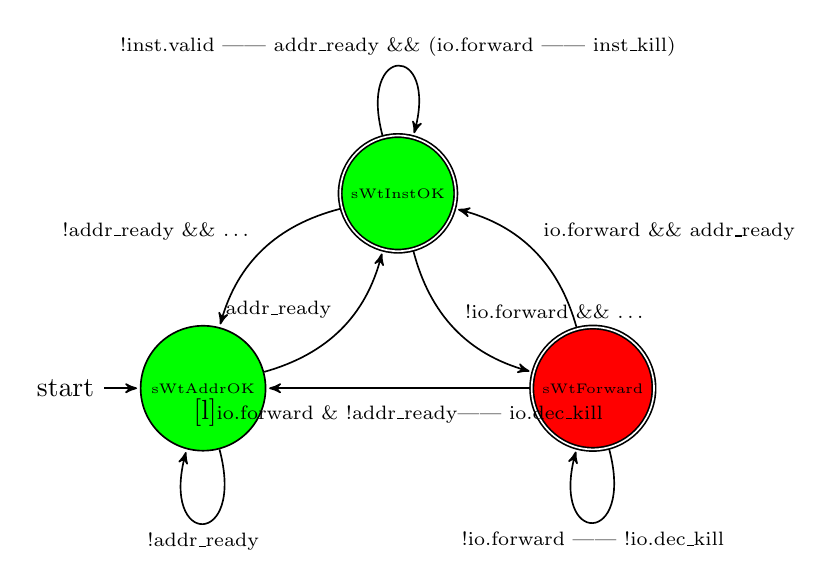
\begin{tikzpicture} [->,>=stealth',shorten >=1pt,auto,node distance=3.5cm,
	semithick]
	\node[state, accepting, fill=green](q0) {\tiny{sWtInstOK}};
	\node[state, below left of=q0, initial,fill=green] (q1) {\tiny{sWtAddrOK}};
	\node[state, accepting, below right of=q0,fill=red](q2) {\tiny{sWtForward}};
	
	\path
	(q1) edge[bend right] node{\scriptsize{addr\_ready}} (q0) 
	edge[loop below] node{\scriptsize{!addr\_ready}} ()
	
	(q0) edge[bend right] node[swap]{\scriptsize{!addr\_ready \&\& \dots}} (q1) edge[bend right] node{\scriptsize{!io.forward \&\& \dots}} (q2) edge[loop above] node{\scriptsize{!inst.valid || addr\_ready \&\& (io.forward || inst\_kill) }} ()
	
	(q2) edge[bend right] node[swap]{\scriptsize{io.forward \&\& addr\_ready}} (q0) edge node{\Longstack[l]{\scriptsize{io.forward \& !addr\_ready} \\ \scriptsize{|| io.dec\_kill}}} (q1)
	edge[loop below] node{\scriptsize{!io.forward || !io.dec\_kill}} ();
	\end{tikzpicture}
	\bicaption{取指单元的有限状态机。}{the FSM of FetchInst Unit.}
	\label{fig:fsm_fetchi}
\end{figure}

除了简洁的状态机模型,取指单元还做了两点设计:
\begin{enumerate}[label=(\alph*)]
	\item 在电路频率的考虑上,将所有从后端和内存传来的信号,都用锁存器锁存一个周期再去改变取指单元的状态,从而保证了取指单元的时序和外界独立。
	\item 为了配合图\ref{fig:fsm_fetchi}中的三个状态的状态机,取指的逻辑上有一个最为基本的限定 --- 取指的in-flight指令数最多为1。取指单元和icache都要相应地做成阻塞式,也即要等到正在访问内存或者icache的PC对应的指令被取回并被后端接收,才能够发出下一个PC取指请求。这种只能跟踪一条PC取指的方式,严格保证了取指的顺序性,同时取指单元的效率又不会有明显的损失。
\end{enumerate}

接下来是将取指单元的宽度从1提高为2,实现超标量。可是这个跨越并不简单。首先必须摆脱的误区是,由于内存的端口宽度是限定为1条指令32位的,所以如果直接访问内存,那么一个周期内取回的指令宽度仍然是1而不是2。故icache miss后burst传输是逐条指令传输回来的。宽度为2的情况只会出现在icache命中的情况下。这样,超标量的取指单元为了保证效率,显然不能等到可以两条指令同时从cache取回来的时机。Burst传输和uncacheable下直接访问内存的情况都要做到取回一条指令就立即发出一条指令。这样也可以理解为能够支持单宽度和双宽度之间的来回切换。得益于上述in-flight指令数最多为1的基本限定,双宽度的取指单元仅仅需要在原有的单宽带的基础上稍加修改。相比单宽度,双宽度有以下几个需要多考虑的逻辑:
\begin{enumerate}[label=(\alph*)]
	\item 超标量的两条指令是2对齐的,第一条指令一定是偶数PC,第二条一定是奇数PC。如果if/pc级发出偶数的pc,然而dec级由于cache miss再通过burst传输先传回了第一条偶数的指令,这时候可以不用顾及后端给出的forward接收信号,立马发出后一条的奇数PC取指。这个考虑使得无论再什么样的情况下,双宽度的取指效率都不会低于单宽度的取指效率。
	\item 指令流会有跳转,而且有一半的概率是在第一条指令的后面需要跳转(有预测单元给出),这种情况在BIAN的设计中被称为inst split,上述代码中用inst\_split变量来表示,如果第二条指令也取回来了,要取消掉。
	\item 当出现inst split的情况,而且预测单元给出的目标地址是奇数PC时,取指单元可以同样不用顾及后端的forward接收信号,直接发出跳转目标地址去取指。这样能进一步地继续提高取指效率。但是会存在子啊一个周期里被后端接收的指令不是地址连续的情况,这一点需要注意。
	\item 后端的forward接收信号变成了两位向量,使得并行的两条指令被后端接收变得独立。
\end{enumerate}

呈现的状态机代码如下:
\begin{scala}
	val sWtAddrOK :: sWtInstOK :: sWtForward :: Nil = Enum(3)
	val state = RegInit(sWtAddrOK)
	val inst_valid_orR: Bool = inst_valid.reduce(_||_)
	/*if_forward变量添加,是双宽度和单宽度之间最主要的不同
	* 表示的意义是当状态在sWtInstOK而且指令取回时,
	* 能够继续发送PC取指请求的集中不同的条件
	* 或表达式的最后一项的Mux多选逻辑参考
	* 前面双宽度需要多考虑逻辑的(a)(b)(c)部分
	*/
	val if_forward: Bool = io.forward(1) || inst_kill || Mux(inst_split, io.pc(conf.pcLSB).toBool, !inst_valid(1))

	switch (state) {
		is (sWtAddrOK) {
			when (addr_ready) { state := sWtInstOK }
		}
		is (sWtInstOK) {
			when(inst_valid_orR) {
				when(if_forward) { // almost the only difference
					state := Mux(addr_ready, sWtInstOK, sWtAddrOK)
				}.elsewhen (io.dec_kill) { state := sWtAddrOK
				}.otherwise { state := sWtForward }
			}
		}
		is (sWtForward) {
			when(io.forward(1)) {
				state := Mux(addr_ready, sWtInstOK, sWtAddrOK)
			}.elsewhen (io.dec_kill) { state := sWtAddrOK }
		}
	}
\end{scala}

\subsection{cache core设计}\label{subsec:cache_core}
数据和控制应该相互独立。这是为什么cache core和icache分开论述的原因。Core可以有不同的数据组织形式 --- 直接映射、全相连、多路组相连。同样,多路的时候可以有不同的替换算法。但这一切都与读写的逻辑无关,对外呈现的读写端口不变。只要求cache行的长度对外保持一致即可。将数据和控制逻辑解耦和,可以做到最大程度控制复杂度。另外一方面也可以做到逻辑的复用。比如icache和dcache对于读写的控制逻辑不一样,但是cache core的存储结构可以做到一致。虽然目前BIAN处理器仅是用一个16KB的直接映射组织结构来代替四路组向量每一路4KB的组织结构,但是由于数据和控制的分离,控制的逻辑无变动,对数据结构的修改其实并不困难。

\subsection{指令高速缓存}
Icache状态机的代码如下:
\begin{scala}
	val sLookUp :: sBurst :: sWriteBack :: Nil = Enum(3)
	val state = RegInit(sLookUp)
	switch (state) {
		is (sLookUp) {
			when (pc_miss) { state := sBurst
			}.otherwise { state := sLookUp
		}
		is (sBurst) {
			when (rlast && rvalid) { state := sWriteBack
			}.otherwise { state := sBurst }
		}
		is (sWriteBack) {
			when (pc_double_miss) { state := sBurst
			}.otherwise { state := sLookUp}
		}
	}
\end{scala}
\begin{figure}[!htbp]
	\centering
	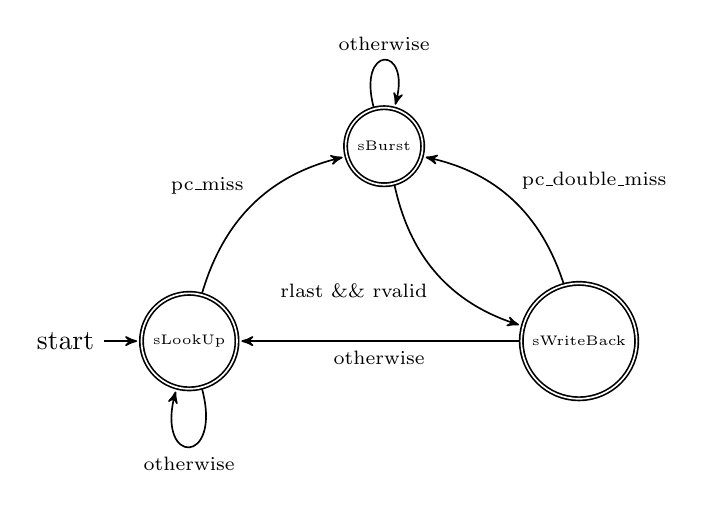
\begin{tikzpicture} [->,>=stealth',shorten >=1pt,auto,node distance=3.5cm,
	semithick]
	\node[state, accepting](q0) {\tiny{sBurst}};
	\node[state, below left of=q0, initial, accepting] (q1) {\tiny{sLookUp}};
	\node[state, below right of=q0, accepting](q2) {\tiny{sWriteBack}};
	
	\path
	(q1) edge[bend left] node{\scriptsize{pc\_miss}} (q0) 
	edge[loop below] node{\scriptsize{otherwise}} ()
	(q0) edge[bend right] node[swap]{\scriptsize{rlast \&\& rvalid}} (q2) 
	edge[loop above] node{\scriptsize{otherwise}} ()
	(q2) edge[bend right] node[swap]{\scriptsize{pc\_double\_miss}} (q0) 
	edge node{\scriptsize{otherwise}} (q1);
	\end{tikzpicture}
	\bicaption{Icache的有限状态机。}{the FSM of Icache.}
	\label{fig:fsm_icache}
\end{figure}

如图\ref{fig:fsm_icache},状态机一共有3个状态。sLookup阶段,在icache中以PC的低位为索引查PC对应的指令是否命中,如果出现miss了就进入sBurst状态进行burst传输。burst传输是AXI协议中的一种传输模式(但也不局限于AXI协议,很多高新能的总线协议中都有类似的模式),发出一个PC,能够取回这个PC所在的一段连续指令。比方说burst的长度设置为16,即使cache miss,在一段访问内存的延迟后,也有16个周期是有指令可以提供的,这样就能够大大降低访存延迟的代价。

BIAN的icache把burst传输长度设置为16,与cache行长度吻合。在AXI协议中burst有着两种基本的模式,一种是INCR,一种是SWAP。通俗来说INCR就是在以PC为起点,往后取一段指令,所以INCR发出的PC一般要指令长度对其。SWAP同样是以PC为起点,但是PC不要求是指令宽度中最前段的指令,可以是中间的某条指令,向后取指到达右边界后再循环到左边界直到取回来PC的前一条指令。icache采用的是INCR模式,因为其一取指有连续的倾向,而且在很大的情况下导致burst传输的pc都是cache行的第一条,虽然SWAP模式一定不会比INCR差,但是SWAP模式其实和INCR效率相差不大;另外,考虑到取值时序紧张,INCR模式对内对外都比SWAP模式友好。故最后采用的INCR模式。

回到状态机上,当状态是sBurst时,如果rlast和rvalid信号同时置上了,说明最后一条指令也被取回来了,状态就会跳到sWriteback状态。sWriteback状态下就是把取回来暂时用锁存器缓存的整个cache行写回章节\ref{subsec:cache_core}的存储结构中。为了提高效率,在burst传输阶段也是同步可以接收取回来的指令的,这样就会出现可能一个跳转出现第二次的PC在cache中的miss,这个时候整个取指单元就会因为in-flight取指数至多为1的基本限定而卡住动不了了。故在sWriteback状态下,如果检查到PC的二次miss就会直接进入sBurst传输阶段,从而提高效率。如果没有出现二次miss,那么就会又跳回sLookup状态。整个icache的行为简洁而高效。

\subsection{转移预测单元}
除了高速缓存技术,转移猜测也是高性能处理器的关键。与简单的流水线后端一遇到阻塞就要暂停前端取指不同,高性能的处理器一定是要做到后端遇到阻塞如访存数十拍的延迟时,还能允许前端继续投机地取指。来不及处理的指令将会被缓存在后端。按照转移指令在程序中15\%左右的占比,意味着指令流会在平均6$ \sim $8条之后可能重定向一次,如果没有转移猜测,一味的增加PC,等到前面的跳转指令被执行确认指令流需要重定向,那么后面的指令会被取消掉,体现不出指令缓存的作用,浪费存储面积。要真正发挥缓存指令的优势,就必须依赖转移猜测来提高缓存指令的正确性。转移预测可以分布在流水线的如下阶段:
\begin{enumerate}[label=(\alph*)]
	\item if/pc级要得到下一周期取指PC,此时还不知道PC对应的指令是不是跳转指令,唯一有用的信息是根据历史存储的从PC到目的地址的映射。但是PC有32位,靠RAM来索引不符合实际,剩下的方案只剩CAM表。代表性的数据结构是BTB,参见章节\ref{subsec:BOOM}。CAM表只能存少数的映射关系,比较理想的是32$ \sim $64个。在BIAN处理器中实现了用BHT和gshare算法辅助预测分支跳转方向,64项BTB映射表,能够存储64条分支跳转的目标地址。
	\item inst back级指令已经取回,但是整个周期剩余不了多少时间,最多只能根据局部译码检测到是函数返回指令选择RAS(参见\ref{subsec:BOOM})的栈顶地址重定向指令流。而在目前的BIAN处理器中,并没有实现在这一级基于RAS的转移预测,而是先锁存了一个周期,在rename级做。
	\item rename级中,对于简单的jal/j指令,可以直接由对应的PC和指令中的立即数域得到跳转地址并进行指令流重定向;对于branch类指令,虽然能够算出跳转地址,但尚不知道跳转方向。可以使用BHT和章节\ref{subsec:alpha}中提到的基于local历史和global历史的锦标赛预测机制来预测方向。目前,在BIAN的实现中,这一级仅仅做了jal/j指令以及对未在if/pc级未做预测的branch类指令的跳转。正在准备添加这段逻辑来提高预测率和处理器整体的性能。
\end{enumerate}

\subsection{预测单元优化}
在处理器的设计当中,有很多关于效率,时序,面积的权衡,这在预测单元的设计中得到了充分地体现。预测单元采用更加复杂的预测技术把预测正确率做到更高的同时,要付出更多的面积,更长的电路延迟和更大的功耗。在保证预测正确率的基础上,对于面积时序的优化也显得重要。下面突出在BTB结构中BIAN处理器所做的优化:

BTB原理简单,但是却是转移猜测中最为重要的一个部件,直接分担了程序跳转80\%左右的预测正确率。这个逻辑上简单的从pc到target的映射关系,值得好好的分析得到更好的物理实现,保证容量和正确率的同时降低面积和延迟的开销。
\begin{enumerate}
	\item 观察一:在映射关系中,无论是PC还是target的高位很少有变化,所以一个想法就是能不能把高位比如说高16位和低位比如低16位分开,做成两个表的映射。这样考虑到高位很少变动,高位的映射表项数就可以做的很小,比如4项(低位还是64项),如图\ref{fig:btb_opt1}。计算一下,采用这种的设计方案,总共占用的面积是$ 4\times16\times2 + 64\times16\times2 + 64\times2 = 2304 = 36\times 32\times 2 $ bits。最后加的$ 64\times2 $是在低位映射表中存储高位映射表的索引号所需要的面积,这个相当于36项32位PC映射到32位target的直接映射表。当然,如果是64位的ISA下,这种优势会更加明显。那么电路延迟如何呢?面积一样的情况下,两张CAM表的延迟不会比一张CAM表差,反而会因为面积减小,电路的布局布线上有优势。
	\begin{figure}[!htbp]
		\centering
		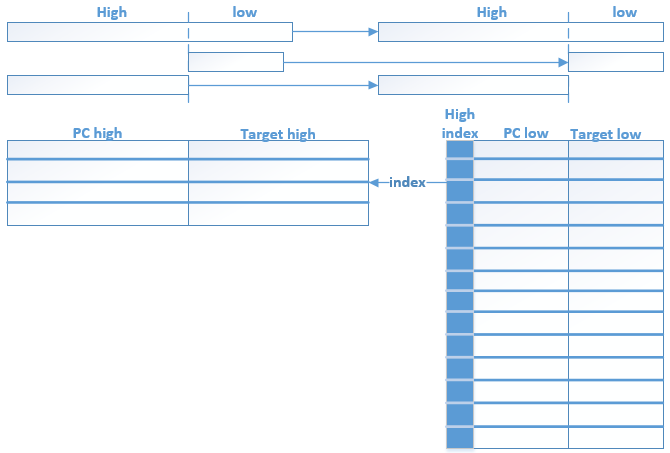
\includegraphics[width=0.6\linewidth]{btb1}
		\bicaption{观察一引出的物理数据结构的优化。左侧为高位映射表,右侧为低位映射表}{the physic data structure optimization by observation one. The left is the high bits map table, the right is the low bits map table.}
		\label{fig:btb_opt1}
	\end{figure}	
	\item 观察二:PC到target的映射中高位基本上都是一致的,也就是说程序的行为大多数都是在小范围内相对跳转。针对这一特点,在低位的映射表中再加1-bit的标志位,标记映射的高位是不是相等,如果高位相等就不需要占用高位映射表项,大大降低了高位映射表的替换率,从而提高了优化一数据结构的预测稳定性,如图\ref{fig:btb_opt2}。
	\begin{figure}[!htbp]
		\centering
		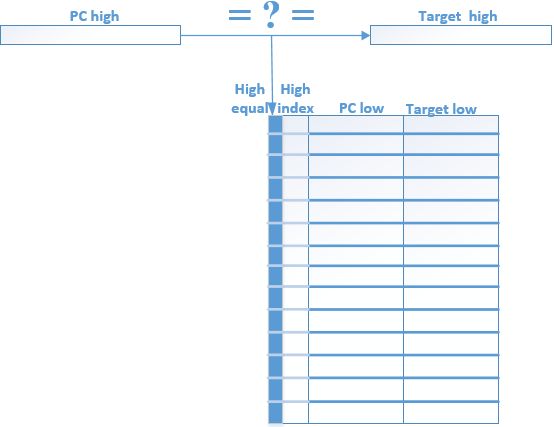
\includegraphics[width=0.6\linewidth]{btb2}
		\bicaption{观察二引出的物理数据结构的优化。只包含了低位映射表。}{the physic data structure optimization by observation two. Only include the low bits map table.}
		\label{fig:btb_opt2}
	\end{figure}
\end{enumerate}

\subsection{前端部件的整合}
上面讲述了前端的各个组件,这些组件整合起来构成了整个处理器BIAN的前端,如图\ref{fig:frontend}。
\begin{figure}[!htbp]
	\centering
	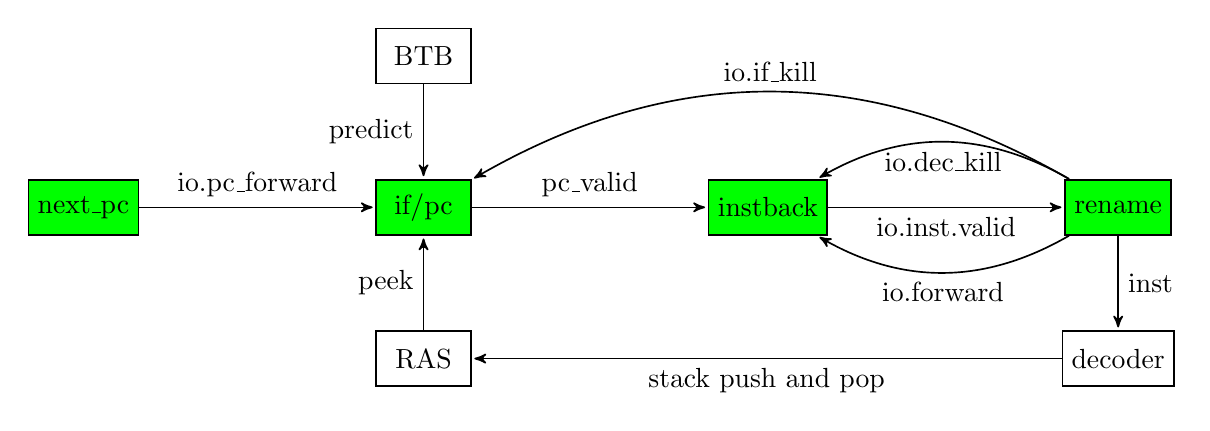
\begin{tikzpicture}[
	node distance = 12mm and 30mm,
	->,>=stealth',shorten >=1pt,semithick,
	box/.style = {rectangle, draw, fill=#1, 
		minimum width=12mm, minimum height=7mm}
	]
	
	\node (n1) [box=green] { next\_pc };
	\node (n2) [box=green,right=of n1] {if/pc};
	\node (n6) [box=white,below=of n2] {RAS};
	\node (n7) [box=white,above=of n2] {BTB};
	\node (n3) [box=green,right=of n2] {instback};
	\node (n4) [box=green,right=of n3] {rename};
	\node (n5) [box=white,below=of n4] {decoder};
	%
	\draw[->] (n1) to ["io.pc\_forward"] (n2);
	\draw[->] (n2) to ["pc\_valid"] (n3);
	\draw[->, swap] (n3) to ["io.inst.valid"] (n4);
	\draw[->, bend left] (n4) to ["io.forward"] (n3);
	\draw[->, bend right,swap] (n4) to ["io.if\_kill"](n2);
	\draw[->, bend right] (n4) to ["io.dec\_kill"] (n3);
	\draw[->] (n4) to ["inst"] (n5);
	\draw[->] (n5) to ["stack push and pop "] (n6);
	\draw[->] (n6) to ["peek"] (n2);
	\draw[->] (n7) to ["predict", swap] (n2);
	\end{tikzpicture} 
	\bicaption{处理器BIAN的前端流水线。}{the pipeline of frontend.}
	\label{fig:frontend}
\end{figure}

整个前端是一个三级流水,因为指令in-flight的请求至多为1的基本限定,十分简洁。主要体现在流水线的3大控制信号上:\texttt{io.pc\_forward}是控制取指PC从next\_pc级流向if/pc级的使能信号;\texttt{pc\_valid}是控制取指PC和BTB预测信息从if/pc级流向dec级的使能信号;\texttt{io.inst.valid}是控制取回指令和地址预测信息从dec级最后流向后端rename级的使能信号。这3级流水的阻塞与流通可以简单的解释为:首先最靠近后端的dec级如果在\texttt{io.inst.valid}和\texttt{io.forward}同时置上的时候,才能被后端接收,下一周期空出这一级,而if/pc级的信号要流向dec级须等dec级在下一周期能够被空出来,同理next\_pc级的信号要流向if/pc级须等if/pc级在下一周期能够被空出来。

相比于单宽度的前端,双宽度的前端还需要额外考虑两条并行的指令之间的干扰现象,具体来说是第一条指令对第二条指令的影响。在前端流水线的3级中:
\begin{enumerate}
	\item \textbf{if/pc级},虽然对外的取指端口是一个PC,但是这个时候对内的PC已经分化成奇偶两个。在BTB的结构中,如果第一条PC命中,并且方向为跳转,那么第二条的PC就会被无效掉。这一级的干扰现象被支取单元所解决。
	\item \textbf{inst back级},为了使得后端的逻辑简单化,通过局部译码,得到如果两条并行指令都是特权指令或者都是分支跳转指令时,就会阻塞该级流水,使两条指令串行发送给后端。
	\item \textbf{rename级},转移预测单元若在该级的第一条指令上纠正了流水线上游传输过来的预测信息,同样要将与之并行的第二条指令无效掉。
\end{enumerate}

\section{中间层的设计}

中间层承接着处理器的前端和后端。前端的前端指令队列、分支跳转预测队列的出口;后端的指令发射队列、分支跳转单元队列和访存队列的入口均位于中间层。中间层还专门负责管理处理器的状态变化与恢复,并能够按照每条指令的不同需求,精确地分配各个物理资源。是乱序处理器中最为重要的结构之一。

中间层涉及了很多部件单元。不过在论述每个具体部件之前,不妨先分析清楚承载这些功能单元的基本数据结构 --- 队列。

队列在电路中如图\ref{fig:queue}有两种实现形式:
\begin{enumerate}[label=(\alph*)]
	\item \textbf{循环队列},依靠着头尾两组指针来控制逻辑。称之为``组'',是由于考虑到同时入队列和同时出队列可能不止一项。入队列移动尾指针,出队列移动头指针。
	\item \textbf{移位队列},只需要依靠一个计数器来记录当前队列中有多少项即可。入队列从队列的尾部依靠计数器的指示进入;出队列项的后面诸项需要向前移位来填补出队列的空白。
\end{enumerate}
\begin{figure}[!htbp]
	\centering
	\begin{subfigure}[b]{0.45\textwidth}
		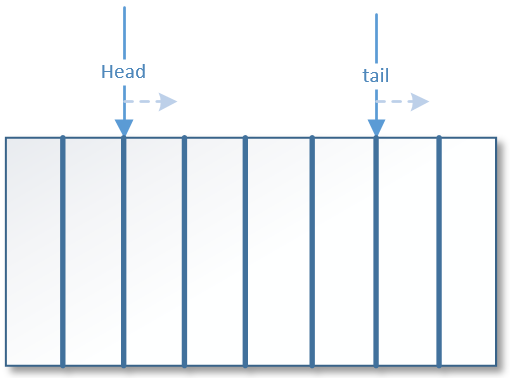
\includegraphics[width=\textwidth]{ring_queue}
		\caption{}
		\label{fig:ring_queue}
	\end{subfigure}
	~
	\begin{subfigure}[b]{0.45\textwidth}
		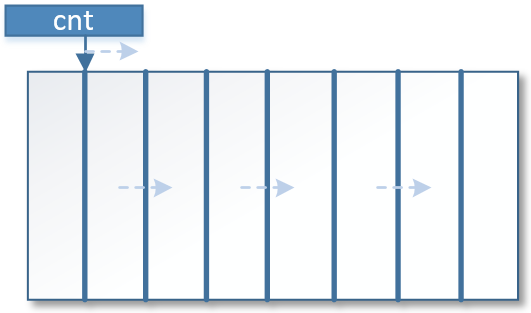
\includegraphics[width=\textwidth]{shift_queue}
		\caption{}
		\label{fig:shift_queue}
	\end{subfigure}
	\bicaption{两种类型的队列。(a) 循环队列,(b) 移位队列。}{Two types of queue. (a) Ring queue, (b) Shift queue.}
	\label{fig:queue}
\end{figure}

这两种不同的形式各有优势。循环队列对于出入队列的项数约束较松;移位队列入队列的项数约束较松,但是对于出队列的项数约束较严,一项是最为简洁的。项数一旦大于1,复杂度就会明显地提高,物理实现变得复杂,同时移位队列的功耗比循环队列大很多,因为移位队列平均1/2项数都会变移动,而循环队列只需要移动头尾指针。

但是循环队列并不适合承载乱序的逻辑,这是由其逻辑特性决定的,出队列项一定是头指针所指向的;与循环队列相反,移位队列非常适合承载乱序的逻辑,队列中的任何一项都可以出队列,留下的空位由后面项移位来补。同时,乱序中的多项同时可以出队,只选最早一项的逻辑,用移位队列来实现显得非常简单,只需要调用优先编码器,传入可以被发射的队列向量,最后按照优先级得到的独热码对应的就是应该出队列的最早一项。

但是移位队列的功耗毕竟太大,特别是每一项位数很大的时候。出于降功耗的考虑,对移位队列的结构做了优化如图\ref{fig:opt_shift_q}所示,只将能够决定出队列条件的最关键控制信号填入移位队列中,其他的数据信号则填入到数据表中,然后把该表项的索引同时填入移位队列中。出队列时再去索引数据表得到相关的数据。
\begin{figure}[!htbp]
	\centering
	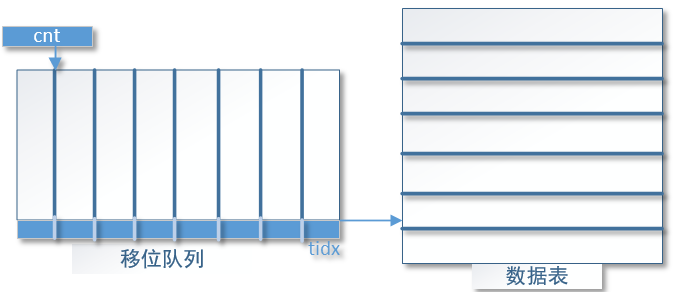
\includegraphics[width=0.7\linewidth]{opt_shift_queue}
	\bicaption{低功耗的优化,移位队列加数据表。}{shift queue plus data table, a optimization for saving energy.}
	\label{fig:opt_shift_q}
\end{figure}


整个中间层和后端就是用这两个最为基本的数据结构组合而成。一些复杂的操作流程,都可以规约为对队列的操作。以这样的角度去设计乱序多发射处理器,将会最大限度的控制复杂度,做到最大程度的简化。

\subsection{前端指令队列}\label{subsec:frontq}
除了有高速缓存的前端,高性能处理器在后端(包括中间层)中同样有一定数量的指令缓存,在BIAN的设计中被划分为了三个执行梯队(参见章节\ref{subsec:exe_hierarchy})。前端指令队列存储第三梯队的指令,入口位于inst back级,出口位于rename级。前端指令队列的结构如图\ref{fig:front_q},为循环队列的实现形式,所以第三梯队的指令是顺序被执行的。
\begin{figure}[!htbp]
	\centering
	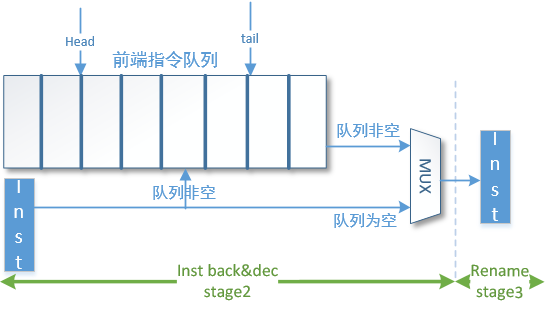
\includegraphics[width=0.7\linewidth]{front_inst_q}
	\bicaption{前端指令队列}{The queue storing for frontend instruction .}
	\label{fig:front_q}
\end{figure}

队列的每一项能够容纳两条指令,与取指器的宽度保持一致,让前端指令进入队列的逻辑保持简单。从取指单元取回来至少一条有效的指令,当后端没有剩余空间来接收时,会被压入该队列,从而不影响取指单元的继续取指。直到该队列满了,才会阻塞前端。BIAN中此队列有16项,容量一共是32条指令。执行benchmark程序时,几乎都为空的状态,主要用来隐藏16个周期的访存延迟。

\subsection{分支跳转预测队列}

从前端传来的不仅有指令,同时也有转移猜测的信息。直观上来讲,转移猜测的信息可以和指令一起存放在章节\ref{subsec:frontq}的前端队列中。但是由于前端指令队列的入口在inst back级,对于转移预测信息来说入队列的时机太早,所以不同于前端指令队列,分支的预测信息专门存放在分支预测队列中,在图\ref{fig:predict_q}流水线的中间部位。
\begin{figure}[!htbp]
	\centering
	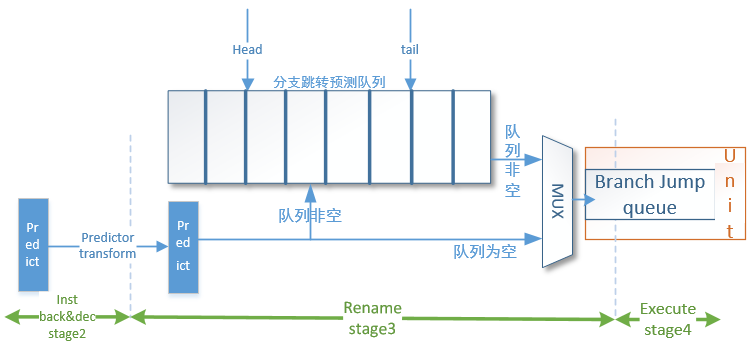
\includegraphics[width=0.8\linewidth]{branch_j_pipeline.png}
	\bicaption{分支跳转流水线}{The pipeline of branch jump instruction.}
	\label{fig:predict_q}
\end{figure}

该队列为循环队列,入口和出口均在rename级,所以预测信息可以等到rename级预测单元对预测信息做最后的修改再存入队列中。使用二选一的旁路来保证和出前端指令队列的指令是一一对应的。最后预测的信息会被写入分支跳转单元中的队列。因为前端在inst back级做了当两条并行指令同时为跳转指令将其串行化的逻辑,所以保证每一周期最多只有一条跳转指令。所以分支预测队列每一项的容量是一条指令的预测信息(通过二选一的逻辑选择出跳转指令的预测信息),这样,面积的开销减少一半。

\subsection{为什么不需要PC队列}

前端传来的不仅有指令和转移猜测信息,还有PC。直观来看,也应该有一个PC队列来存放每个指令所在的PC值。但是仔细一想,每一周期的PC其实也可以由分支预测队列存放的预测目标以及重定向使能信号推导出来。如果预测信息是错误的,也可以通过后端发送的取消信号重新更正PC。所以没有必要把pc存起来,这样,大大降低了处理器的面积开销。

\subsection{发射队列}

发射队列负责存储第二梯队的指令,结构如图\ref{fig:rename_inst_q},出口和入口都位于rename级,指令先进过重命名表,将逻辑寄存器号转换为物理寄存器号,并分配好资源后压入队列的尾部(为了做一个周期的优化,也做了旁路,当发射队列空时,不需要进入发射队列而可以直接选择发射)。不同于之前提到的各个队列,发射队列采用的是移位队列的实现方式(图\ref{fig:opt_shift_q}),这样可以支持乱序出队列,是实现乱序化最重要的一步。在细节上,移位队列每项的信息可以精简到两个物理寄存器号加上是否需要继续侦听的标志位和一个用来索引数据表的id号。这样,每项总共20-bit左右,其余的信息可以存储在数据表中,故移位逻辑的功耗得到了有效的控制。

由本章节开头对移位队列的分析,出队列项数为1是移位队列最合适的设置。但是双发射乱序要求发射项数为2,为了能够兼顾这矛盾的两点,采用的是两路并行的发射队列,事实上,图\ref{fig:rename_inst_q}中只给出了其中一路。每路每一周期都会从队列里弹出一项读寄存器堆然后发射到执行级。入队列也是严格按照物理的位置静态地每一路至多压入一项,处于时序的考虑不会采用动态分配的策略(也即如果第一路的队列满了,第二路队列未满,偶数PC的指令不会被动态压入第二路队列中)。这样的设定虽然会产生两路队列指令数量不平衡的情况,但是会由下游的执行队列来很大程度的缓解。
\begin{figure}[!htbp]
	\centering
	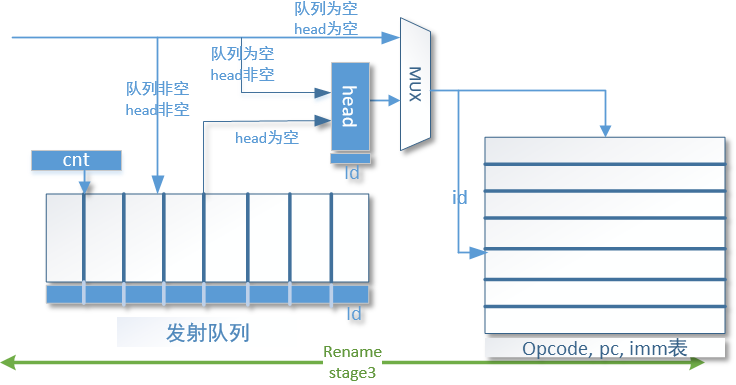
\includegraphics[width=0.8\linewidth]{rename_inst_q}
	\bicaption{单路发射队列}{One way of the inst issue queue}
	\label{fig:rename_inst_q}
\end{figure}

图\ref{fig:rename_inst_q}中的head是专门考虑电路时序的设计,这样发射的时候就不需要经过发射队列多选的过程。为了规整,移位队列主体为8项凑足2的幂次。若项数比8更多,侦听的电路效率就会下降。所以head的设计还增加了两条指令的容量。这样,两路发射队列总共的容量是18条指令。

在BIAN的发射队列设计中,有Alpha 21264,MIPS R10000和BOOM都没有的独特设计。从\ref{sec:meterial}的分析中看出,这三款处理器中,发射队列发射的指令必须是操作数都已经准备就绪的,当发射队列没有指令准备就绪时,这些处理器都没有打破僵局的机制和能力。但是BIAN处理器不同,发射队列依旧可以发射最早的指令,读取目前已经有效的操作数,然后发射到执行级,缓存入执行队列中(前提是执行队列未满),相当于是将指令的执行等级从第二级切换到了第一级。符合指令调度的直观。

\subsection{处理器状态控制单元}\label{subsec:state_unit}
在章节\ref{subsec:cpu_state}中,已经说明了什么是处理器的状态。处理器状态的正确变化是衡量处理器设计正确性的唯一标准,因此控制处理器状态变化的模块单元是处理器设计的重中之重。

无论是顺序处理器,超标量处理器,乱序处理器,本质上都是根据指令正确的改变处理器的状态。所以以一种更高的角度来看,高性能的处理器是能够高效的改变自身状态的机器(machine)。

乱序中最大的挑战在于处理器状态的维护和发生指令流发生错误的纠正。主要体现在三点上:
\begin{enumerate}[label=(\alph*)]
	\item 转移预测错误,要及时清除跳转指令后的错误指令流对处理器状态的改变,恢复至到跳转指令为止的处理器状态。
	\item 访存出现写后读冲突,但是后读的load指令先于写提交而且没来得及做数据前递,需要将状态恢复至到该load指令前面一条指令为止的处理器状态。前端重新从这条load指令起开始取指。这个在处理器设计的专业术语里叫做回滚。
	\item 例外和中断的发生。需要将状态恢复到中断例外指令之前的所有指令更新完的处理器状态。
\end{enumerate}

顺序执行的处理器,其状态是非常好维护的,因为指令都是顺序修改寄存器堆中寄存器值的,指令流出现错误也不会产生错误的处理器状态。但是乱序不一样,错误的指令流可以在未检测到之前对处理器状态做出改变。在目前的BIAN处理器设计中,实现的是RAM形式的重命名表,故处理器状态的恢复回溯也要以RAM重命名表为中心。下面是代码所描述的处理器状态的变量集合,以类的形式封装在一起。
\begin{scala}
	class State(val nEntry: Int) extends Bundle {
		val useing = UInt(nEntry.W)
		val usecnt = UInt(log2Ceil(nEntry+1).W)
		val maptb  = Vec(32, UInt(log2Ceil(nEntry).W))
		val rename = Vec(32, Bool())
	}
\end{scala}
	
基于RAM的重命名表在上述代码中是\texttt{maptb}变量,nEntry是物理寄存器堆的项数,所以$ log2Ceil(nEntry) $就是索引物理寄存器堆地址的位数。BIAN处理器设置了60项物理寄存器。其他变量的含义分别是:
\begin{enumerate}[label=(\alph*)]
	\item \texttt{useing}: 正在使用的物理寄存器分布向量,每一个物理寄存器占一位,1表示正在被使用,;0表示空闲,可以被分配。
	\item \texttt{usecnt}: 正在使用的物理寄存器计数器,产生分配物理寄存器的ready信号,比如需要分配一个物理寄存器需要条件usecnt < nEntry成立。
	\item \texttt{rename}: 逻辑寄存器号是否已经被映射到某一个物理寄存器号,如果是则为1,不是为0。含义是清晰的,用于写后写冲突中,后写的指令能够在指令提交时回收旧的物理寄存器。
\end{enumerate}

所以有了明确的状态刻画,需要有多少个\texttt{State}类只需要\texttt{new}出来即可。那么一共需要多少个\texttt{State}类呢?首先要有一个最新的状态,负责当前的重命名和物理寄存器号分配,这一个作为主要的\texttt{State}。其次为了精确的状态回溯,考虑要有状态的备份。回到上述提及的三种需要状态回溯的情况,可以分为两种不同的处理机制:第一种,发现指令流错误,马上撤销之后的指令流和处理器状态变化,发送重定向请求到前端;第二种,等到前面指令都已经顺序提交退出,再做发送重定向的请求,并撤销后续指令流和处理器状态变化。像转移预测错误因为比较频繁发生,所以一般做成第一种机制;而像回滚和中断例外,很罕见,可以做成第二种机制。BIAN处理器就是这么处理的。第二种机制需要有一个\texttt{State}备份记录至提交指令为止处理器的状态;第一种机制又可以有两种不同的做法,参见章节\ref{sec:meterial}中对Alpha 21264 (\ref{subsec:alpha})和MIPS R10000 (\ref{subsec:BOOM})的分析,在BIAN中采用的是MIPS R10000的做法,只针对每一条跳转指令做一个\texttt{State}备份。而在BIAN处理器中乱序部分最多支持四条分支跳转指令的投机,所以状态有四个备份用来回溯。代码如下:
\begin{scala}
	val latest = RegInit({ //当前用于重命名的最新的处理器映射状态
		val w = Wire(new State(nPhyAddr))
		w.maptb  := DontCare
		w.useing := 0.U
		w.usecnt := 0.U
		w.rename := VecInit(Seq.fill(32)(false.B))
		w
	})
	val commit = RegInit({ //是回滚和中断例外的状态备份
		val w = Wire(new State(nPhyAddr))
		w.maptb  := DontCare
		w.useing := 0.U
		w.usecnt := 0.U
		w.rename := VecInit(Seq.fill(32)(false.B))
		w
	})
	//nBrchjr = 4, 分别对应每一条投机执行的分支跳转指令的状态备份
	val backup = Reg(Vec(nBrchjr, new State(nPhyAddr)))
\end{scala}	

有了状态的描述,回溯恢复就是把相应要回溯的状态变量赋值给latest状态即可(省略复杂的细节),非常的简单直观。

除了基于重命名表的状态记录和回溯机制,作为处理器状态的主要控制单元,还有两大主要的功能:
\begin{enumerate}[label=(\alph*)]
	\item 指令id号的分配,载体是ROB,组织形式是循环队列,id号从尾指针顺序分配,从头指针顺序回收。
	\item 物理寄存号的分配。分配的时候在\texttt{latest}状态变量的\texttt{using}属性中,从左边找第一个1,从右边找第一个1,并行分配两个物理寄存器号。
\end{enumerate}

指令id号是标记处理器乱序部分顺序的唯一标识符。BIAN的分配的id号是5位的,对应于乱序部分最多可以in-flight 32条指令。

\subsection{分支跳转队列}

分支队列和访存队列就是面向后端的数据结构,分别在后面章节\ref{subsec:bj_unit}和\ref{subsec:ls_unit}中会详细说明设计中的亮点。

分支跳转队列的入口在中间层,说明是顺序分配资源进入队列,而不是不是执行时乱序分配的。原因很简单,因为分支跳转是控制相关的,带有顺序属性,在乱序中也要保持相对的顺序。采用的数据结构组织形式和发射队列类似,为移位队列,如图\ref{fig:bj_unit}。
\begin{figure}[!htbp]
	\centering
	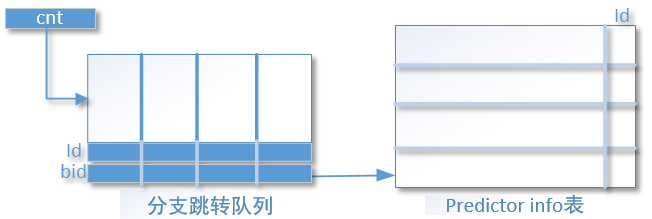
\includegraphics[width=0.8\linewidth]{branch_j_unit}
	\caption{分支跳转队列。}{The shift queue storing for branch and jump instruction.}
	\label{fig:bj_unit}
\end{figure}

\subsection{访存队列}\label{subsec:ls_queue}

解释两个和访存队列有关的问题:其一,直观来讲,访存指令并不是控制相关的,那么为什么访存单元队列的入口设置在中间层,要求顺序的时候分配资源呢?其二,从图\ref{fig:ls_unit}给出的访存队列数据组织结构中,为什么不和发射队列和分支队列一样采用的移位队列,而是用循环队列呢?

核心的原因在于:首先,对比普通寄存器数操作指令,写后写,写后读的冲突可以由重命名机制完美地解决,但是重命名机制却做不好访存指令的写后写,写后读冲突,因为访存的地址不是在rename级得到的,而是在乱序的执行级得到的。乱序执行是无法检测访存指令之间写后写,写后读的冲突。所以为了解决这个问题,这里就必须用队列的顺序分配来对保持访存指令之间的相对顺序。其次,因为store的写操作是对外的,所以已经超出了章节\ref{subsec:state_unit}中论述的处理器状态控制的范畴,要实现精确的状态恢复,store指令必须在LS commit级将数据顺序写回内存中,其顺序性需要有队列这样的first in first out的结构来保证。

队列类型不用移位队列而采用移位队列的原因在于:为了判读写后写,写后读的冲突,整个32位或者64位地址都将是关键信号,也要在移位队列中进行移位,如此一来功耗将会非常大。所以从功耗的开销和所获得的收益的角度来考虑,BIAN处理器做成6项循环LDQ和6项循环STQ,已经大概率的满足in-flight的32条指令中访存指令的存放需求。

\subsection{精确资源分配}
在中间层的设计过程当中,发现资源的精确分配逻辑非常复杂。资源的精确分配,指的是根据指令精确到对各个物理部件资源的不同需求和对应的各个物理部件单元剩余容量,做出资源分配。

这个逻辑的复杂性在于:
\begin{enumerate}[label=(\alph*)]
	\item 不同指令的需求是不一样的。有的指令有写寄存器的需求,所以需要分配物理寄存器;有的是跳转分支指令,在分支队列要分配项数;有的是访存指令,需要在访存队列中分配项数。
	\item 不同资源的剩余容量参差不齐,只要有一种资源指令有需求,但是无法分配,这条指令相关的其他指令都不能分配。
	\item 同一指令的需求是多样的,可能既需要物理寄存器,也需要访存队列
	\item 需要对两条并行的指令进行同时分配,第一条指令的分配情况会组合逻辑的作用于第二条指令发分配情况。所以并行的指令如果要实现精确分配物理资源就必须是串行的。
\end{enumerate}
\begin{table}[!htbp]
	\bicaption{中间层需分配资源列表。}{The list of resources in the Middle end.}
	\label{tab:resource}
	\centering
	\footnotesize% fontsize
	\setlength{\tabcolsep}{4pt}% column separation
	\renewcommand{\arraystretch}{1.2}%row space 
	\begin{tabular}{cc}
		\hline
		资源名称 & 备注 \\%inserts table 
		%\cline{2-9}% partial hline from column i to column j
		\hline
		指令标识符id   & 每条指令都必须分配,最多同时分配2项  \\
		物理寄存器号   & 有写寄存器的需求的指令分配,最多同时分配2项  \\
		发射队列entry & 每条指令都必须分配,每路队列最多分配1项  \\
		访存队列entry & 访存指令需要分配,最多分配2项 \\
		分支队列entry & 分支跳转指令除了jal类,最多分配2项 \\
		\hline
	\end{tabular}
\end{table}
\begin{figure}[!htbp]
	\centering
	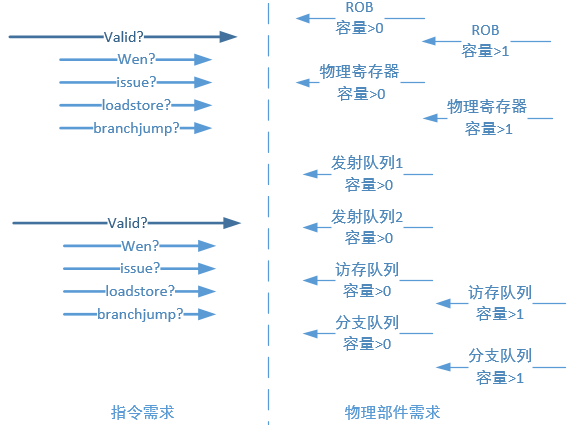
\includegraphics[width=0.7\linewidth]{issue_analysis.png}
	\bicaption{资源精确分配分析。}{analysis of precisely resources allocation.}
	\label{fig:issue_analysis}
\end{figure}

所以多发射宽度更高如四发射的很多处理器都采用了保守发射的逻辑来避免精确带来的复杂性。只要指令有效,就认为指令有所有的需求。换言之,在分配资源时只需要顾及指令是否有效即可。另外,在复杂处理器的设计中,由于各个部件单元的面积都很大,布局布线后的位置也会相隔较远,所以若采用精确发射走线延迟会很大。但是BIAN处理器后端面积不大,资源队列的项数较小,故走线延迟在可接受范围以内。另一方面,项数少就要采用精确分配的逻辑来节约使用。所以权衡之下,BIAN处理器中间层资源分配采用精确的方式,来提高资源的利用率和执行的效率。


BIAN处理器中间层需要分配的资源有五个,如表\ref{tab:resource}所示。
一方面是两条并行指令的各个需求以及是否有效,另外一方面是各个物理部件的容量信息,如图\ref{fig:issue_analysis}所示。

\section{后端的设计}
执行队列是完全属于后端的单元;分支跳转单元和访存单元除了队列入口在中间层外,部件的主体在后端。
\subsection{执行队列}\label{subsec:execute_q}

这个队列就是上文提及的执行等级的第一梯队,组织的格式同样是图9的移位队列,而且移位队列中entry的内容和发射队列保持一致,物理上就可以保证指令的相对顺序。缺点很明显 --- 面积开销很大,但是优点同样明显,执行快而且不需要读寄存器堆,将物理寄存器堆的读端口维持在4个,物理布局布线能够接受的水平。执行队列还有一个很重要的功能是及时平衡发射队列的指令数量。因为两个发射队列是独立平行的,每个队列只分别负责接收从前端送来的两条指令的有效的第一条和第二条。由于并不是每个周期的两个指令都是有效的,所以会导致发射队列指令数不平衡,影响到资源的利用率。依靠执行队列,当执行级两条指令同时因为操作数没有准备号被阻塞住时,接受来自含指令条数多的发射队列的那一条指令,从而起到平衡发射队列的作用。
\subsection{分支跳转部件}\label{subsec:bj_unit}
主体是分支跳转队列,对接着前端的转移预测器,构成了整个反馈回路的分支跳转系统。这一系统在高性能处理器的重要性仅次于访存系统。高性能的分支跳转系统在设计的时候有3大指标需要考虑:
\begin{enumerate}
	\item 高准确率  是设计的首要指标,90\%的准确率下处理器的IPC和95\%的准确率下的IPC都要相差很多。
	\item 低周期数  同样是设计中要考虑的重要指标。反馈周期的定义是从投机的取跳转指令的下一周期的指令开始,到跳转指令被执行能够发出重定向信号为止,一共需要经过的周期数。
	\item 低延迟,小面积,低功耗。
\end{enumerate}
而在分支队列的设计中,主要对应的指标就是低周期数。分支队列的结构如图13所示,目前的设计中有4项,也就是说乱序的32条指令中允许有4条分支,这四条分支能够把整个指令流分成5段,所以每段的平均长度在$6\sim7$之间,恰好也符合跳转分支指令在总指令中的平均占比。回到图13,会发现和图9的标准移位队列有些出入。主要体现在的地方是分支队列和分支信息表都多了id域(bid是需要的,因为要索引数据表)。移位队列要有id域是由于中间层就要分配,但是后端的执行是乱序的,执行完成回到分支队列就要用到cam查找去匹配到属于自己的那一项entry,然后再靠对应的bid来索引table得到相应的信息。理论上还存在着另外一种方案,就是ram查找,如果用ram,就必须在每一条指令都带上bid,比cam逻辑麻烦,而且分支跳转队列只有4项,算得上项数很少了。

table中的id域的作用同样是为了cam查找。这个id域是可以不要的,因为可以先通过cam索引移位队列得到对应的bid然后再去索引table。但是如果加上id域,就意味着两个结构的查找可以做到并行。这并行的考虑正是为了降低反馈周期数而专门设计的。反馈做到可以走组合逻辑路线的就不走时序逻辑路线。什么情况下可以用组合逻辑而又不影响CPU整体的延迟。仔细分析一下,除了jr类指令需要读取寄存器来进行运算,其他的分支跳转指令都是直接通过pc和指令中的立即数域进行符号拓展就可以得到跳转地址的,所以到中间层的时候跳转地址就能够被计算出来,顺势就可以存入分支表中。而且还需要注意的是像j类指令直接知道跳转地址和一定要跳的指令,是不会进入分支队列的,在risc-v中只有branch和jr两类指令会进入队列。在执行级,branch真正做的操作只有两个操作数的比较,工作量相对较少,所以就非常适合组合逻辑直接反馈;而jr类指令因为要算地址,所以先进入队列和表项中,然后在下一周期再对前端做出反馈。
\subsection{访存部件}\label{subsec:ls_unit}
%阐述对load/store指令的特殊优化
访存部件的主体是3个循环队列组成,分别是LDQ,STQ和load/store队列,在重命名阶段分配,每个队列的每项都带有全局id,后端的每个流水级利用cam查找到队列中对应的项并做出更新。LDQ和STQ意义和功能都非常明确,资源的释放也都是在load和store指令commit的时候。但是被称为load/store队列的这第三个队列又有什么设计上的考虑和用意。

引入这第三个队列的考虑在于:凡是在中间层分配的队列资源,都有一个缺点,就是只要存在指令有入队列的请求,但是队列已满,那么后端就会一律暂停接收来自前端或者中间层前端指令队列的指令。所以跳转指令和访存指令都存在这个问题。对于跳转指令而言,由于是控制相关的,维护起来代价巨大,不易做多,不得不牺牲这方面的考量。而访存指令的情况又不同于跳转指令,首先是一长串的连续的访存指令不少见,尤其在访存密集的程序中,6项的LDQ或者6项的STQ如果遇到这种情况不够用,就必须阻塞后面的指令。但此时有可能发射队列还很空,例如也就6条load指令分散于两个之中,也就是每个队列3条,乱序资源得不到有效的利用,所以有必要对LDQ和STQ扩容;但是另外一方面,在一长串的访存类指令中,一般都是处于同一或者相邻cache行的,所以真正需要长时间在执行中的访存指令也相对较少,不宜对LDQ和STQ扩容,增加无谓的面积去存储肯定暂时得不到的地址数据。

综上所述,现在面临的两难局面是:一边为了提高乱序资源利用率而主张扩容,一边为了不增加访存队列面积而反对扩容。解决的方案就是增加一个load/store队列。这个队列里每一项的信息非常少,只有一个id,一个访存类型,一个load/store标记位。这个队列做到8项,占用的总资源也不会超过80bits,非常的小巧。这第三个队列和STQ和LDQ的交互大致是如图14所示,load/store指令会优先选择进入STQ或者LDQ,只有到LDQ或者STQ满了,才会填入load/store队列。而STQ或LDQ释放的资源后也会优先分配给load/store队列中的项,如果queue是空的,才会直接填入从中间层送来的访存指令信息。同时为了逻辑的正确性,必须规定凡是在这个loads/tore队列里的指令不能够被发射执行,直到该条访存指令被转移到了LDQ或者STQ,才能重新获得被发射的权利。load/store队列加上这个规定,将会提高处理器在运行访存密集程序上的性能。

访存部件涉及到后端所有的流水级,而且又是与CPU的外部信号交互,是后端中最复杂的一个部件。列举每一级的操作:
\begin{enumerate} %TODO: change to table
	\item rename级 --- 访存指令进入相应的队列
	\item exe级 --- 计算出访存的地址写入相应的队列中
	\item LS memory级 --- 向外发出load请求,并且遍历队列得到写后读的相关forward信号
	\item data back\&fwd级 --- 数据load回来,进行必要的forward操作,练到写回总线
	\item LS retire级 --- 如果是load指令直接退出;如果是store指令往memory写完数据之后退出,同时store要做相关的backward操作,判读是否与已经取指回来的load指令有写后读的冲突,以便作必要的回滚。
\end{enumerate}
上述只是粗略的说明,并不准确,也省略了很多细节。由于写后读的冲突的存在,使得STQ和LDQ虽然是两个队列但有着密切的关联。维护这种联系的被我叫做forward和backward的两种操作。forward操作的主体是正要访存的load指令,动作是在STQ中前向扫描在该load指令之前的store指令,如果有地址冲突,store的数据就要前递到load的数据域中。backward的操作主体是处在STQ队列头部的store指令,动作是在LDQ中后向扫描在该store指令之后的load指令,如果存在读写地址冲突的情况,并且对应的load指令并没有来得及完成forward操作,就要向CPU状态总控单元发出回滚的请求。如下图所示:
\begin{figure}[!htbp]
	\centering
	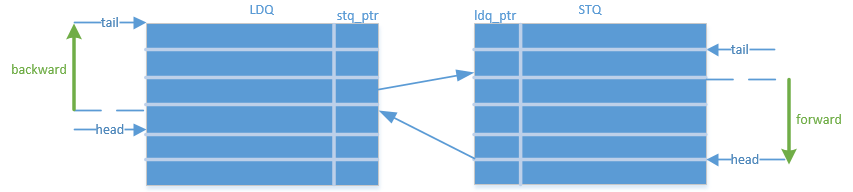
\includegraphics[width=\linewidth]{fwdbwd}
	\caption{forward \& backward示意图}
\end{figure}

为了确定forward和backward的起点,在原来的队列中各要加入指针域,在LDQ中是索引STQ的指针stq\_ptr,在STQ中是索引LDQ的指针ldq\_ptr。
\subsection{特权态指令执行的初步方案}
前面提到的后端各个数据结构大多都是针对用户态指令的,而特权态指令相对稀少而且特殊,目前还没有来得及针对risc-v好好分析一下特权态指令的依赖关系来进行优化,初步的方案是特权指令一律不会进入发射队列乱序化,而且一定要等到ROB为空时才能够直接发射执行。
\subsection{后端状态回溯机制}
状态的回溯在前面中间层的CPU状态控制单元已经有所提及,除了CPU状态控制单元负责CPU状态的回溯以外,对于后端其他数据结构的状态回溯因为有一个很好的抽象也就显得非常的简单直观。这是因为后端和中间层都是由队列构成的,或者是移位队列或者是循环队列。对于移位队列,如果是例外中断或者访存回滚,计数器置为0即可;如果是跳转指令取缔,将计数器置为id号小于该跳转指令的指令个数。对于循环队列,同理操纵head和tail指针即可。
\section{总结}
前端的章节中已经提到取指器的时序非常好,所有从后端传递的反馈信号都是锁一拍才会对取指器产生作用。而BTB也对其数据结构做了相应的物理的优化。前端是3级的流水,指令在第3级产生,被送到连接前后端的中间层,中间层先经过重命名把逻辑寄存器地址转化为物理寄存器地址,紧接着去索引物理寄存器堆读取数据出来直接送到锁存器,或者其实物理寄存器可以做成一个同步ram。CPU的最长路径极有可能会是这一条,目测估计要经过34级们左右。与这条路径并行的是物理资源的分配以及精确发射。如果发射队列为空就直接可以进入执行级执行,否则先进入发射队列轮循侦结果总线和旁路总线的信号。结果总线顾名思义就是结果已经得到的写回信息,而旁路总线指的是当前正要被发射,正在重命名读寄存器送到exe级执行的信号,换言之是预言下一拍就会得到结果的前递信号。由于commit总线的宽度是4,regfile的的写端口是4个,所以两类前递总线各有4组,总共8组。前递逻辑是时序也是比较紧张的,目测和中间层逻辑门级数要少一两级,但是相差不大。执行级依据内部微码对操作数进行运算,当然被送到exe级存在操作数还没有准备好的情况,将其压入执行队列。但是执行队列限定每一次只允许一条指令入队。处于平衡队列的考虑,如果同时出现两个发射队列的头部都没有准备好操作数,优先选择指令条数多的队列的头部指令入队。对于跳转指令和访存指令这种特定类别的指令执行控制,参考。%TODO

\chapter{分析与讨论}\label{chap:analysis}


	
\chapter{结论与展望}\label{chap:future}
%icache目前还是直接映射的。
%被诟病的微结构
%截至中期,工程实现依旧采用的是直接映射的存储结构,后期会将其调整为4路组相连结构。这里有两个目的。其一,risc-v对于页表的规定固定为4KB,为了做到cpu的tlb虚实转化和访问cache的并行,所以cache core的每一路的容量都至多是4KB,也就是说用虚实地址共享的地址(不用tlb cam来进行虚实转换)来索引cache core。但是4KB的容量显然不够的,但是每一路至多4KB,当然可以用硬件来解决顶着色对每一路的cache core进行扩容,但是这就很复杂了。所以另一种思路就是增加路数,比如四路;其二,四路比一路cache的替换率要低,这不光是容量的问题,四路的每路4KB的cache在一般情况下要比容量相同的16KB的单路cache的替换率都低。

%所以对于cache core最终的组织形式目前的想法是4路组相连,每一路4KB,采用LRU或者随机替换或者一种兼而有之的方法。不会参考alpha21464一样做路预测,一是为了降低复杂度,二是因为估计在自己的设计中延迟时序允许。
%基于CAM的重命名表
%更侧重微结构的设计
	通过章节\ref{chap:analysis}的分析,相比于单发射五级静态流水线再到双发射五级静态流水线,双发射乱序处理器在执行程序的效率上有了比较明显的提升。但是另一方面,也可以看出双发射乱序处理器对于转移猜测的预测率是非常敏感的,一些测试程序如coremark和meidian由于目前实现的转移预测正确率不到80\%,而导致在没有访存延迟的情况下,反而比双发射五级静态流水IPC要差。所以当务之急是通过牺牲面积的方式引入效果更好的转移预测方式,提高转移预测率从而提高双发射乱序执行程序的效率。这也是前端的首要改进工作。对于中间层,在最近的一段时间内,通过仔细的思考,发现基于CAM的重命名表会比基于RAM的重命名表面积更小,时序更好,而且逻辑同样的简单。对于后端,首要的任务是加入非阻塞式的dcache,包括对后端时序更为细致的打磨。
	
	所以对于眼前的展望就是将这个超标量宽度为2的双发射乱序处理器的效率继续提升。对于稍远的计划,还是要把整个系统做大做完整,比如做成64位架构的,然后加入浮点的逻辑,使之能够成为像BOOM一样具有实用价值的处理器核。而且光从流水线的划分粗略的分析,在同为前端超标量宽度为2的设置下,后端设计的调度策略和机制是比BOOMv2更好,时序上粗略估计也不必BOOM差。所以在做出完整系统的同时,性能上的目标是要超过BOOMv2,基本上要做到ARM Cortex A57的水平。更长远的展望是,因为国内的大方向还是以MIPS体系结构为主,所以肯定会将目前基于RISC-V的设计改版成MIPS的版本,然后通过不懈的努力,使自己的设计像BOOM一样能够有机会流片,在实际的应用中得到检验。
	
	
	
%\chapter{\LaTeX{}使用说明}\label{chap:guide}

为方便使用及更好地展示\LaTeX{}排版的优秀特性,ucasthesis的框架和文件体系进行了细致地处理,尽可能地对各个功能和板块进行了模块化和封装,对于初学者来说,众多的文件目录也许一开始让人觉得有些无所适从,但阅读完下面的使用说明后,会发现原来使用思路是简单而清晰的,而且,当对\LaTeX{}有一定的认识和了解后,会发现其相对Word类排版系统极具吸引力的优秀特性。所以,如果是初学者,请不要退缩,请稍加尝试和坚持,以领略到\LaTeX{}的非凡魅力,并可以通过阅读相关资料如\LaTeX{} Wikibook\citep{wikibook2014latex}来完善自己的使用知识。

\section{先试试效果}

\begin{enumerate}
    \item 安装软件:根据所用操作系统和章节~\ref{sec:system}中的信息安装\LaTeX{}编译环境。
    \item 获取模板:下载 \href{https://github.com/mohuangrui/ucasthesis}{ucasthesis} 模板并解压。ucasthesis模板不仅提供了相应的类文件,同时也提供了包括参考文献等在内的完成学位论文的一切要素,所以,下载时,推荐下载整个ucasthesis文件夹,而不是单独的文档类。
    \item 编译模板:
        \begin{enumerate}
            \item Windows:双击运行artratex.bat脚本。
            \item Linux或MacOS: {\scriptsize \verb|terminal| -> \verb|chmod +x ./artratex.sh| -> \verb|./artratex.sh xa|}
            \item 任意系统:都可使用\LaTeX{}编辑器打开Thesis.tex文件并选择xelatex编译引擎进行编译。
        \end{enumerate}
    \item 错误处理:若编译中遇到了问题,请先查看“常见问题”(章节~\ref{sec:qa})。
\end{enumerate}

编译完成即可获得本PDF说明文档。而这也完成了学习使用ucasthesis撰写论文的一半进程。什么?这就学成一半了,这么简单???,是的,就这么简单!

\section{文档目录简介}

\subsection{Thesis.tex}

Thesis.tex为主文档,其设计和规划了论文的整体框架,通过对其的阅读可以了解整个论文框架的搭建。

\subsection{编译脚本}

\begin{itemize}
    \item Windows:双击Dos脚本artratex.bat可得全编译后的PDF文档,其存在是为了帮助不了解\LaTeX{}编译过程的初学者跨过编译这第一道坎,请勿通过邮件传播和接收此脚本,以防范Dos脚本的潜在风险。
    \item Linux或MacOS:在terminal中运行
        \begin{itemize}
            \item \verb|./artratex.sh xa|:获得全编译后的PDF文档
            \item \verb|./artratex.sh x|:快速编译模式
        \end{itemize}
    \item 全编译指运行 \verb|xelatex+bibtex+xelatex+xelatex| 以正确生成所有的引用链接,如目录,参考文献及引用等。在写作过程中若无添加新的引用,则可用快速编译,即只运行一遍\LaTeX{}编译引擎以减少编译时间。
\end{itemize}

\subsection{Tmp文件夹}

运行编译脚本后,编译所生成的文档皆存于Tmp文件夹内,包括编译得到的PDF文档,其存在是为了保持工作空间的整洁,因为好的心情是很重要的。

\subsection{Style文件夹}

包含ucasthesis文档类的定义文件和配置文件,通过对它们的修改可以实现特定的模版设定。若需更新模板,一般只需用新的样式文件替换旧的即可。

\begin{enumerate}
    \item ucasthesis.cls:文档类定义文件,论文的最核心的格式即通过它来定义的。
    \item ucasthesis.cfg:文档类配置文件,设定如目录显示为“目~录”而非“目录”。
    \item artratex.sty: 常用宏包及文档设定,如参考文献样式、文献引用样式、页眉页脚设定等。这些功能具有开关选项,常只需在Thesis.tex中的如下命令中进行启用即可,一般无需修改artratex.sty本身。
        
        \path{\usepackage[options]{artratex}} 
    \item artracom.sty:自定义命令以及添加宏包的推荐放置位置。
\end{enumerate}

\subsection{Tex文件夹}

文件夹内为论文的所有实体内容,正常情况下,这也是\textbf{使用ucasthesis撰写学文论文时,主要关注和修改的一个位置,注:所有文件都必须采用UTF-8编码,否则编译后将出现乱码文本},详细分类介绍如下:

\begin{itemize}
    \item Frontpage.tex:为论文中英文封面及中英文摘要。\textbf{论文封面会根据英文学位名称如Bachelor,Master,或是Doctor自动切换为相应的格式}。
    \item Mainmatter.tex:索引需要出现的Chapter。开始写论文时,可以只索引当前章节,以快速编译查看,当论文完成后,再对所有章节进行索引即可。
    \item Chap{\_}xxx.tex:为论文主体的各个章节,可根据需要添加和撰写。
    \item Appendix.tex:为附录内容
    \item Backmatter.tex:为发表文章信息和致谢部分等。
\end{itemize}

\subsection{Img文件夹}

用于放置论文中所需要的图类文件,支持格式有:.jpg, .png, .pdf。其中,\verb|ucas_logo.pdf|为国科大校徽。不建议为各章节图片建子目录,即使图片众多,若命名规则合理,图片查询亦是十分方便。

\subsection{Biblio文件夹}

\begin{enumerate}
    \item ref.bib:参考文献信息库。
    \item gbt7714-xxx.bst:符合国标的文献样式定义文件。由 \href{https://github.com/zepinglee/gbt7714-bibtex-style}{zepinglee}  开发,并满足最新国标要求。与文献样式有关的问题,请查阅开发者所提供的文档,并建议适当追踪其更新。
\end{enumerate}

\section{数学公式、图表、参考文献等功能}

\subsection{数学公式}

比如Navier-Stokes方程:
\begin{equation} \label{eq:ns}
    \begin{cases}
        \frac{\partial \rho}{\partial t} + \nabla\cdot(\rho\Vector{V}) = 0 \ \mathrm{times\ font\ test}\\
        \frac{\partial (\rho\Vector{V})}{\partial t} + \nabla\cdot(\rho\Vector{V}\Vector{V}) = \nabla\cdot\Tensor{\sigma} \ \text{times font test}\\
        \frac{\partial (\rho E)}{\partial t} + \nabla\cdot(\rho E\Vector{V}) = \nabla\cdot(k\nabla T) + \nabla\cdot(\Tensor{\sigma}\cdot\Vector{V})
    \end{cases}
\end{equation}
\begin{equation}
    \frac{\partial }{\partial t}\int\limits_{\Omega} u \, \mathrm{d}\Omega + \int\limits_{S} \unitVector{n}\cdot(u\Vector{V}) \, \mathrm{d}S = \dot{\phi}
\end{equation}

数学公式常用命令请见 \href{https://en.wikibooks.org/wiki/LaTeX/Mathematics}{WiKibook Mathematics}。artracom.sty中对一些常用数据类型如矢量矩阵等进行了封装,这样的好处是如有一天需要修改矢量的显示形式,只需单独修改artracom.sty中的矢量定义即可实现全文档的修改。

\subsection{表格}

请见表~\ref{tab:sample}。制表的更多范例,请见 \href{https://en.wikibooks.org/wiki/LaTeX/Tables}{WiKibook Tables}。
\begin{table}[!htbp]
    \bicaption{这是一个样表。}{This is a sample table.}
    \label{tab:sample}
    \centering
    \footnotesize% fontsize
    \setlength{\tabcolsep}{4pt}% column separation
    \renewcommand{\arraystretch}{1.2}%row space 
    \begin{tabular}{lcccccccc}
        \hline
        Row number & \multicolumn{8}{c}{This is a multicolumn} \\
        %\cline{2-9}% partial hline from column i to column j
        \hline
        Row 1 & $1$ & $2$ & $4$ & $5$ & $6$ & $7$ & $8$\\
        Row 2 & $1$ & $2$ & $4$ & $5$ & $6$ & $7$ & $8$\\
        Row 3 & $1$ & $2$ & $4$ & $5$ & $6$ & $7$ & $8$\\
        Row 4 & $1$ & $2$ & $4$ & $5$ & $6$ & $7$ & $8$\\
        \hline
    \end{tabular}
\end{table}

\subsection{图片插入}

论文中图片的插入通常分为单图和多图,下面分别加以介绍:

单图插入:假设插入名为\verb|tc_q_criteria|(后缀可以为.jpg、.png、.pdf,下同)的图片,其效果如图\ref{fig:tc_q_criteria}。
\begin{figure}[!htbp]
    \centering
    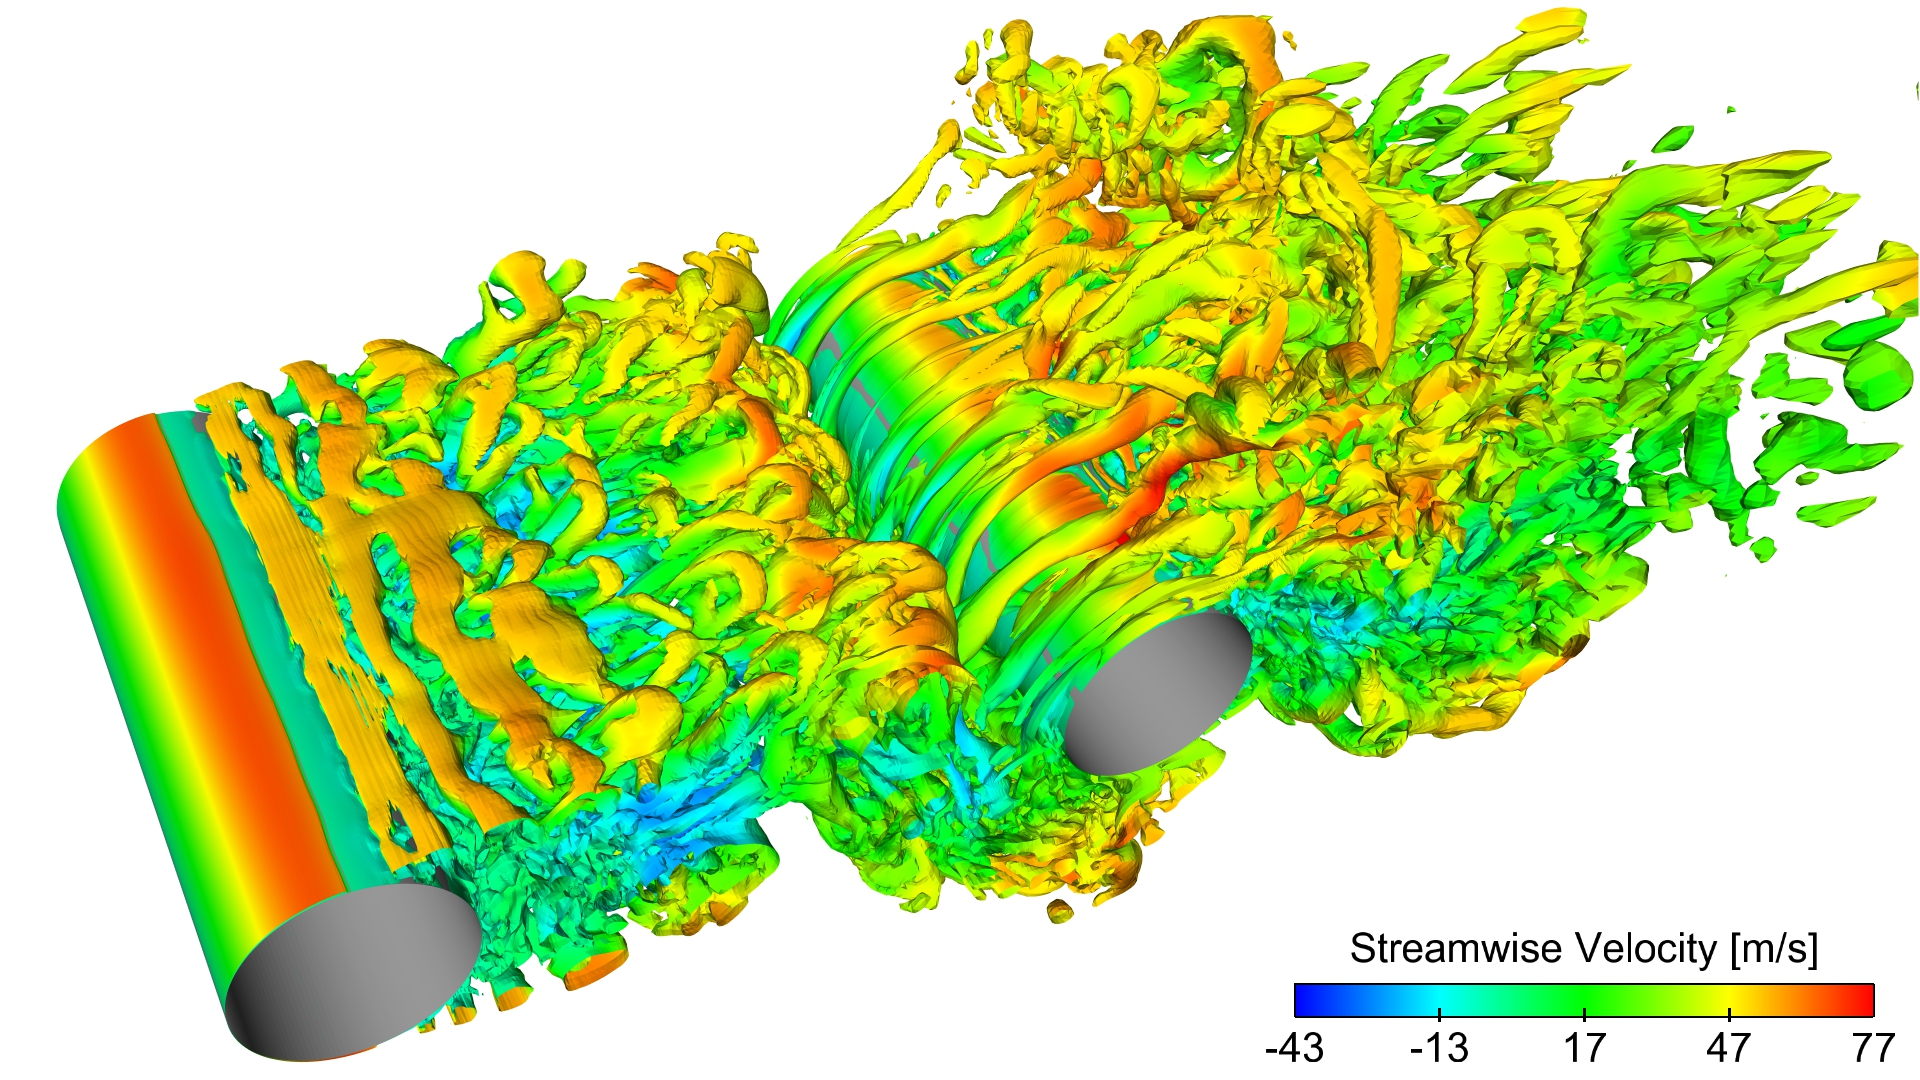
\includegraphics[width=0.40\textwidth]{tc_q_criteria}
    \bicaption{Q判据等值面图,同时测试一下一个很长的标题,比如这真的是一个很长很长很长很长很长很长很长很长的标题。}{Isocontour of Q criteria, at the same time, this is to test a long title, for instance, this is a really very long very long very long very long very long title.}
    \label{fig:tc_q_criteria}
\end{figure}

如果插图的空白区域过大,以图片\verb|shock_cyn|为例,自动裁剪如图\ref{fig:shock_cyn}。
\begin{figure}[!htbp]
    \centering
    %trim option's parameter order: left bottom right top
    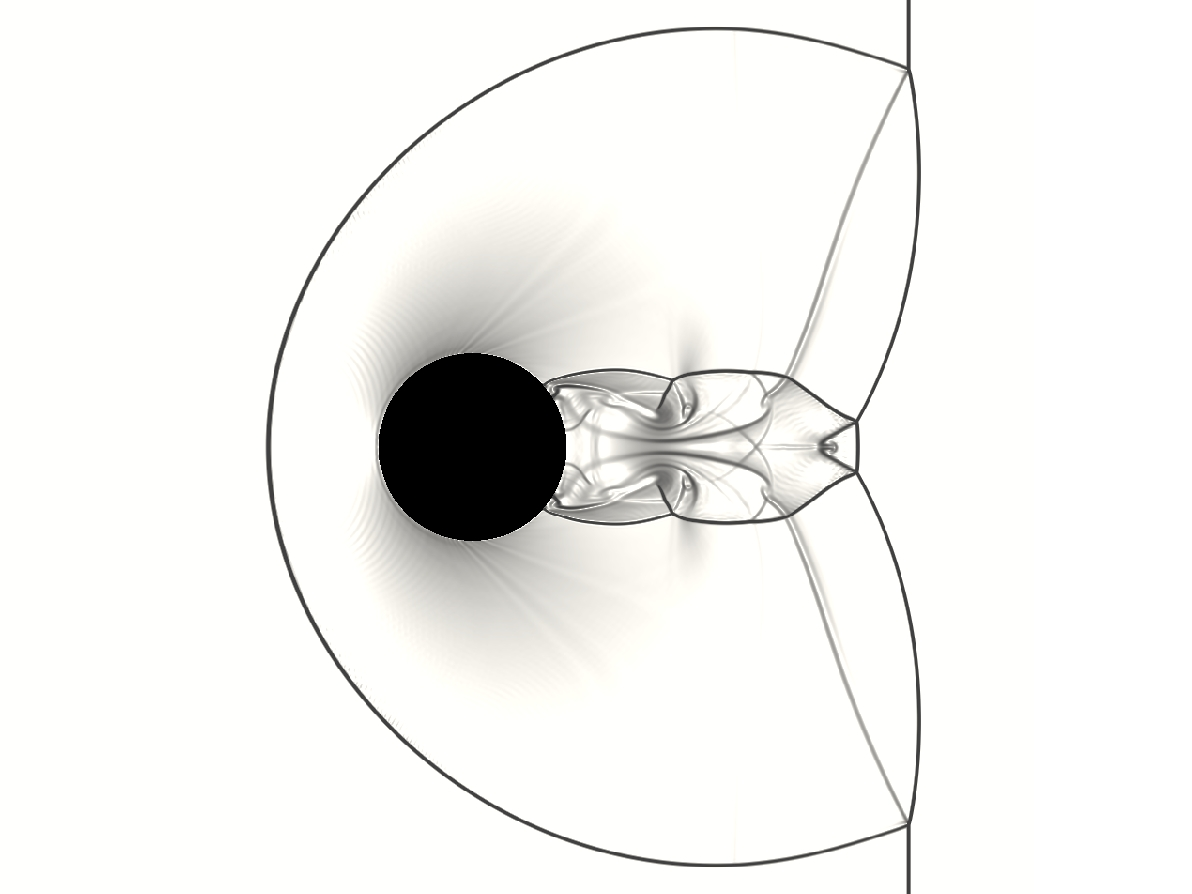
\includegraphics[trim = 30mm 0mm 30mm 0mm, clip, width=0.40\textwidth]{shock_cyn}
    \bicaption{激波圆柱作用。}{Shock-cylinder interaction.}
    \label{fig:shock_cyn}
\end{figure}

多图的插入如图\ref{fig:oaspl},多图不应在子图中给文本子标题,只要给序号,并在主标题中进行引用说明。
\begin{figure}[!htbp]
    \centering
    \begin{subfigure}[b]{0.35\textwidth}
      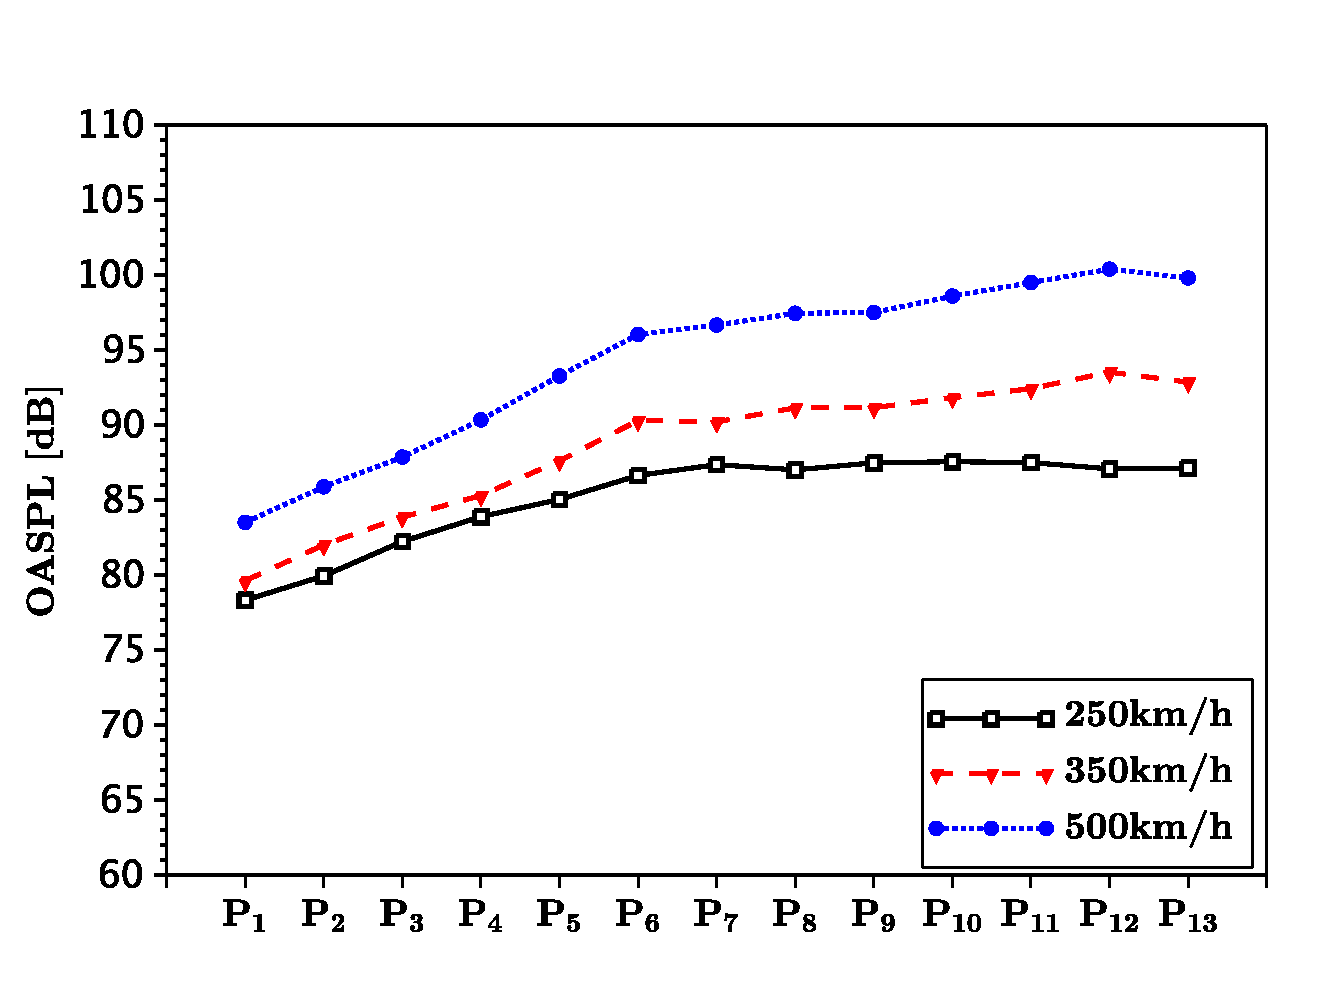
\includegraphics[width=\textwidth]{oaspl_a}
      \caption{}
      \label{fig:oaspl_a}
    \end{subfigure}%
    ~%add desired spacing
    \begin{subfigure}[b]{0.35\textwidth}
      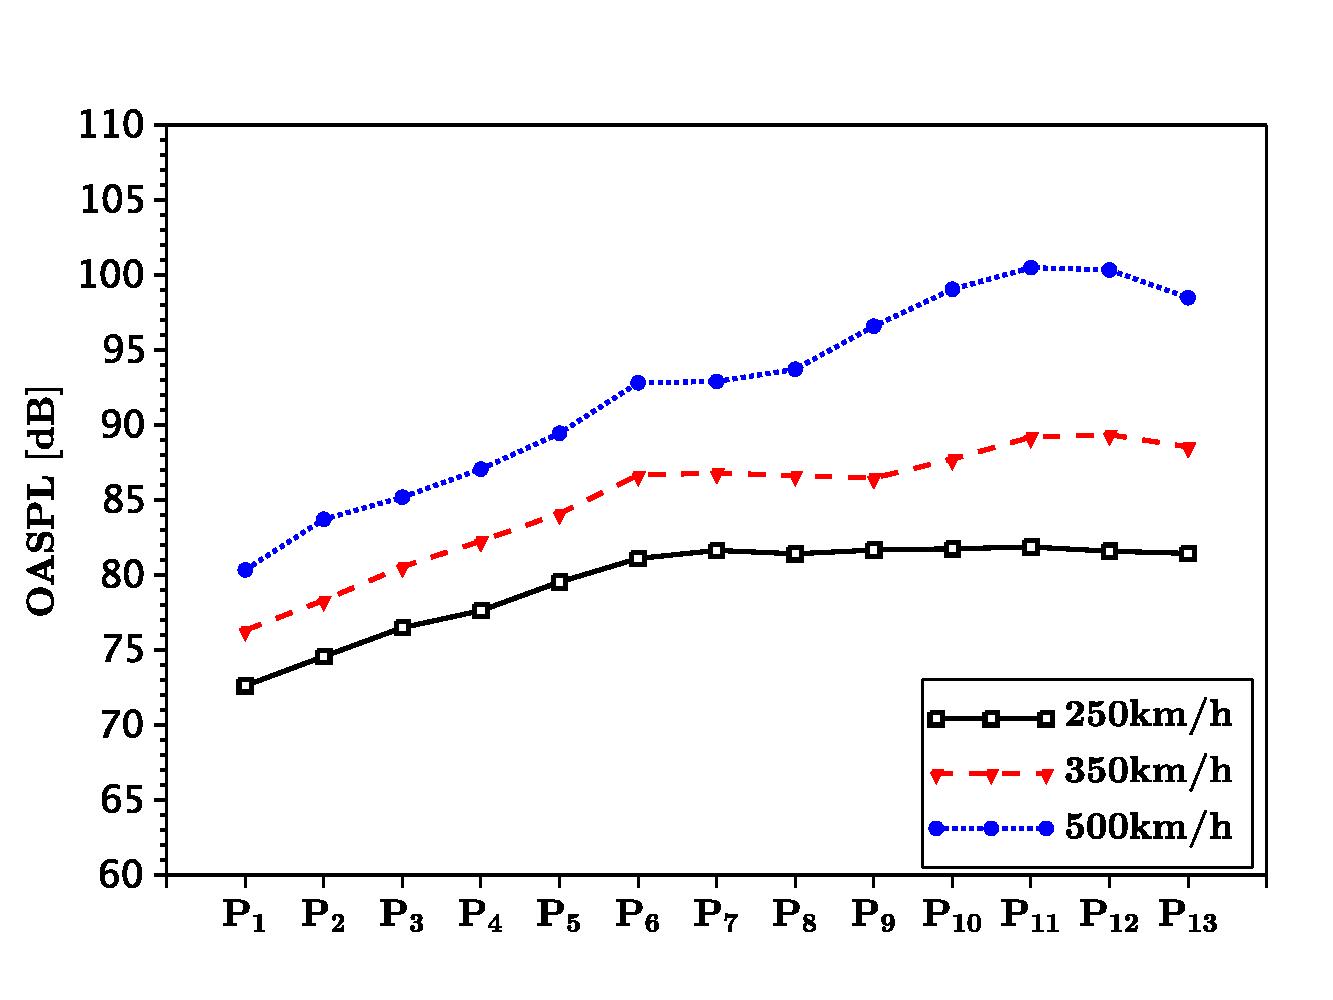
\includegraphics[width=\textwidth]{oaspl_b}
      \caption{}
      \label{fig:oaspl_b}
    \end{subfigure}
    \begin{subfigure}[b]{0.35\textwidth}
      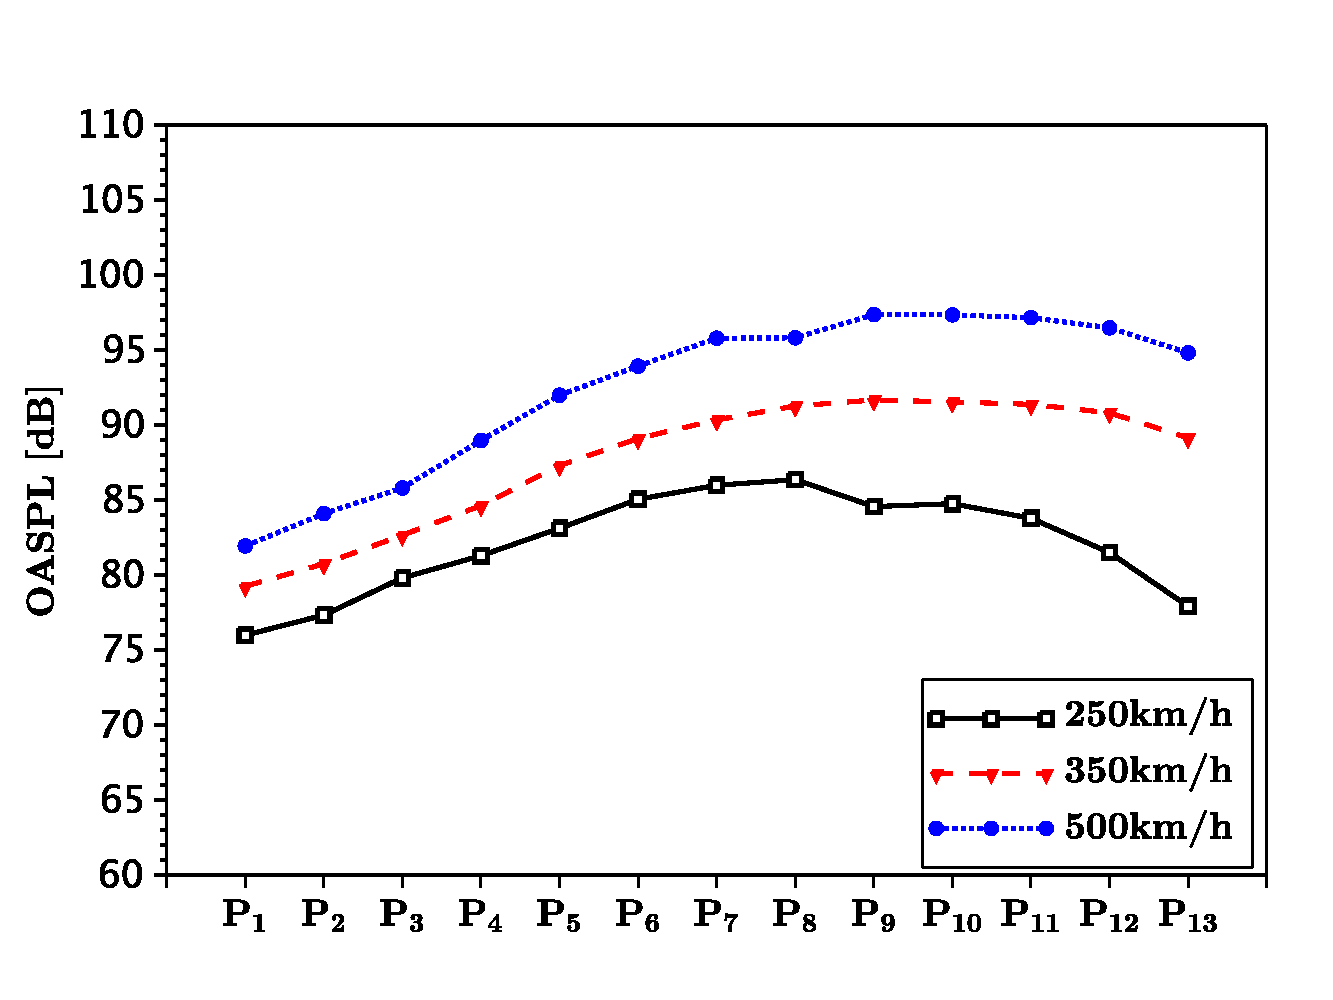
\includegraphics[width=\textwidth]{oaspl_c}
      \caption{}
      \label{fig:oaspl_c}
    \end{subfigure}%
    ~%add desired spacing
    \begin{subfigure}[b]{0.35\textwidth}
      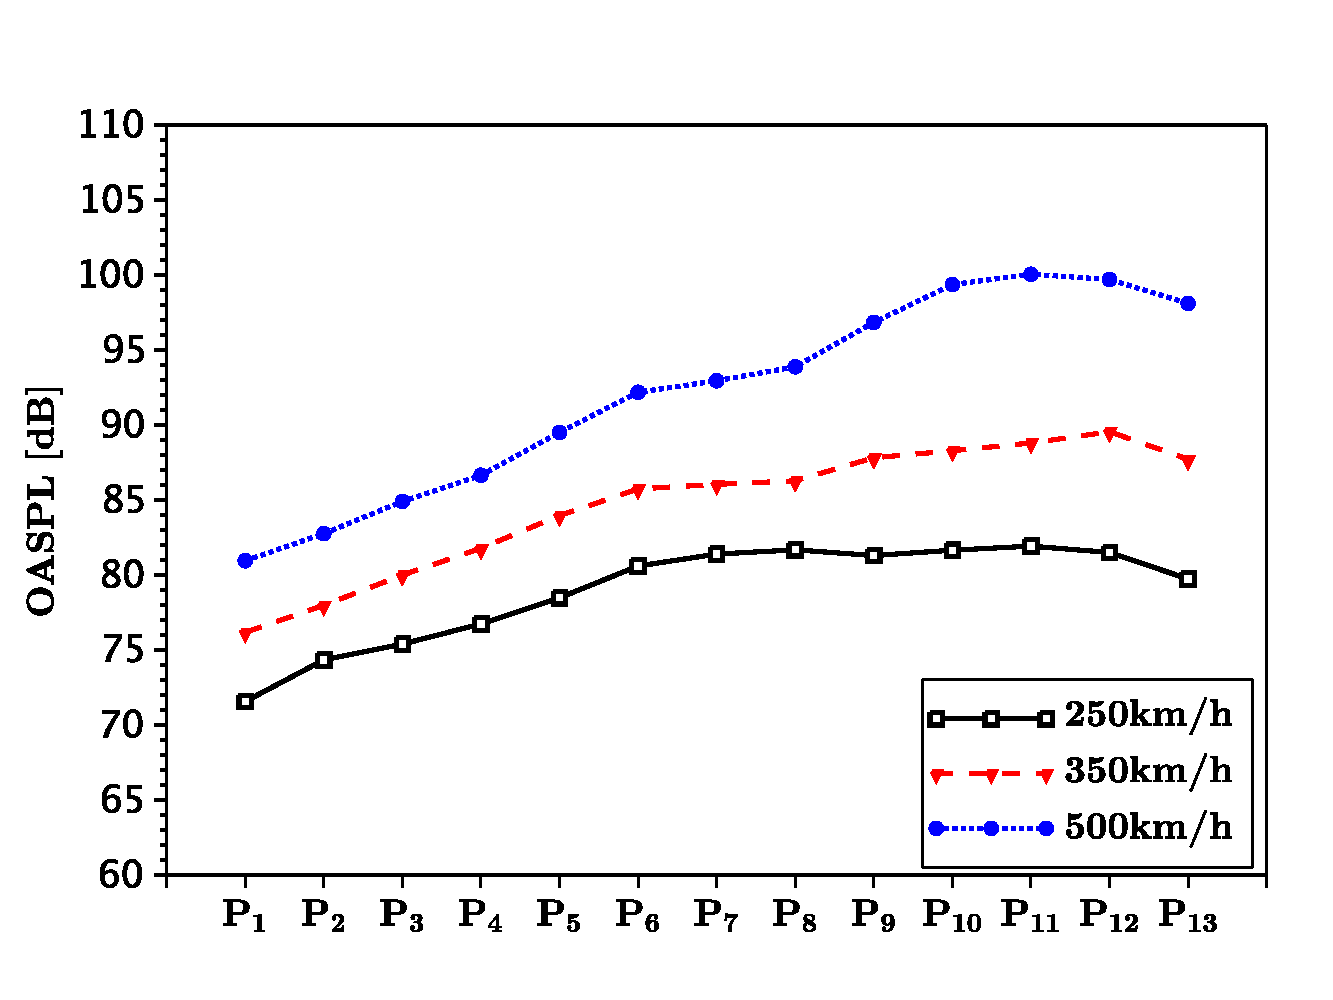
\includegraphics[width=\textwidth]{oaspl_d}
      \caption{}
      \label{fig:oaspl_d}
    \end{subfigure}
    \bicaption{总声压级。(a) 这是子图说明信息,(b) 这是子图说明信息,(c) 这是子图说明信息,(d) 这是子图说明信息。}{OASPL.(a) This is the explanation of subfig, (b) This is the explanation of subfig, (c) This is the explanation of subfig, (d) This is the explanation of subfig.}
    \label{fig:oaspl}
\end{figure}

\subsection{算法}

如见算法~\ref{alg:euclid},详细使用方法请参见文档 \href{https://ctan.org/pkg/algorithmicx?lang=en}{algorithmicx}。

\begin{algorithm}[!htbp]
    \small
    \caption{Euclid's algorithm}\label{alg:euclid}
    \begin{algorithmic}[1]
        \Procedure{Euclid}{$a,b$}\Comment{The g.c.d. of a and b}
        \State $r\gets a\bmod b$
        \While{$r\not=0$}\Comment{We have the answer if r is 0}
        \State $a\gets b$
        \State $b\gets r$
        \State $r\gets a\bmod b$
        \EndWhile\label{euclidendwhile}
        \State \textbf{return} $b$\Comment{The gcd is b}
        \EndProcedure
    \end{algorithmic}
\end{algorithm}

\subsection{参考文献引用}

参考文献引用过程以实例进行介绍,假设需要引用名为"Document Preparation System"的文献,步骤如下:

1)使用Google Scholar搜索Document Preparation System,在目标条目下点击Cite,展开后选择Import into BibTeX打开此文章的BibTeX索引信息,将它们copy添加到ref.bib文件中(此文件位于Biblio文件夹下)。

2)索引第一行 \verb|@article{lamport1986document,|中 \verb|lamport1986document| 即为此文献的label (\textbf{中文文献也必须使用英文label},一般遵照:姓氏拼音+年份+标题第一字拼音的格式),想要在论文中索引此文献,有两种索引类型:

文本类型:\verb|\citet{lamport1986document}|。正如此处所示 \citet{lamport1986document}; 

括号类型:\verb|\citep{lamport1986document}|。正如此处所示 \citep{lamport1986document}。

\textbf{多文献索引用英文逗号隔开}:

\verb|\citep{lamport1986document, chu2004tushu, chen2005zhulu}|。正如此处所示 \citep{lamport1986document, chu2004tushu, chen2005zhulu}

更多例子如:

\citet{walls2013drought}根据...的研究,首次提出...。其中关于...\citep{walls2013drought},是当前中国...得到迅速发展的研究领域\citep{chen1980zhongguo}。引用同一著者在同一年份出版的多篇文献时,在出版年份之后用
英文小写字母区别,如:\citep{yuan2012lana, yuan2012lanb, yuan2012lanc}。同一处引用多篇文献时,按出版年份由近及远依次标注,中间用
分号分开。例如\citep{chen1980zhongguo, stamerjohanns2009mathml, hls2012jinji, niu2013zonghe}。

使用著者-出版年制(authoryear)式参考文献样式时,中文文献必须在BibTeX索引信息的 \textbf{key} 域(请参考ref.bib文件)填写作者姓名的拼音,才能使得文献列表按照拼音排序。参考文献表中的条目(不排序号),先按语种分类排列,语种顺 序是:中文、日文、英文、俄文、其他文种。然后,中文按汉语拼音字母顺序排列,日文按第一著者的姓氏笔画排序,西文和 俄文按第一著者姓氏首字母顺序排列。如中\citep{niu2013zonghe}、日\citep{Bohan1928}、英\citep{stamerjohanns2009mathml}、俄\citep{Dubrovin1906}。

如此,即完成了文献的索引,请查看下本文档的参考文献一章,看看是不是就是这么简单呢?是的,就是这么简单!

不同文献样式和引用样式,如著者-出版年制(authoryear)、顺序编码制(numbers)、上标顺序编码制(super)可在Thesis.tex中对artratex.sty调用实现,如:
\begin{itemize}
    \footnotesize
    \item \verb+\usepackage[numbers]{artratex}+ $\%$ 文本: Jones [1]; 括号: [1]
    \item \verb+\usepackage[super]{artratex}+ $\%$ 文本: Jones 上标[1]; 括号: 上标[1]
    \item \verb+\usepackage[authoryear]{artratex}+ $\%$ 文本: Jones (1995); 括号: (Jones, 1995)
    \item \verb+\usepackage[alpha]{artratex}+ $\%$ 文本: 不可用; 括号: [Jon95]
\end{itemize}

当前文档的默认参考文献样式为\textbf{authoryear}。若在上标(\textbf{super})模式下,希望在特定位置将上标改为嵌入式标,可使用

文本类型:\verb|\citetns{lamport1986document,chen2005zhulu}|。

正如此处所示\citetns{lamport1986document,chen2005zhulu}

括号类型:\verb|\citepns{lamport1986document,chen2005zhulu}|。

正如此处所示\citepns{lamport1986document,chen2005zhulu}

参考文献索引更为详细的信息,请见 \href{https://github.com/zepinglee/gbt7714-bibtex-style}{zepinglee} 和 \href{https://en.wikibooks.org/wiki/LaTeX/Bibliography_Management}{WiKibook Bibliography}。

\nocite{*}

\section{常见使用问题}\label{sec:qa}

\begin{enumerate}
    \item 模板每次发布前,都已在Windows,Linux,MacOS系统上测试通过。下载模板后,若编译出现错误,则请见 \href{https://github.com/mohuangrui/ucasthesis/wiki}{ucasthesis和\LaTeX{}知识小站} 的 \href{https://github.com/mohuangrui/ucasthesis/wiki/%E7%BC%96%E8%AF%91%E6%8C%87%E5%8D%97}{编译指南}。

    \item 模板文档的编码为UTF-8编码。所有文件都必须采用UTF-8编码,否则编译后生成的文档将出现乱码文本。若出现文本编辑器无法打开文档或打开文档乱码的问题,请检查编辑器对UTF-8编码的支持。如果使用WinEdt作为文本编辑器(\textbf{不推荐使用}),应在其Options -> Preferences -> wrapping选项卡下将两种Wrapping Modes中的内容:
        
        TeX;HTML;ANSI;ASCII|DTX...
        
        修改为:TeX;\textbf{UTF-8|ACP;}HTML;ANSI;ASCII|DTX...
        
        同时,取消Options -> Preferences -> Unicode中的Enable ANSI Format。

    \item 推荐选择xelatex或lualatex编译引擎编译中文文档。编译脚本的默认设定为xelatex编译引擎。你也可以选择不使用脚本编译,如直接使用 \LaTeX{}文本编辑器编译。注:\LaTeX{}文本编辑器编译的默认设定为pdflatex编译引擎,若选择xelatex或lualatex编译引擎,请进入下拉菜单选择。为正确生成引用链接,需要进行全编译。

    \item Texmaker使用简介
        \begin{enumerate}
            \footnotesize
            \item 使用 Texmaker “打开 (Open)” Thesis.tex。
            \item 菜单 “选项 (Options)” -> “设置当前文档为主文档 (Define as Master Document)”
            \item 菜单 “自定义 (User)” -> “自定义命令 (User Commands)” -> “编辑自定义命令 (Edit User Commands)” -> 左侧选择 “command 1”,右侧 “菜单项 (Menu Item)” 填入 Auto Build -> 点击下方“向导 (Wizard)” -> “添加 (Add)”: xelatex + bibtex + xelatex + xelatex + pdf viewer -> 点击“完成 (OK)”
            \item 使用 Auto Build 编译带有未生成引用链接的源文件,可以仅使用 xelatex 编译带有已经正确生成引用链接的源文件。
            \item 编译完成,“查看(View)” PDF,在PDF中 “ctrl+click” 可链接到相对应的源文件。
        \end{enumerate}
    
    \item 模版的设计可能地考虑了适应性。致谢等所有条目都是通过最为通用的

        \verb+\chapter{item name}+  and \verb+\section*{item name}+

        来显式实现的 (请观察Backmatter.tex),从而可以随意添加,放置,和修改,如同一般章节。对于图表目录名称则可在ucasthesis.cfg中进行修改。

    \item 设置文档样式: 在artratex.sty中搜索关键字定位相应命令,然后修改
        \begin{enumerate}
            \item 正文行距:启用和设置 \verb|\linespread{1.5}|,默认1.5倍行距。
            \item 参考文献行距:修改 \verb|\setlength{\bibsep}{0.0ex}|
            \item 目录显示级数:修改 \verb|\setcounter{tocdepth}{2}|
            \item 文档超链接的颜色及其显示:修改 \verb|\hypersetup|
        \end{enumerate}

    \item 文档内字体切换方法:
        \begin{itemize}
            \item 宋体:国科大论文模板ucasthesis 或 \textrm{国科大论文模板ucasthesis}
            \item 粗宋体:{\bfseries 国科大论文模板ucasthesis} 或 \textbf{国科大论文模板ucasthesis}
            \item 黑体:{\sffamily 国科大论文模板ucasthesis} 或 \textsf{国科大论文模板ucasthesis}
            \item 粗黑体:{\bfseries\sffamily 国科大论文模板ucasthesis} 或 \textsf{\bfseries 国科大论文模板ucasthesis}
            \item 仿宋:{\ttfamily 国科大论文模板ucasthesis} 或 \texttt{国科大论文模板ucasthesis}
            \item 粗仿宋:{\bfseries\ttfamily 国科大论文模板ucasthesis} 或 \texttt{\bfseries 国科大论文模板ucasthesis}
            \item 楷体:{\itshape 国科大论文模板ucasthesis} 或 \textit{国科大论文模板ucasthesis}
            \item 粗楷体:{\bfseries\itshape 国科大论文模板ucasthesis} 或 \textit{\bfseries 国科大论文模板ucasthesis}
        \end{itemize}

    \item 封面下划线上的文本不居中下划线,这是因为下划线前面还有字头,导致文本只能在页面居中和在下划线上居中二选一。当前封面采取页面居中。如需要调整文本在下划线上的位置,可用 \verb|\hspace{+/- n.0em}| 命令来插入或删除 n 个空格,进行手动调整,比如

        \verb|\advisor{\hspace{+3.0em} xxx~研究员~xxx单位}|
                
    有时下划线看上去粗细不一致,这是显示的问题,打印正常。
\end{enumerate}



%---------------------------------------------------------------------------%
% main content
%-
%-> Appendix
%-
\cleardoublepage%
\appendix% initialize the environment
%\chapter{中国科学院大学学位论文撰写要求}

学位论文是研究生科研工作成果的集中体现,是评判学位申请者学术水平、授予其学位的主要依据,是科研领域重要的文献资料。根据《科学技术报告、学位论文和学术论文的编写格式》(GB/T 7713-1987)、《学位论文编写规则》(GB/T 7713.1-2006)和《文后参考文献著录规则》(GB7714—87)等国家有关标准,结合中国科学院大学(以下简称“国科大”)的实际情况,特制订本规定。

\section{论文无附录者无需附录部分}

\section{测试公式编号} \label{sec:testmath}

\begin{equation} \label{eq:appedns}
    \begin{cases}
        \frac{\partial \rho}{\partial t} + \nabla\cdot(\rho\Vector{V}) = 0 \ \mathrm{times\ font\ test}\\
        \frac{\partial (\rho\Vector{V})}{\partial t} + \nabla\cdot(\rho\Vector{V}\Vector{V}) = \nabla\cdot\Tensor{\sigma} \ \text{times font test}\\
        \frac{\partial (\rho E)}{\partial t} + \nabla\cdot(\rho E\Vector{V}) = \nabla\cdot(k\nabla T) + \nabla\cdot(\Tensor{\sigma}\cdot\Vector{V})
    \end{cases}
\end{equation}
\begin{equation}
    \frac{\partial }{\partial t}\int\limits_{\Omega} u \, \mathrm{d}\Omega + \int\limits_{S} \unitVector{n}\cdot(u\Vector{V}) \, \mathrm{d}S = \dot{\phi}
\end{equation}

\section{测试生僻字}

霜蟾盥薇曜灵霜颸妙鬘虚霩淩澌菀枯菡萏泬寥窅冥毰毸濩落霅霅便嬛岧峣瀺灂姽婳愔嫕飒纚棽俪緸冤莩甲摛藻卮言倥侗椒觞期颐夜阑彬蔚倥偬澄廓簪缨陟遐迤逦缥缃鹣鲽憯懔闺闼璀错媕婀噌吰澒洞阛闠覼缕玓瓑逡巡諓諓琭琭瀌瀌踽踽叆叇氤氲瓠犀流眄蹀躞赟嬛茕頔璎珞螓首蘅皋惏悷缱绻昶皴皱颟顸愀然菡萏卑陬纯懿犇麤掱暒 墌墍墎墏墐墒墒墓墔墕墖墘墖墚墛坠墝增墠墡墢墣墤墥墦墧墨墩墪樽墬墭堕墯墰墱墲坟墴墵垯墷墸墹墺墙墼墽垦墿壀壁壂壃壄壅壆坛壈壉壊垱壌壍埙壏壐壑壒压壔壕壖壗垒圹垆壛壜壝垄壠壡坜壣壤壥壦壧壨坝塆圭嫶嫷嫸嫹嫺娴嫼嫽嫾婳妫嬁嬂嬃嬄嬅嬆嬇娆嬉嬊娇嬍嬎嬏嬐嬑嬒嬓嬔嬕嬖嬗嬘嫱嬚嬛嬜嬞嬟嬠嫒嬢嬣嬥嬦嬧嬨嬩嫔嬫嬬奶嬬嬮嬯婴嬱嬲嬳嬴嬵嬶嬷婶嬹嬺嬻嬼嬽嬾嬿孀孁孂娘孄孅孆孇孆孈孉孊娈孋孊孍孎孏嫫婿媚嵭嵮嵯嵰嵱嵲嵳嵴嵵嵶嵷嵸嵹嵺嵻嵼嵽嵾嵿嶀嵝嶂嶃崭嶅嶆岖嶈嶉嶊嶋嶌嶍嶎嶏嶐嶑嶒嶓嵚嶕嶖嶘嶙嶚嶛嶜嶝嶞嶟峤嶡峣嶣嶤嶥嶦峄峃嶩嶪嶫嶬嶭崄嶯嶰嶱嶲嶳岙嶵嶶嶷嵘嶹岭嶻屿岳帋巀巁巂巃巄巅巆巇巈巉巊岿巌巍巎巏巐巑峦巓巅巕岩巗巘巙巚帠帡帢帣帤帨帩帪帬帯帰帱帲帴帵帷帹帺帻帼帽帾帿幁幂帏幄幅幆幇幈幉幊幋幌幍幎幏幐幑幒幓幖幙幚幛幜幝幞帜幠幡幢幤幥幦幧幨幩幪幭幮幯幰幱庍庎庑庖庘庛庝庠庡庢庣庤庥庨庩庪庬庮庯庰庱庲庳庴庵庹庺庻庼庽庿廀厕廃厩廅廆廇廋廌廍庼廏廐廑廒廔廕廖廗廘廙廛廜廞庑廤廥廦廧廨廭廮廯廰痈廲廵廸廹廻廼廽廿弁弅弆弇弉弖弙弚弜弝弞弡弢弣弤弨弩弪弫弬弭弮弰弲弪弴弶弸弻弼弽弿彖彗彘彚彛彜彝彞彟彴彵彶彷彸役彺彻彽彾佛徂徃徆徇徉后徍徎徏径徒従徔徕徖徙徚徛徜徝从徟徕御徢徣徤徥徦徧徨复循徫旁徭微徯徰徱徲徳徴徵徶德徸彻徺忁忂惔愔忇忈忉忔忕忖忚忛応忝忞忟忪挣挦挧挨挩挪挫挬挭挮挰掇授掉掊掋掍掎掐掑排掓掔掕挜掚挂掜掝掞掟掠采探掣掤掦措掫掬掭掮掯掰掱掲掳掴掵掶掸掹掺掻掼掽掾掿拣揁揂揃揅揄揆揇揈揉揊揋揌揍揎揑揓揔揕揖揗揘揙揤揥揦揧揨揫捂揰揱揲揳援揵揶揷揸揻揼揾揿搀搁搂搃搄搅搇搈搉搊搋搌搎搏搐搑搒摓摔摕摖摗摙摚摛掼摝摞摠摡斫斩斮斱斲斳斴斵斶斸旪旫旮旯晒晓晔晕晖晗晘晙晛晜晞晟晠晡晰晣晤晥晦晧晪晫晬晭晰晱晲晳晴晵晷晸晹晻晼晽晾晿暀暁暂暃暄暅暆暇晕晖暊暋暌暍暎暏暐暑暒暓暔暕暖暗旸暙暚暛暜暝暞暟暠暡暣暤暥暦暧暨暩暪暬暭暮暯暰昵暲暳暴暵暶暷暸暹暺暻暼暽暾暿曀曁曂曃晔曅曈曊曋曌曍曎曏曐曑曒曓曔曕曗曘曙曚曛曜曝曞曟旷曡曢曣曤曥曦曧昽曩曪曫晒曭曮曯椗椘椙椚椛検椝椞椟椠椡椢椣椤椥椦椧椨椩椪椫椬椭椮椯椰椱椲椳椴椵椶椷椸椹椺椻椼椽椾椿楀楁楂楃楅楆楇楈楉杨楋楌楍榴榵榶榷榸榹榺榻榼榽榾桤槀槁槂盘槄槅槆槇槈槉槊构槌枪槎槏槐槑槒杠槔槕槖槗滙滛滜滝滞滟滠滢滣滦滧滪滫沪滭滮滰滱渗滳滵滶滹滺浐滼滽漀漃漄漅漈漉溇漋漌漍漎漐漑澙熹漗漘漙沤漛漜漝漞漟漡漤漥漦漧漨漪渍漭漮漯漰漱漳漴溆漶漷漹漺漻漼漽漾浆潀颍潂潃潄潅潆潇潈潉潊潋潌潍潎潏潐潒潓洁潕潖潗潘沩潚潜潝潞潟潠潡潢潣润潥潦潧潨潩潪潫潬潭浔溃潱潲潳潴潵潶滗潸潹潺潻潼潽潾涠澁澄澃澅浇涝澈澉澊澋澌澍澎澏湃澐澑澒澓澔澕澖涧澘澙澚澛澜澝澞澟渑澢澣泽浍澯澰淀澲澳澴澵澶澷澸潇潆瀡瀢瀣瀤瀥潴泷濑瀩瀪瀫瀬瀭瀮瀯弥瀱潋瀳瀴瀵瀶瀷瀸瀹瀺瀻瀼瀽澜瀿灀灁瀺灂沣滠灅灆灇灈灉灊灋灌灍灎灏灐洒灒灓漓灖灗滩灙灚灛灜灏灞灟灠灡灢湾滦灥灦灧灨灪燝燞燠燡燢燣燤燥灿燧燨燩燪燫燮燯燰燱燲燳烩燵燵燸燹燺薰燽焘燿爀爁爂爃爄爅爇爈爉爊爋爌烁爎爏爑爒爓爔爕爖爗爘爙爚烂爜爝爞爟爠爡爢爣爤爥爦爧爨爩猽猾獀犸獂獆獇獈獉獊獋獌獍獏獐獑獒獓獔獕獖獗獘獙獚獛獜獝獞獟獠獡獢獣獤獥獦獧獩狯猃獬獭狝獯狞獱獳獴獶獹獽獾獿猡玁玂玃。
% appendix content
%-
%-> Backmatter: bibliography, glossary, index
%-
\backmatter% initialize the environment
\intotoc{\bibname}% add link to contents table and bookmark
\bibliography{Biblio/ref}% bibliography
% \chapter{作者简历及攻读学位期间发表的学术论文与研究成果}

% \textbf{本科生无需此部分}。

% \section*{作者简历}

% \subsection*{casthesis作者}

% 吴凌云,福建省屏南县人,中国科学院数学与系统科学研究院博士研究生。

% \subsection*{ucasthesis作者}

% 莫晃锐,湖南省湘潭县人,中国科学院力学研究所硕士研究生。

% \section*{已发表(或正式接受)的学术论文:}

% [1] ucasthesis: A LaTeX Thesis Template for the University of Chinese Academy of Sciences, 2014.

% \section*{申请或已获得的专利:}

% (无专利时此项不必列出)

% \section*{参加的研究项目及获奖情况:}

% 可以随意添加新的条目或是结构。

\chapter[致谢]{致\quad 谢}\chaptermark{致\quad 谢}% syntax: \chapter[目录]{标题}\chaptermark{页眉}
\thispagestyle{noheaderstyle}% 如果需要移除当前页的页眉
%\pagestyle{noheaderstyle}% 如果需要移除整章的页眉

%感激casthesis作者吴凌云学长,gbt7714-bibtex-style
%开发者zepinglee,和ctex众多开发者们。若没有他们的辛勤付出和非凡工作,\LaTeX{}菜鸟的我是无法完成此国科大学位论文\LaTeX{}模板ucasthesis的。在\LaTeX{}中的一点一滴的成长源于开源社区的众多优秀资料和教程,在此对所有\LaTeX{}社区的贡献者表示感谢!

%ucasthesis国科大学位论文\LaTeX{}模板的最终成型离不开以霍明虹老师和丁云云老师为代表的国科大学位办公室老师们制定的官方指导文件和众多ucasthesis用户的热心测试和耐心反馈,在此对他们的认真付出表示感谢。特别对国科大的赵永明同学的众多有效反馈意见和建议表示感谢,对国科大本科部的陆晴老师和本科部学位办的丁云云老师的细致审核和建议表示感谢。谢谢大家的共同努力和支持,让ucasthesis为国科大学子使用\LaTeX{}撰写学位论文提供便利和高效这一目标成为可能。
感谢吴瑞阳学长根据自己丰富的工程经验,和我具体而激烈地探讨了处理器初步设计中无论是在电路延迟上,还是在执行效率上存在的问题以及改进的方案。同时,他也给了我很多微结构设计上的有用的意见和电路编写中非常实用的小技巧。

感谢杨灿学姐对于电路时序和龙芯处理器微结构上一些设计的细心答疑,让我对自身的设计有了更好的把控。

\cleardoublepage[plain]% 让文档总是结束于偶数页,可根据需要设定页眉页脚样式,如 [noheaderstyle]

% other information
\end{document}
%---------------------------------------------------------------------------%

